\documentclass[mstat,12pt]{unswthesis}

\usepackage{color}
\usepackage{fancyvrb}
\newcommand{\VerbBar}{|}
\newcommand{\VERB}{\Verb[commandchars=\\\{\}]}
\DefineVerbatimEnvironment{Highlighting}{Verbatim}{commandchars=\\\{\}}
% Add ',fontsize=\small' for more characters per line
\usepackage{framed}
\definecolor{shadecolor}{RGB}{248,248,248}
\newenvironment{Shaded}{\begin{snugshade}}{\end{snugshade}}
\newcommand{\AlertTok}[1]{\textcolor[rgb]{0.94,0.16,0.16}{#1}}
\newcommand{\AnnotationTok}[1]{\textcolor[rgb]{0.56,0.35,0.01}{\textbf{\textit{#1}}}}
\newcommand{\AttributeTok}[1]{\textcolor[rgb]{0.13,0.29,0.53}{#1}}
\newcommand{\BaseNTok}[1]{\textcolor[rgb]{0.00,0.00,0.81}{#1}}
\newcommand{\BuiltInTok}[1]{#1}
\newcommand{\CharTok}[1]{\textcolor[rgb]{0.31,0.60,0.02}{#1}}
\newcommand{\CommentTok}[1]{\textcolor[rgb]{0.56,0.35,0.01}{\textit{#1}}}
\newcommand{\CommentVarTok}[1]{\textcolor[rgb]{0.56,0.35,0.01}{\textbf{\textit{#1}}}}
\newcommand{\ConstantTok}[1]{\textcolor[rgb]{0.56,0.35,0.01}{#1}}
\newcommand{\ControlFlowTok}[1]{\textcolor[rgb]{0.13,0.29,0.53}{\textbf{#1}}}
\newcommand{\DataTypeTok}[1]{\textcolor[rgb]{0.13,0.29,0.53}{#1}}
\newcommand{\DecValTok}[1]{\textcolor[rgb]{0.00,0.00,0.81}{#1}}
\newcommand{\DocumentationTok}[1]{\textcolor[rgb]{0.56,0.35,0.01}{\textbf{\textit{#1}}}}
\newcommand{\ErrorTok}[1]{\textcolor[rgb]{0.64,0.00,0.00}{\textbf{#1}}}
\newcommand{\ExtensionTok}[1]{#1}
\newcommand{\FloatTok}[1]{\textcolor[rgb]{0.00,0.00,0.81}{#1}}
\newcommand{\FunctionTok}[1]{\textcolor[rgb]{0.13,0.29,0.53}{\textbf{#1}}}
\newcommand{\ImportTok}[1]{#1}
\newcommand{\InformationTok}[1]{\textcolor[rgb]{0.56,0.35,0.01}{\textbf{\textit{#1}}}}
\newcommand{\KeywordTok}[1]{\textcolor[rgb]{0.13,0.29,0.53}{\textbf{#1}}}
\newcommand{\NormalTok}[1]{#1}
\newcommand{\OperatorTok}[1]{\textcolor[rgb]{0.81,0.36,0.00}{\textbf{#1}}}
\newcommand{\OtherTok}[1]{\textcolor[rgb]{0.56,0.35,0.01}{#1}}
\newcommand{\PreprocessorTok}[1]{\textcolor[rgb]{0.56,0.35,0.01}{\textit{#1}}}
\newcommand{\RegionMarkerTok}[1]{#1}
\newcommand{\SpecialCharTok}[1]{\textcolor[rgb]{0.81,0.36,0.00}{\textbf{#1}}}
\newcommand{\SpecialStringTok}[1]{\textcolor[rgb]{0.31,0.60,0.02}{#1}}
\newcommand{\StringTok}[1]{\textcolor[rgb]{0.31,0.60,0.02}{#1}}
\newcommand{\VariableTok}[1]{\textcolor[rgb]{0.00,0.00,0.00}{#1}}
\newcommand{\VerbatimStringTok}[1]{\textcolor[rgb]{0.31,0.60,0.02}{#1}}
\newcommand{\WarningTok}[1]{\textcolor[rgb]{0.56,0.35,0.01}{\textbf{\textit{#1}}}}




%%%%%%%%%%%%%%%%%%%%%%%%%%%%%%%%%%%%%%%%%%%%%%%%%%%%%%%%%%%%%%%%%%
% 
% OK...Now we get to some actual input.  The first part sets up
% the title etc that will appear on the front page
%
%%%%%%%%%%%%%%%%%%%%%%%%%%%%%%%%%%%%%%%%%%%%%%%%%%%%%%%%%%%%%%%%%

\title{Hybrid Model Approaches to Improve Short-Term Energy Demand Forecasts in New South Wales, Australia}

\authornameonly{David Valido Ramos (z5516338), Katelyn Kemp (z5459347), Nick Mutton (z5549371), Senarath Seelanatha (z5595581), Shanjay Perinpanathan (z5339723), Waseem Alashqar (z5514810). }

\author{\Authornameonly}

\copyrightfalse
\figurespagefalse
\tablespagefalse

%%%%%%%%%%%%%%%%%%%%%%%%%%%%%%%%%%%%%%%%%%%%%%%%%%%%%%%%%%%%%%%%%
%
%  And now the document begins
%  The \beforepreface and \afterpreface commands puts the
%  contents page etc in
%
%%%%%%%%%%%%%%%%%%%%%%%%%%%%%%%%%%%%%%%%%%%%%%%%%%%%%%%%%%%%%%%%%%


%%%%%%%%%%%%%%%%%%%%%%%%%%%%%%%%%%%%%%%%%%%%%%%%%%%%%%%%%%%%%%%%%%%%%%%
%
%  A small sample UNSW Coursework Masters thesis file.
%  Any questions to Ian Doust i.doust@unsw.edu.au and/or Gery Geenens ggeenens@unsw.edu.au
%
%%%%%%%%%%%%%%%%%%%%%%%%%%%%%%%%%%%%%%%%%%%%%%%%%%%%%%%%%%%%%%%%%%%%%%%
%
%  The first part pulls in a UNSW Thesis class file.  This one is
%  slightly nonstandard and has been set up to do a couple of
%  things automatically
%
 
%%%%%%%%%%%%%%%%%
%% Precisely one of the next four lines should be uncommented.
%% Choose the one which matches your degree, uncomment it, and comment out the other two!
%\documentclass[mfin,12pt]{unswthesis}    %%  For Master of Financial Mathematics 
%\documentclass[mmath,12pt]{unswthesis}   %%  For Master of Mathematics
%\documentclass[mstat,12pt]{unswthesis}  %%  For Master of Statistics
%%%%%%%%%%%%%%%%%



\linespread{1}
\usepackage{amsfonts}
\usepackage{amssymb}
\usepackage{amsthm}
\usepackage{latexsym,amsmath}
\usepackage{graphicx}
\usepackage{afterpage}
\usepackage[colorlinks]{hyperref}
 \hypersetup{
     colorlinks=true,
     linkcolor=blue,
     filecolor=blue,
     citecolor= black,      
     urlcolor=cyan,
     }
\usepackage{textcomp}
\usepackage{longtable}
\usepackage{url}
\usepackage{xurl}
\usepackage{booktabs}
\usepackage{float}
\let\origfigure\figure
\let\endorigfigure\endfigure
\renewenvironment{figure}[1][2] {
    \expandafter\origfigure\expandafter[H]
} {
    \endorigfigure
}
\usepackage{multirow}
\usepackage{caption}
\usepackage[normalem]{ulem}
\usepackage{hanging}
\useunder{\uline}{\ul}{}
\usepackage{multicol}
\usepackage{microtype}
%%%%%%%%%%%%%%%%%%%%%%%%%%%%%%%%%%%%%%%%%%%%%%%%%%%%%%%%%%%%%%%%%
%
%  The following are some simple LaTeX macros to give some
%  commonly used letters in funny fonts. You may need more or less of
%  these
%
\newcommand{\R}{\mathbb{R}}
\newcommand{\Q}{\mathbb{Q}}
\newcommand{\C}{\mathbb{C}}
\newcommand{\N}{\mathbb{N}}
\newcommand{\F}{\mathbb{F}}
\newcommand{\PP}{\mathbb{P}}
\newcommand{\T}{\mathbb{T}}
\newcommand{\Z}{\mathbb{Z}}
\newcommand{\B}{\mathfrak{B}}
\newcommand{\BB}{\mathcal{B}}
\newcommand{\M}{\mathfrak{M}}
\newcommand{\X}{\mathfrak{X}}
\newcommand{\Y}{\mathfrak{Y}}
\newcommand{\CC}{\mathcal{C}}
\newcommand{\E}{\mathbb{E}}
\newcommand{\cP}{\mathcal{P}}
\newcommand{\cS}{\mathcal{S}}
\newcommand{\A}{\mathcal{A}}
\newcommand{\ZZ}{\mathcal{Z}}
%%%%%%%%%%%%%%%%%%%%%%%%%%%%%%%%%%%%%%%%%%%%%%%%%%%%%%%%%%%%%%%%%%%%%
%
% The following are much more esoteric commands that I have left in
% so that this file still processes. Use or delete as you see fit
%
\newcommand{\bv}[1]{\mbox{BV($#1$)}}
\newcommand{\comb}[2]{\left(\!\!\!\begin{array}{c}#1\\#2\end{array}\!\!\!\right)
}
\newcommand{\Lat}{{\rm Lat}}
\newcommand{\var}{\mathop{\rm var}}
\newcommand{\Pt}{{\mathcal P}}
\def\tr(#1){{\rm trace}(#1)}
\def\Exp(#1){{\mathbb E}(#1)}
\def\Exps(#1){{\mathbb E}\sparen(#1)}
\newcommand{\floor}[1]{\left\lfloor #1 \right\rfloor}
\newcommand{\ceil}[1]{\left\lceil #1 \right\rceil}
\newcommand{\hatt}[1]{\widehat #1}
\newcommand{\modeq}[3]{#1 \equiv #2 \,(\text{mod}\, #3)}
\newcommand{\rmod}{\,\mathrm{mod}\,}
\newcommand{\p}{\hphantom{+}}
\newcommand{\vect}[1]{\mbox{\boldmath $ #1 $}}
\newcommand{\reff}[2]{\ref{#1}.\ref{#2}}
\newcommand{\psum}[2]{\sum_{#1}^{#2}\!\!\!'\,\,}
\newcommand{\bin}[2]{\left( \begin{array}{@{}c@{}}
				#1 \\ #2
			\end{array}\right)	}
%
%  Macros - some of these are in plain TeX (gasp!)
%
\newcommand{\be}{($\beta$)}
\newcommand{\eqp}{\mathrel{{=}_p}}
\newcommand{\ltp}{\mathrel{{\prec}_p}}
\newcommand{\lep}{\mathrel{{\preceq}_p}}
\def\brack#1{\left \{ #1 \right \}}
\def\bul{$\bullet$\ }
\def\cl{{\rm cl}}
\let\del=\partial
\def\enditem{\par\smallskip\noindent}
\def\implies{\Rightarrow}
\def\inpr#1,#2{\t \hbox{\langle #1 , #2 \rangle} \t}
\def\ip<#1,#2>{\langle #1,#2 \rangle}
\def\lp{\ell^p}
\def\maxb#1{\max \brack{#1}}
\def\minb#1{\min \brack{#1}}
\def\mod#1{\left \vert #1 \right \vert}
\def\norm#1{\left \Vert #1 \right \Vert}
\def\paren(#1){\left( #1 \right)}
\def\qed{\hfill \hbox{$\Box$} \smallskip}
\def\sbrack#1{\Bigl \{ #1 \Bigr \} }
\def\ssbrack#1{ \{ #1 \} }
\def\smod#1{\Bigl \vert #1 \Bigr \vert}
\def\smmod#1{\bigl \vert #1 \bigr \vert}
\def\ssmod#1{\vert #1 \vert}
\def\sspmod#1{\vert\, #1 \, \vert}
\def\snorm#1{\Bigl \Vert #1 \Bigr \Vert}
\def\ssnorm#1{\Vert #1 \Vert}
\def\sparen(#1){\Bigl ( #1 \Bigr )}

\newcommand\blankpage{%
    \null
    \thispagestyle{empty}%
    \addtocounter{page}{-1}%
    \newpage}

%%%%%%%%%%%%%%%%%%%%%%%%%%%%%%%
%
% These environments allow you to get nice numbered headings
%  for your Theorems, Definitions etc.  
%
%  Environments
%
%%%%%%%%%%%%%%%%%%%%%%%%%%%%%%%

\newtheorem{theorem}{Theorem}[section]
\newtheorem{lemma}[theorem]{Lemma}
\newtheorem{proposition}[theorem]{Proposition}
\newtheorem{corollary}[theorem]{Corollary}
\newtheorem{conjecture}[theorem]{Conjecture}
\newtheorem{definition}[theorem]{Definition}
\newtheorem{example}[theorem]{Example}
\newtheorem{remark}[theorem]{Remark}
\newtheorem{question}[theorem]{Question}
\newtheorem{notation}[theorem]{Notation}
\numberwithin{equation}{section}

%%%%%%%%%%%%%%%%%%%%%%%%%%%%%%%%%%%%%%%%%%%%%%%%%%%%%%%%%%%%%%%%%%
%
%  If you've got some funny special words that LaTeX might not
% hyphenate properly, you can give it a helping hand:
%

\hyphenation{Mar-cin-kie-wicz Rade-macher}


\newlength{\cslhangindent}
\setlength{\cslhangindent}{1.5em}
\newlength{\csllabelwidth}
\setlength{\csllabelwidth}{3em}
\newenvironment{CSLReferences}[2] % #1 hanging-ident, #2 entry spacing
 {% don't indent paragraphs
  \setlength{\parindent}{0pt}
  % turn on hanging indent if param 1 is 1
  \ifodd #1 \everypar{\setlength{\hangindent}{\cslhangindent}}\ignorespaces\fi
  % set entry spacing
  \ifnum #2 > 0
  \setlength{\parskip}{#2\baselineskip}
  \fi
 }%
 {}
\usepackage{calc} % for \widthof, \maxof
\newcommand{\CSLBlock}[1]{#1\hfill\break}
\newcommand{\CSLLeftMargin}[1]{\parbox[t]{\maxof{\widthof{#1}}{\csllabelwidth}}{#1}}
\newcommand{\CSLRightInline}[1]{\parbox[t]{\linewidth}{#1}}
\newcommand{\CSLIndent}[1]{\hspace{\cslhangindent}#1}

\bibliographystyle{elsarticle-num}





\begin{document}

\beforepreface

\prefacesection{Abstract}

Electricity demand forecasting is a difficult problem every country faces. In this paper, we attempt to utilise the concept of hybrid models to improve the energy forecast of AEMO, the Australian body that manages power systems and markets, to predict energy demand in NSW. It was found that historical forecast errors and weather variables had some correlation with forecasting errors, therefore were included in the models. SARIMA, Random Forest, and XGBoost models were tested to determine the best fit for correcting AEMO forecasting bias and reducing overall energy demand forecast error. We argue the hybrid modification enables us to correctly factor relationships not supported by AEMO's original model. All hybrid models tested provided some reduction in the overall forecast error and supported the hybrid model process.

\afterpreface





%%%%%%%%%%%%%%%%%%%%%%%%%%%%%%%%%%%%%%%%%%%%%%%%%%%%%%%%%%%%%%%%%%
%
% Now we can start on the first chapter
% Within chapters we have sections, subsections and so forth
%
%%%%%%%%%%%%%%%%%%%%%%%%%%%%%%%%%%%%%%%%%%%%%%%%%%%%%%%%%%%%%%%%%%



%%%%%%%%%%%%%%%%%%%%%%%%%%%%%%%%%%%%%

%\afterpage{\blankpage}


\chapter{Introduction}\label{introduction}

Energy forecasts play a crucial role in planning and maintaining the energy sector. Ensuring forecast accuracy helps to manage imbalances in energy production and consumption, reduce power system costs, and improve operational safety (Mystakidis et al., 2024). Energy demand management is also linked with self sufficiency and cost effectiveness that facilitate sustainable economic development (Suganthi and Samiel, 2012). Energy forecasting therefore has a broad impact on a wide variety of stakeholders including residential customers, power generators, retailers, traders, industrial and commercial customers, system operators, and financial investors (Ghalehkhondabi et al., 2016).

\bigskip

There are many risks in inaccurate energy forecasting. Over forecasting has cost and resource implications for providers, as well as environmental impacts. Under forecasting can cause outages, as well as having down the stream increased costs from inconsistent supply (Suganthi and Samuel, 2012). Shortages are also linked to political instability (Rakpho and Yamaka, 2021).

\bigskip

The Australian Energy Market Operator (AEMO) is responsible for managing Australia's electricity and gas systems and markets to ensure Australians have access to reliable, affordable and secure energy. AEMO performs a wide range of functions, however one of their key roles is to balance electricity supply and demand through dispatching electricity generation based on forecasts updated every 5 minutes. It is therefore critical that their electricity demand forecasting is accurate to reduce the risks associated with over, or under supply of electricity to the market. While the AEMO short-term electricity forecast is generally quite accurate, it is valuable to understand where the forecast may be underperforming to consider how accuracy could be improved.

\bigskip

\textbf{The goal of this report is to identify variables that may contribute to errors in AEMO's electricity demand forecasts, with the aim of using these insights to improve forecast accuracy.}

\bigskip

The report will consider a 12-hour interval with a step-ahead forecast. This is considered a `pre-dispatch' interval based on AEMO's definitions and is important for operational planning, therefore its accuracy is critical.

\clearpage

\chapter{Literature Review}\label{literature-review}

\section{Forecasting electricity demand background}\label{forecasting-electricity-demand-background}

In today's context of near-constant energy consumption, the task of energy forecasting has become increasingly complex. Given the absence of a universally applicable forecasting method, the selection of an appropriate technique is typically guided by the nature of the available data and the specific objectives of the forecasting exercise (Pinheiro, Madeira, \& Francisco, 2023). Additionally, the forecast interval, which often reflects the purpose of the forecast, plays a large role in determining the suitability of different modeling approaches.

\bigskip

Forecasting models are typically categorised into short-, medium-, and long-term, and while there is not a unanimous definition of what constitutes these time periods, researchers generally agree that short-term is a few minutes up to a few days (Ahmad and Chen, 2018) or two weeks (Klyuev et al., 2022), medium-term as one month to one year, and long-term as one year to ten years (Ahmad and Chen, 2018). AEMO defines its short term forecast as up to 7 days ahead (AEMO, 2023).

\bigskip

Short-term intervals tend to require the greatest accuracy as they support a wide variety of operational planning, or network management activities including scheduling, planning of power generation, cost optimisation and guaranteeing continuous electricity supply (Sanhudo, Rodrigues and Filho, 2021). Short-term forecast methods can be broadly categorised into two categories -- mathematical algorithms such as time-series analysis and logistic regression, and artificial intelligence (AI) algorithms such as machine learning, deep learning and ensemble learning models (Deng et al., 2022). For short-term forecasting, AI methods are becoming more popular as they can consider the non-linear nature of power demand. Short term forecasting is also generally more interested in the accuracy of the forecast rather than the interpretability of the results which makes these `black box' approaches appropriate (Phyo and Byun, 2021). Other studies have found that machine learning models tend to outperform traditional models such as ARIMA in short-term forecasting (Divina et al., 2019).

\bigskip

Medium- and long-term forecasting supports the planning and maintenance of the electrical network such as smart grid eco-systems (Ahmad \& Chen, 2018). Furthermore, long-term forecasting is more strategic and is necessary for the development of energy systems, planning capital construction at production or infrastructure facilities (Klyuev et al., 2022). These forecast intervals typically use econometric models, system dynamics, and grey prediction, with a focus on policy adjustments, economic indicators (such as GDP and CPI), and population trends (Koukaras et al., 2024).

\section{Weather in forecasting electricity demand}\label{weather-in-forecasting-electricity-demand}

Temperature is a primary driver of electricity demand, shaping heating and cooling loads that dictate energy consumption. Research consistently identifies it as the dominant weather factor in electricity demand prediction, especially during peak periods. Liu et al.~(2021) demonstrate that extreme temperatures lead to increased residential electricity consumption, finding that for each additional day in which the mean temperature exceeds 30 °C, there is an 16.8\% increase in monthly residential electricity consumption. Similarly, for each additional day below -6 °C there is a 6\% increase in monthly residential electricity consumption. This underscores temperature's critical role in accurate demand forecasting, as it directly influences consumption patterns.

\bigskip

Extreme temperatures can lead to significant errors in electricity demand forecasts, often underestimating demand. During Winter Storm Uri in Texas in February 2021 (Añel, 2024), minimum extreme cold temperatures of --34 °C and high winds of 260 km/h impacted 170 million people. Due to this extreme weather event, electricity demand unexpectedly increased from 40 GW to over 70 GW, resulting in blackouts that affected more than 4 million people. The economic cost of the power outages and disruption has been estimated between 26.1 and 130 billion U.S. dollars.

\bigskip

Other weather variables, particularly humidity and ``feels like'' temperature, enhance forecasting accuracy. Maia-Silva et al.~(2020) found that using humidity-related measures, such as dew point and heat index, improves prediction accuracy, especially in high-energy-consuming regions, with improvements up to 8-9\%. This highlights the need to consider composite weather indices, as air temperature alone underestimates demand.

\section{Historical Forecasting Error Incorporation}\label{historical-forecasting-error-incorporation}

Besides temperature and other weather components, historical measurements of energy demand or forecasted energy demand are highly reliable factors for predicting future energy demand (Singh and Yassine, 2018). Historical energy demand is important for capturing seasonal effects in different time horizons (day, week, month, season etc). However, historical energy forecasts (and by extension their differentials) are valuable because, in addition to seasonal effects, they capture bias and allow for corrections to the future forecast. Historical forecast factors are so influential that there is evidence that it can create reasonable forecasts without additional weather variables (Boroojeni et al., 2017).

\section{Modelling electricity demand}\label{modelling-electricity-demand}

As previously stated, short-term energy models can be effectively categorised into two groups: classical statistical techniques, and machine learning or AI techniques. Traditional statistical and econometric models tend to be explainable and interpretable. While often less accurate, these models are widely used in energy demand forecasting and include methods such as regression (Papalexopoulos and Hesterberg, 1990) (Ertuğrul, Tekin and Tekin, 2020) and time-series such as ARIMA (Tarmanini et al., 2023) (Ediger and Akar, 2007). They also have natural extrapolations to medium-to-long term models, that are also econometric-based due to their relationship with longitudinal factors such as policy changes, modifications to the energy grid, or economic factors (such as GDP and population) (Ardakani and Ardehali, 2014). While a machine learning model, decision tree methods also provide interpretability in energy demand forecasting (Kopyt et al., 2024) (Wang et al., 2018).

\bigskip

Black box machine learning models provide a greater focus on model accuracy rather than interpretability. Some common models used in energy demand forecasting include Neural Networks (Manno, Martelli and Amaldi, 2022) (Kuo and Huang, 2018) (Pao, 2009), Support Vector Machines (Ahmad et al., 2014) (Ahmad et al., 2020), and ensemble methods, such as Random Forests (Divina et al., 2019) and XGBoost (Abbasi et al., 2019).

\bigskip

Divina et al.~(2019) studied short-term energy consumption forecasting in smart buildings using several models such as linear regression, auto-regressive integrated moving average (ARIMA), artificial Neural Networks (ANNs) and ensemble methods such as random forests (RF) and extreme gradient boosting (XGBoost). They measured the performance of these models using Mean Absolute Error (MAE) and Root Mean Squared Error (RMSE). They found that the best performing models were machine based approaches, and more so ensemble methods such as RF, GBM and XGBoost. On the other hand, ARIMA was the worst performing method that was tested. Further, the optimal historical window was found to be 10 days where accuracy improves up to this point, but does not improve much beyond this. Tarmanini et al.~(2023) considered ARIMA and Artificial neural network (ANN) models to forecast daily electricity load in Ireland. The study found that both ARIMA and ANN produced more error in winter than in other seasons. Despite this, the ANN method performed better in terms of accuracy due to it better coping with non-linear data, but suggest a hybrid approach may provide more accurate results.

\bigskip

Other studies have also concluded that the best performing models tend to be hybrid models which use a combination of explainable and/or black-box methods, such as NN--ARIMA or CNN-LTSM due to their stability and potential to reduce overfitting (Deng et al.~2022). For example, Suganthi and Samuel (2012) compared various approaches to energy demand forecasting and found often hybrid approaches such as linking ARIMA models with neural networks often produce more accurate results. The superiority of hybrid models for energy forecasts are due to corrections of the original forecast output in the second modelling component (Savić, Selakov and Milošević, 2014).

\bigskip

One important method used in hybrid modelling is residual error forecasting. Andronikos, Tzelepi and Tefas (2023) proposed a residual error learning methodology for electricity demand forecasting which involved training a model on actual load values, then calculating the residual errors which would subsequently be used as targets to train a second model. The final prediction of forecast load would then be the sum of the first model's prediction and the second model's prediction. The authors found that if the errors have an underlying structure, the residual error forecasting method will improve forecasting accuracy.

\bigskip

A common method used in many hybrid studies which also aligns closely with modelling residuals is to decompose time series data into trend and residual components and model these components separately with appropriate methods. The forecasts from each component are then summed together for the final forecast. Amara et al.~(2019) used decomposition to extract the temperature-related component that makes up electricity demand and then analysed and forecasted the residual component. The two forecasts were then summed to produce the final forecast. This allowed for understanding of periodicity in the residuals and to improve the overall forecast accuracy. Zhang et al (2022) considered the Australian electricity market in their study using a decomposition-hybrid approach. They first extracted a trend component from the original electricity load, then obtained the nonlinear component by subtracting the trend component from the original electricity load. The two components were forecast separately and then added together to make up the final forecast. Their proposed model improved the forecasting accuracy against all comparison models. Another approach to hybrid modelling considered by Pao (2009) was a two step approach where a linear model was built and the results of this inputted into a neural network model to capture both linear and non-linear relationships in the data. This showed to produce superior predictions to a linear model alone.

\bigskip

The approach proposed in this report is based on a hybrid approach where the AEMO forecast will act as the initial model and a new model will be built considering the errors from that model in an attempt to improve the overall forecast accuracy.

\section{AEMO forecasting methodology}\label{aemo-forecasting-methodology}

The AEMO load Forecasting Methodology (AEMO, 2023) details the organisation's approach to forecasting electricity demand. With particular relevance to this report, AEMO pre-dispatch forecasts are short-term electricity demand forecasts that include intervals up to 40 hours. One of the important uses of pre-dispatch forecasting is to support operational planning that ensures electricity reliability and security of the network. The key inputs into the forecast include:

\begin{itemize}
\item
  Historical demand (such as recent load patterns)
\item
  Weather forecast variables (particularly those that describe the temperature profile)
\item
  Calendar variables (e.g.~weekday or weekend, public or school holiday, daylight savings)
\item
  Solar and wind generation forecasts.
\end{itemize}

\bigskip

There is very little manual intervention for these forecasts, with AEMO's Demand Forecasting System (DFS) generating forecasts automatically through a combination of statistical and machine learning models, every half hour.

\bigskip

The pre-dispatch load forecasting error threshold for NSW is 150 MW based on historical peak demand for NSW and previous forecasting performance. The load forecast is reviewed whenever the forecast error is greater than the threshold for two consecutive 30-minute periods, therefore at an overall level the forecast is already quite accurate.

\chapter{Material and Methods}\label{material-and-methods}

Figure \ref{fig:modelDiagram} shows the overall structure of this project designed to address the research question. The process began with data collection and pre-processing, including calculating the forecast error. Exploratory data analysis was conducted to understand relationships between different variables and the forecast error. The data were then split into training and testing samples for models to be built, fine-tuned and compared. The remaining sections of this report detail the steps undertaken in the modelling as well as analysis and presentation of the results.

\begin{figure}
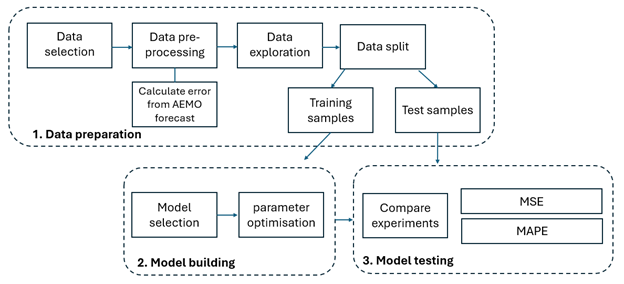
\includegraphics[width=1\linewidth,height=0.3\textheight]{images/MaterialMethods} \caption{Project structure followed to address the research question}\label{fig:modelDiagram}
\end{figure}

\section{Software}\label{software}

Python was the primary software used for data analysis and modelling based on its flexibility in data visualisations and ability to execute machine learning models.

\bigskip

To ensure reproducibility, RMarkdown was used to prepare the final report. Power BI was also used in initial data exploration to understand high-level trends in the data. A Github repository was used to store data, code and working documents. The repository can be found here: \url{https://github.com/unswnick/project}. All relevant code for this project can be found in the Appendices. Appendix A contains data processing code, Appendix B contains Modelling code, and Appendix C contains code for plots.

\bigskip

A summary of software used as part of the project is summarised in Table \ref{tab:tab1}.
\bigskip

\begin{table}[H]
\caption{Summary of software used}
\begin{center}
\begin{tabular}{|l|l|p{19em}|}
\hline
\textbf{Software} & \textbf{Library(s)} & \textbf{Purpose} \\
\hline
\multirow{4}{4em}{Python} & Pandas & Reading, manipulating, cleaning and analysing datasets. \\
\cline{2-3}
& Numpy & Manipulating data and mathematical \newline calculations. \\
\cline{2-3}
& Matplotlib, Seaborn & Visualising data to understand trends and \newline patterns. \\
\cline{2-3}
& Scikit-learn & Implementing and evaluating machine learning algorithms. \\
\hline
PowerBI & - & Summarising and visualising data. \\
\hline
RMarkdown & - & Writing final report. \\
\hline
Github & - & Repository for project documents \\
\hline
\end{tabular}
\end{center}
\label{tab:tab1}
\end{table}

\section{Description of the Data}\label{description-of-the-data}

Table \ref{tab:tab2} describes the data that was used in analysis. In addition to the data files provided by the client, historical weather forecasts including temperature, humidity and wind speed were sourced from OpenWeather (OpenWeather, 2025), a global company specialising in environmental data products. Forecast weather data rather than actual weather data was used as an input to ensure the forecast models were realistic.

\begin{table}[H]
\caption{Datasets used in this project and their properties}
\centering
\begin{tabular}{|p{13em}|p{20em}|}
\hline
\textbf{Data} & \textbf{Description} \\
\hline
\textbf{Electricity demand}\newline Use for both training and testing models. & Electricity demand from 2010 to 2021. Well-structured and low complexity with no duplicates and no null values.\newline Variables: Date-time, totalDemand, regionID\newline
Format: CSV, Storage: Github, Size: 6 Mb, Rows: 196,513 \\
\hline
\textbf{Forecast demand} \newline Used as a baseline forecast model and improve on. & Provides forecasted demand data from 2010 to 2021. Well-structured with no null values. It is high complexity due to uneven time increments and duplicate rows. \newline Variables: Date-time, forecastDemand, totalDemand, regionID, preDispatchSeqNo, periodID, lastChange\newline Format: CSV, Storage: Github, Size: 722 Mb, Rows: 10,906,019 \\
\hline
\textbf{Forecast weather indicators}\newline Exogenous variables included in modelling. & Provides previous forecast weather data for Bankstown from October 7 2017. Well-structured with no null values. \newline Variables: Date-time, temperature, humidity, wind speed, rain\newline Format: CSV, Storage: GitHub, Sharepoint/Teams, Size: 1327.1 MB, Rows: 10854100 \\ 
\hline
\end{tabular}
\label{tab:tab2}
\end{table}

\section{Data Cleaning}\label{data-cleaning}

Data was found to be complete for Electricity Demand data Some forecast data were missing for forecast intervals \textgreater12 hours. To ensure complete data was used, and to reduce computational complexity, the forecast models were trained and tested on 12 hour forecast intervals only. There were no missing values in the Forecast Weather Indicators data, however the available data begins on October 7 2017. Consequently, the relevant data used to train and test the forecast model was between October 7 2017 and 17 March 2021 with a 12 hour forecast interval. No further missing values were present in the data.

\bigskip

Outliers were not removed from the data to ensure data completeness and to avoid introducing bias through exclusions. Further advice from industry experts would be required to determine which outliers, if any, should be removed based on appropriate criteria.

\bigskip

Additional data cleaning steps performed on all datasets are detailed below:

\begin{enumerate}
\def\labelenumi{\arabic{enumi}.}
\item
  Date/time variables were formatted consistently (i.e.~d/m/y H:M)
\item
  Date/time variables were rounded to the nearest 30 minute increment to provide consistent 30-minute intervals
\item
  Duplicate date/time rows were removed to ensure each date/time row was unique
\end{enumerate}

\bigskip

After each dataset was cleaned and checked, they were merged into one clean dataset, joined on the unique date/time variable.

\section{Data pre-processing}\label{data-pre-processing}

Outlined below are the steps undertaken to pre-process the data:

\begin{enumerate}
\def\labelenumi{\arabic{enumi}.}
\item
  \textbf{Feature extraction} -- The following features were extracted from date/time variables:

  \begin{itemize}
  \tightlist
  \item
    Hour\_of\_day
  \item
    Month\_of\_year
  \item
    Day\_of\_week
  \end{itemize}
\item
  \textbf{Label enconding} -- Hour\_of\_day, Day\_of\_week and Month\_of\_year variables were one-hot-encoded into binary variables
\item
  \textbf{Feature engineering} -- The following new features were created:

  \begin{itemize}
  \tightlist
  \item
    Forecast interval (date/time future -- date/time current)
  \item
    Forecast error (total demand -- forecast demand)
  \item
    24-hour Forecast Error (Forecast error from 24 hours ago)
  \item
    48-hour Forecast Error (Forecast error from 48 hours ago)
  \item
    72-hour Forecast Error (Forecast error from 72 hours ago)
  \item
    7-day Forecast Error (Forecast error from 7 days ago)
  \item
    14-day Forecast Error (Forecast error from 14 days ago)
  \item
    Relative error (Forecast error / total demand)
  \item
    Hour × Temperature (Hour * Temperature)
  \item
    Hour (Sine) (hour\_sin) --- sin(2π × Hour / 24)
  \item
    Hour (Cosine) (hour\_cos) --- cos(2π × Hour / 24)
  \item
    Month × Temperature (MonthNumb * Temperature)
  \item
    Hour × Forecast Demand (Hour * forecast\_demand)
  \item
    Temperature × Forecast Demand (Temperature * forecast\_demand)
  \item
    Temperature × Hour (Sine) (Temperature * hour\_sin)
  \item
    Temperature × Hour (Cosine) (Temperature * hour\_cos)
  \item
    Forecast Demand × Hour (Sine) (forecast\_demand * hour\_sin)
  \item
    Forecast Demand × Hour (Cosine) (forecast\_demand * hour\_cos)
  \item
    24-hour Forecast Error × Hour (Cosine) (24hrpreverrors * hour\_cos)
  \item
    24-hour Forecast Error × Hour (Sine) (24hrpreverrors * hour\_sin)
  \end{itemize}
\item
  \textbf{Splitting the data} - As a final step in pre-processing, the data were split into 70\% training 7 October 2017 -- 5 March 2020) and 30\% testing (6 March 2020 -- 17 March 2021). This split allowed for a large number of data to be trained on, and a full year to test which captured all seasonal effects. The same split was used across the models.
\end{enumerate}

Note that modelling methods chosen did not require normalisation of the data.

\section{Assumptions}\label{assumptions}

\begin{itemize}
\item
  AEMO's forecast data is released every 5 minutes, therefore forecast data for the 12 hour interval is available to use in the model
\item
  Temperature/weather forecasts are available for 12 hours into the future.
\item
  Bankstown weather variables are reasonable representations of weather conditions across New South Wales.
\end{itemize}

\section{Modelling Methods}\label{modelling-methods}

The following methods were in this study:

\begin{itemize}
\item
  Linear Regression: Baseline model for improving forecasts due to its simple implementation and interpretability.
\item
  SARIMA: EDA identified autocorrelation between forecast errors. Due to the seasonal nature of electricity demand, SARIMA modelling was conducted.
\item
  Decision Trees: EDA identified non-linearity between electricity demand and its explanatory variables. As such, decisions trees were implemented to explore simpler non-linear behaviors.
\item
  XGBoost: Implemented to explore non-linear behaviors using advanced techniques.
\end{itemize}

These modelling methodologies are described below.

\bigskip

\noindent \textbf{ARIMA}

\bigskip

\noindent Auto Regressive Integrated Moving Average (ARIMA) is a time series forecasting model. Besides being well-researched and more readily explainable compared to machine learning models, its algorithm specifications make it suitable for energy demand forecasting. The model consists of three main components:

\bigskip

Auto Regression: The model utilises lagged observations or previous time points. Due to the weather conditions of previous days having a direct influence on future weather, previous time points are relevant for forecasting. In addition, energy demand also exhibits seasonality that can be captured by previous inputs.

\bigskip

Differencing (Integration): Energy and weather demands over different time horizons exhibit slight trend. Raw observations are differenced to make statistical properties (such as mean or variance) stabilised over time.

\bigskip

Moving average: Smooths variance by modelling a moving average of lagged variables against point residuals. This reduces noise in highly variable factors susceptible to measurement error like weather.

\bigskip

Seasonal Auto Regressive Intergrated Moving Average (SARIMA) is an extension of the ARIMA model. SARIMA is designed to support seasonality in time series data. It can be modified to incorporate seasonality in different time horizons such as weekly, monthly, or quarterly time frames. The model parameters are the same as ARIMA with the inclusion of seasonal variants to control for seasonal effects: seasonal autoregressive order, seasonal differencing order, and seasonal moving average order.

\bigskip

\noindent \textbf{Decision Trees}

\bigskip

\noindent Decision Trees are a type of explainable machine learning model. They are trained by recursively dividing the dataset into subsets using entropy (a measure of impurity or randomness in the dataset) and optimise for information gain. The impurity is in context to the target variable. When a subset of data is comprised of an entire class, it is considered pure. It is interpretable because the model construction can be read as a series of conditional IF statements to achieve certain outputs.

\bigskip

A Random Forest is a collection of generated Decision Trees. The generation formula is consistent across each decision tree, the difference being each tree is generated from a different bootstrap sample. The prediction outputs for regression tasks, such as energy demand forecasting, is an average of all decision tree outputs. Random Forests lose the ability of decision trees to be interpretable, the benefit however, is improved accuracy and robustness.

\bigskip

\noindent \textbf{XGBoost}

\bigskip

\noindent XGBoost, short for extreme gradient boosting, is a gradient descent machine learning method. Its formulation is by use of a loss function to measure the difference between predicted and actual values and a regularization term to penalize complex models.

\bigskip

It functions by building decision trees sequentially. Each tree is trained to predict the residuals from previous trees. Each tree split mechanism follows the process of regular decision tree training. Each tree's contribution to the final prediction is weighted by a learning rate. It generally outperforms regular decision tree models due to its internal corrections of error and feature selection. Its construction makes it suitable for regression tasks such as energy demand forecasting.

\chapter{Exploratory Data Analysis}\label{exploratory-data-analysis}

This section presents an exploratory analysis of the temperature, forecasted demand, and actual electricity demand data. Exploratory data analysis (EDA) explored how demand responds to temperature variations and where forecast discrepancies are most pronounced. The data is manipulated and visualised with Python.

\bigskip

We begin the analysis by focusing on the individual distributions and characteristics of each dataset. This stage provides context on the seasonal variability of the data.

\section{Electricity Demand}\label{electricity-demand}

Electricity demand shows a cyclical pattern with a downward trend when observing it throughout the years (Figure \ref{fig:yeardemand}). This may be due to more households investing in embedded generation to supplement their electricity supply.

\begin{figure}
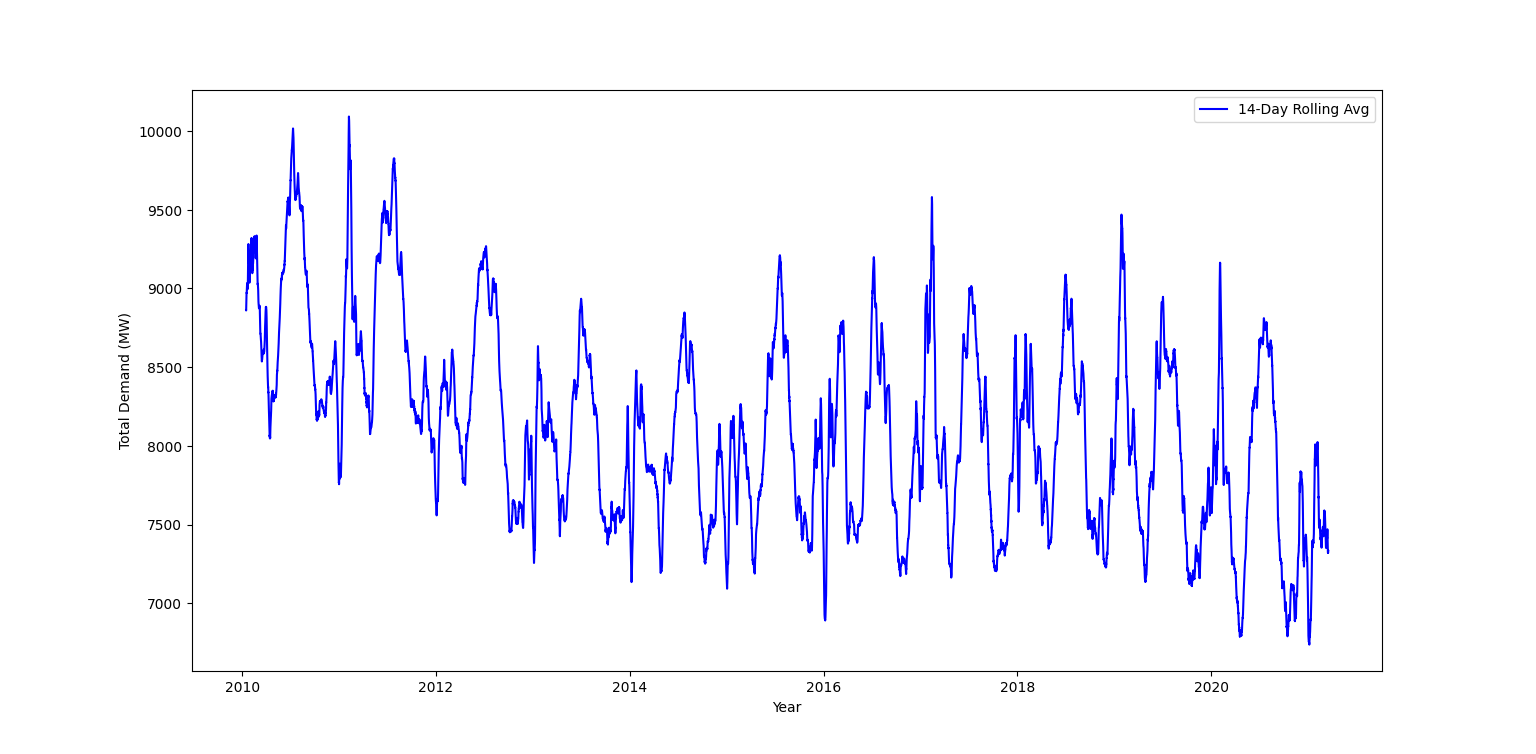
\includegraphics[width=1\linewidth,height=0.4\textheight]{images/demandvtime} \caption{Electricity Demand vs Time}\label{fig:yeardemand}
\end{figure}

Electricity demand is higher during winter and summer months (Figure \ref{fig:monthdemand}). This is likely due to higher consumption of electricity to power heating and cooling appliances.

\begin{figure}
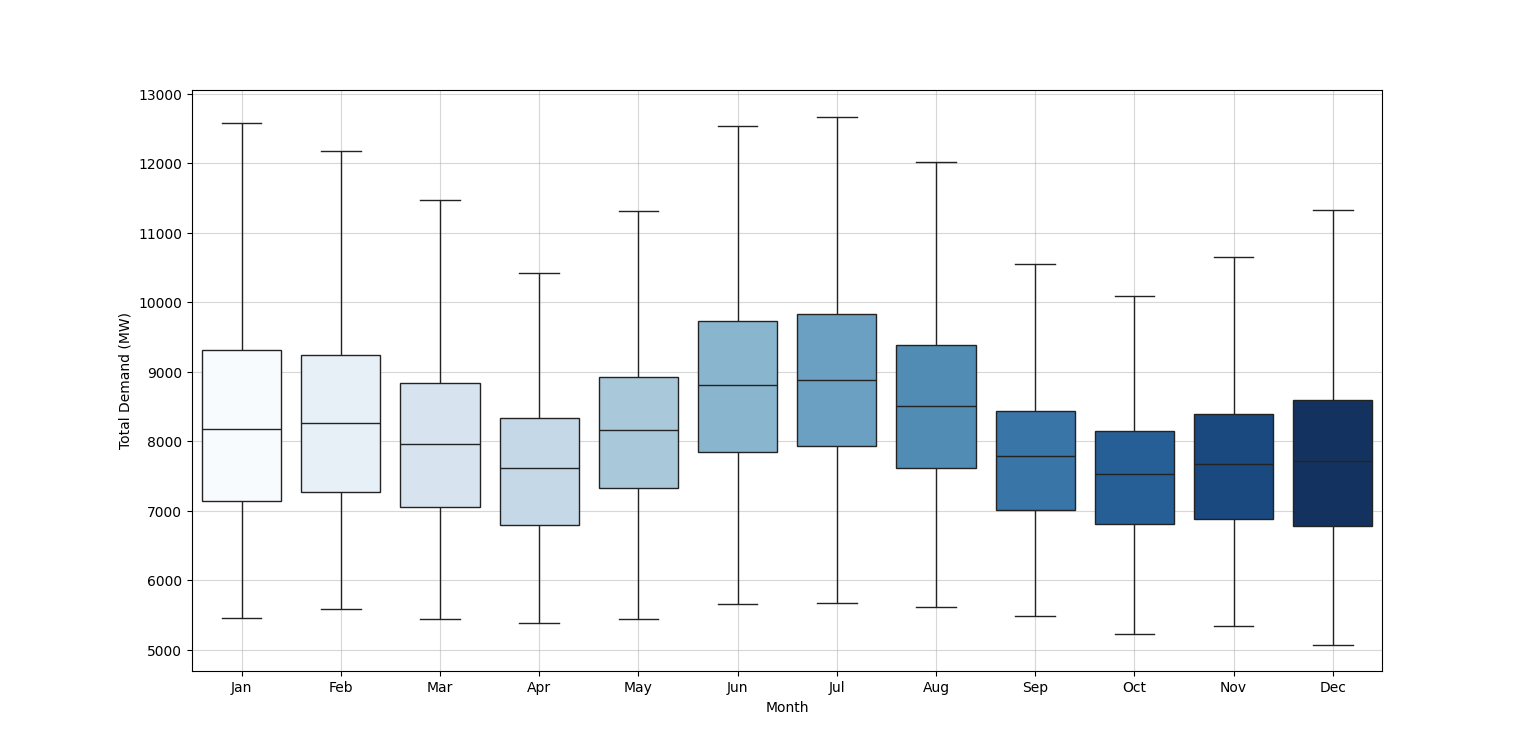
\includegraphics[width=1\linewidth,height=0.4\textheight]{images/demandMonth} \caption{Total Demand by Month}\label{fig:monthdemand}
\end{figure}

Demand was observed to be greater in weekdays than weekends (Figure \ref{fig:weekdemand}). This may be due to many businesses closing during weekends.

\begin{figure}
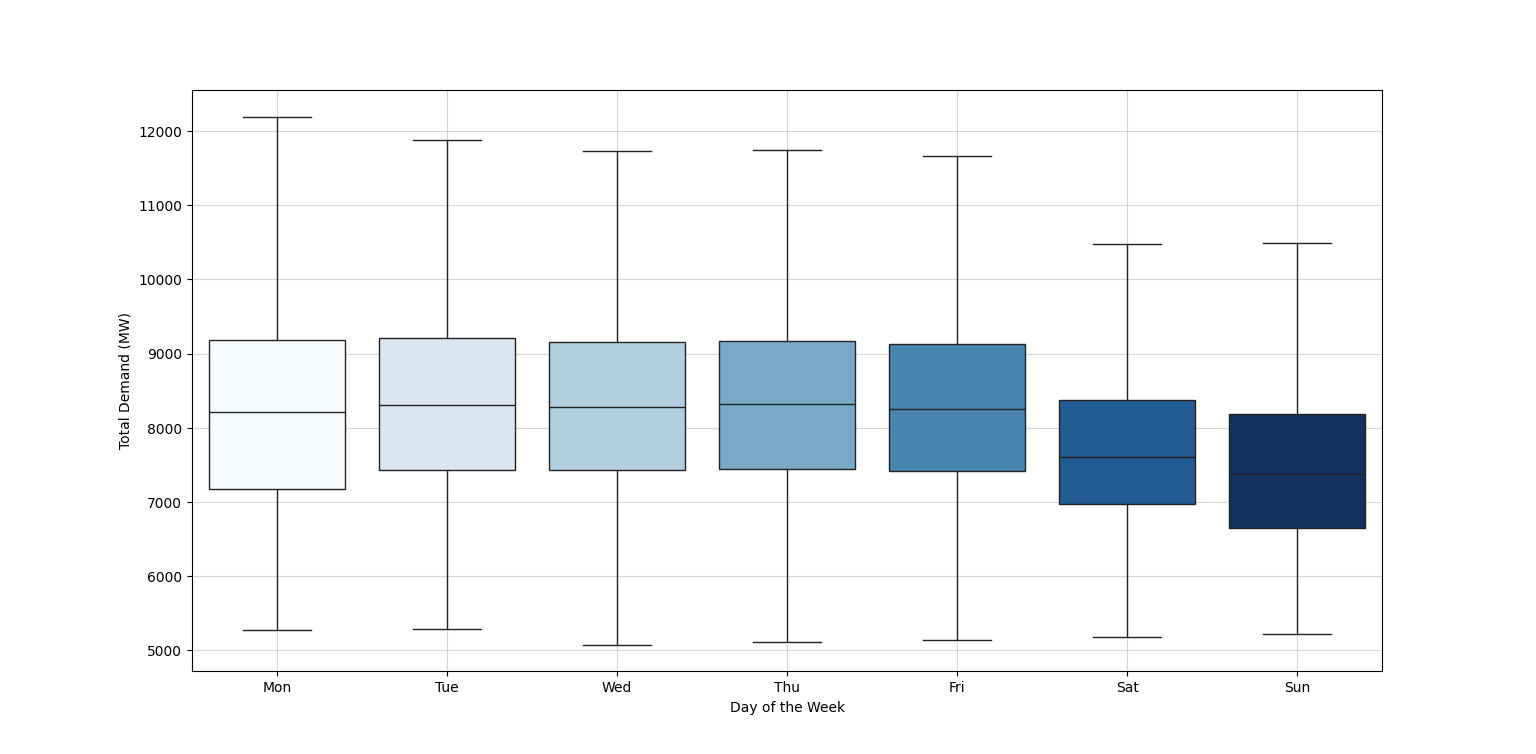
\includegraphics[width=1\linewidth,height=0.4\textheight]{images/WeekDemand} \caption{Total Demand by Day of the Week}\label{fig:weekdemand}
\end{figure}

Electricity demand is relatively high between 8am and 11pm (Figure \ref{fig:hourdemand}), likely due to the human sleeping cycle.

\begin{figure}
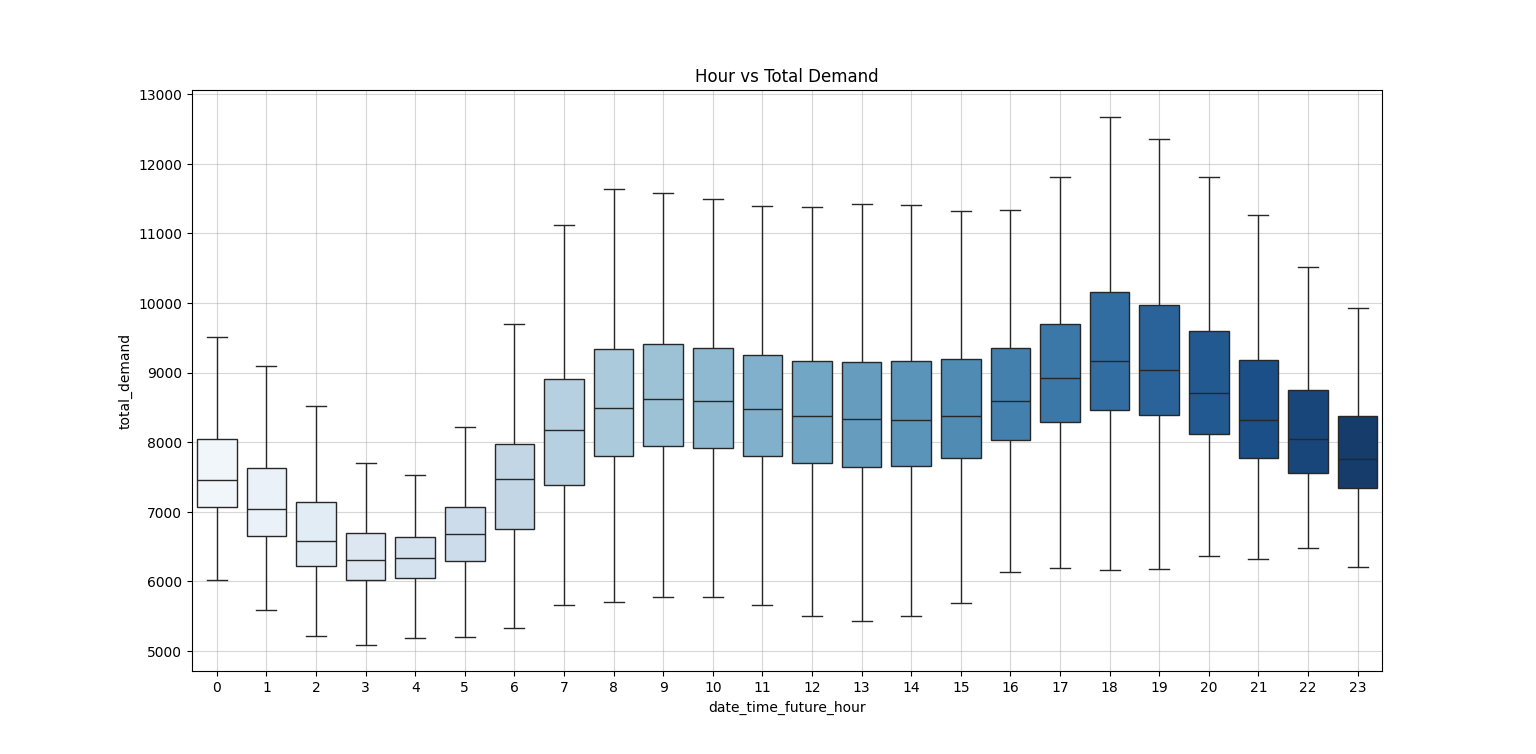
\includegraphics[width=1\linewidth,height=0.3\textheight]{images/demandHour} \caption{Total Demand by Hour of Day}\label{fig:hourdemand}
\end{figure}

\section{Forecast Electricity Demand}\label{forecast-electricity-demand}

This dataset contains electricity demand forecasts made every 30 minutes. Each time a forecast is made, it includes 48 predictions---one for each half-hour period from 30 minutes ahead up to 24 hours ahead.

\bigskip

The scatter plot of electricity demand forecasts vs actual electricity demand across different prediction time periods (Figure \ref{fig:forecastdem}), reveals lower correlation as both the prediction time period and actual electricity demand increase.

\begin{figure}
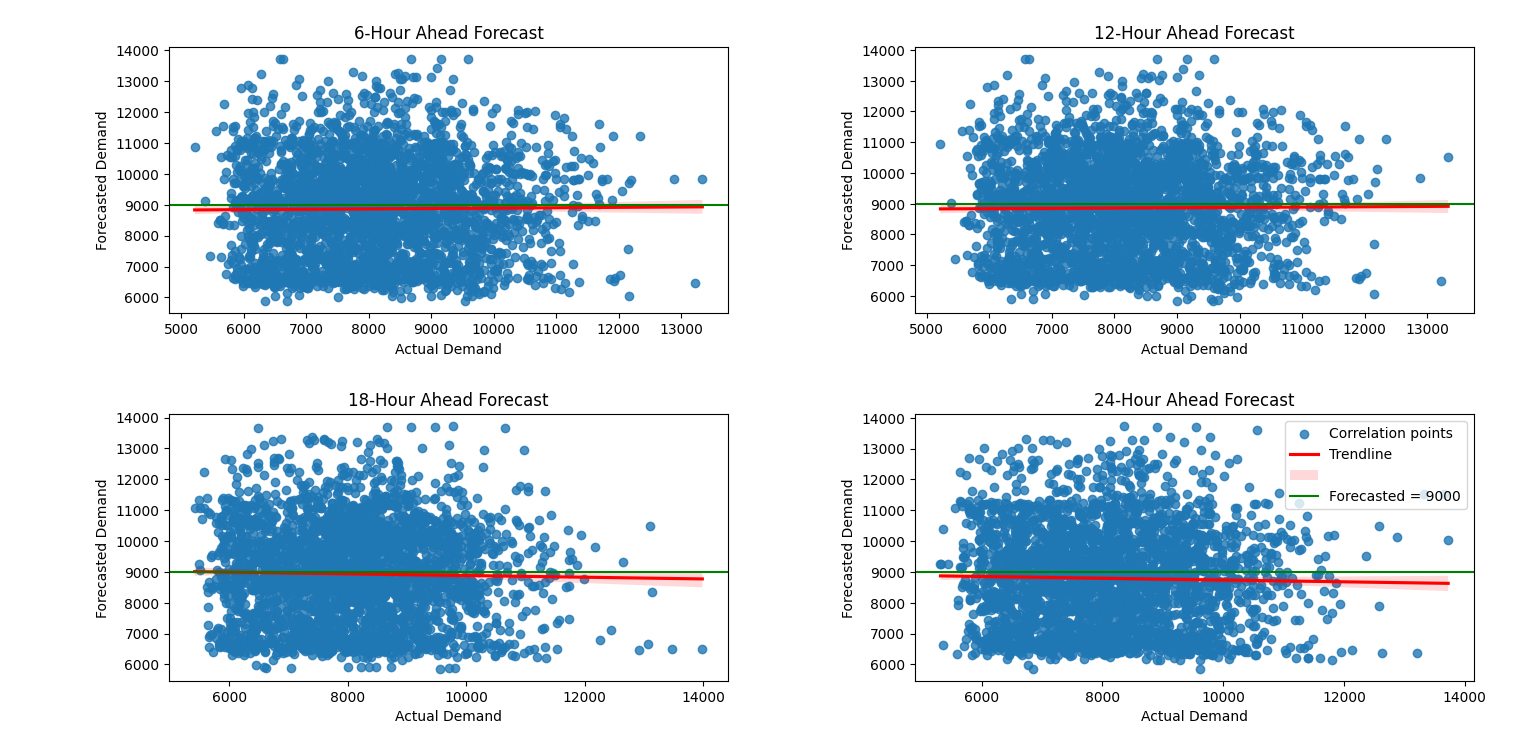
\includegraphics[width=1\linewidth,height=0.4\textheight]{images/forecastdemscatter} \caption{Scatter plots of Forecast Demand vs Total Demand by Lag interval}\label{fig:forecastdem}
\end{figure}

\section{Weather Variables vs Electricity Demand}\label{weather-variables-vs-electricity-demand}

In this next section, we will examine if and how weather affects both the electricity demand and its forecast.

\bigskip

The correlation of relevant weather variables with electricity demand shows weak correlation across all variables, with humidity having the highest correlation and rain having the lowest (Figure \ref{fig:weatherdemand}).

\begin{figure}
\includegraphics[width=1\linewidth,height=0.3\textheight]{images/WeatherVDemand} \caption{Correlation of Weather variables with Electricity Demand}\label{fig:weatherdemand}
\end{figure}

The plot of temperature against electricity demand reveals a distinct U-shaped correlation. This pattern reflects energy usage behaviour in response to extreme temperatures (Figure \ref{fig:tempcorr}). The lowest demand levels generally occur in temperate conditions where neither heating nor cooling is heavily used.

\begin{figure}
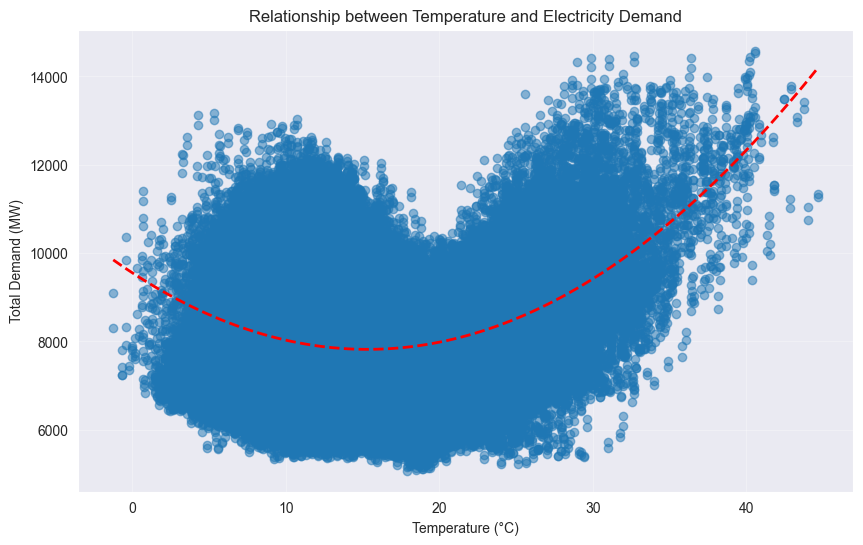
\includegraphics[width=1\linewidth,height=0.35\textheight]{images/tempvsdemand} \caption{Scatter plot of Electricity demand vs Temperature}\label{fig:tempcorr}
\end{figure}

\section{Forecast Error of Electricity Demand}\label{forecast-error-of-electricity-demand}

In this section, we will explore whether forecast inaccuracies are correlated with known variables which contribute to electricity demand. Forecast error was defined as actual demand less forecast demand.

\bigskip

Figure \ref{fig:errorvtemp} shows that forecast error increases with temperature for temperatures greater than \textasciitilde29°C. This suggests the current forecasting model may lack information regarding forecasted temperatures. The trend also occurs for normalised demand (Figure \ref{fig:relerrorvtemp}).

\begin{figure}
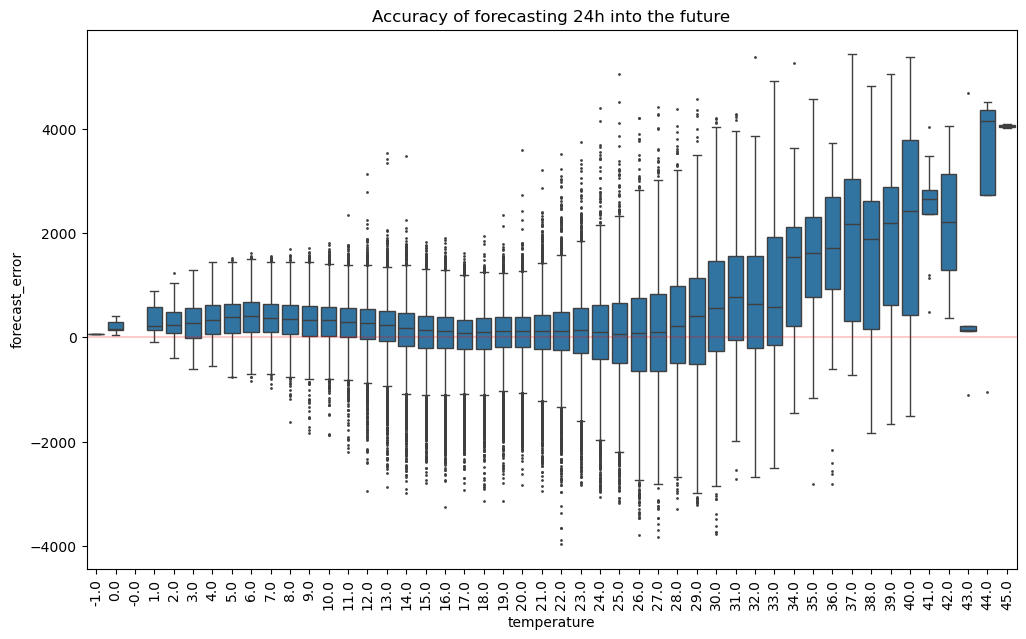
\includegraphics[width=1\linewidth,height=0.4\textheight]{images/forecastErrorTemp} \caption{Forecast Error vs Temperature Forecast}\label{fig:errorvtemp}
\end{figure}

\begin{figure}
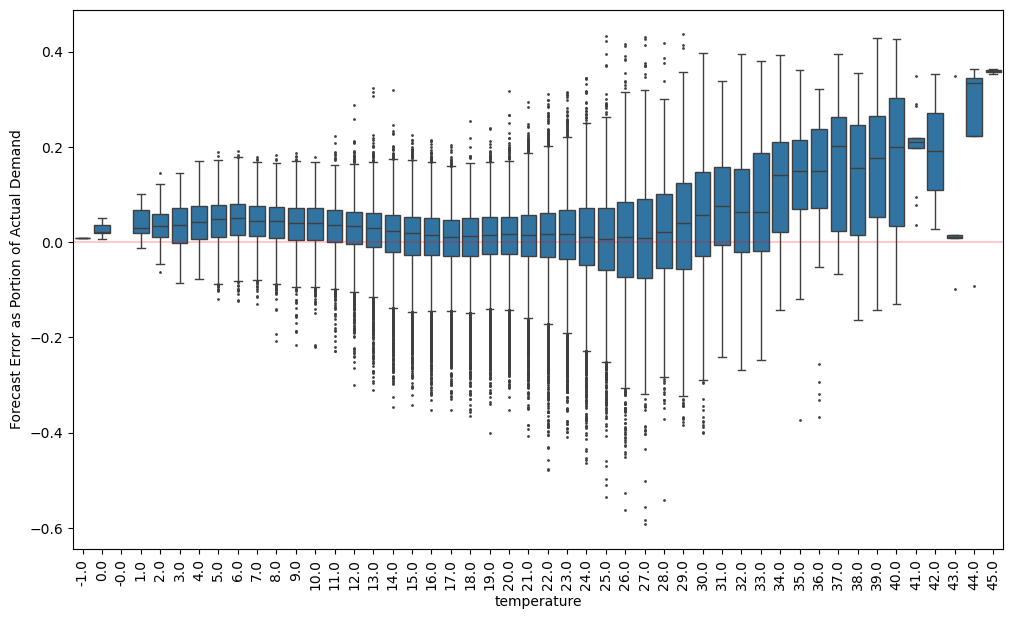
\includegraphics[width=1\linewidth,height=0.4\textheight]{images/PortionErrorTemp} \caption{Normalised forecast error vs temperature forecast}\label{fig:relerrorvtemp}
\end{figure}

\subsection{Time Series Analysis}\label{time-series-analysis}

Time series analysis of the forecast error was conducted to understand whether errors persisted with time. It was conducted for 6, 12, 18 and 24-hour forecasts.

\bigskip

Augmented Dickey-Fuller test (ADF Test) was conducted. It showed significant evidence for stationary forecast errors (Table \ref{tab:tab3}).

\begin{table}[H]
\caption{ADF tests conducted for 6, 12, 18 and 24-hour forecasts}
\centering
\begin{tabular}{||c||c||}
\hline
Hour of day = 6 & Hour of Day = 18 \\
\hline
ADF Statistic: -33.863838 & ADF Statistic: -31.926828 \\
p-value: 0.000000 & p-value: 0.000000 \\
Critical Values: & Critical Values: \\
 1\%: -3.430  &  1\%: -3.430 \\
 5\%: -2.862 &   5\%: -2.862 \\
 10\%: -2.567 &  10\%: -2.567 \\
Stationary & Stationary \\
\hline
\hline
Hour of Day = 12 & Hour of Day = 24 \\
\hline
ADF Statistic: -33.407029 & ADF Statistic: -29.030458 \\
p-value: 0.000000 & p-value: 0.000000 \\
Critical Values: & Critical Values: \\
 1\%: -3.430 &  1\%: -3.430 \\
 5\%: -2.862 &  5\%: -2.862 \\
 10\%: -2.567 &  10\%: -2.567 \\
Stationary & Stationary \\
\hline
\end{tabular}
\label{tab:tab3}
\end{table}

Autocorrelation function (ACF) and partial autocorrelation function (PACF) plots were generated to understand the relationship between forecast errors and lagged versions of itself over successive time lags (Figure \ref{fig:acfErrors}, Figure \ref{fig:pacfErrors}). PACF plots showed that forecast errors were significantly partially correlated with the most recent forecasts and ones made 24 and 48 hours prior. The partial correlation of the 24-hour lagged forecast error was of note due its greater significance than the 48-hour lag and its availability when forecasting.

\begin{figure}
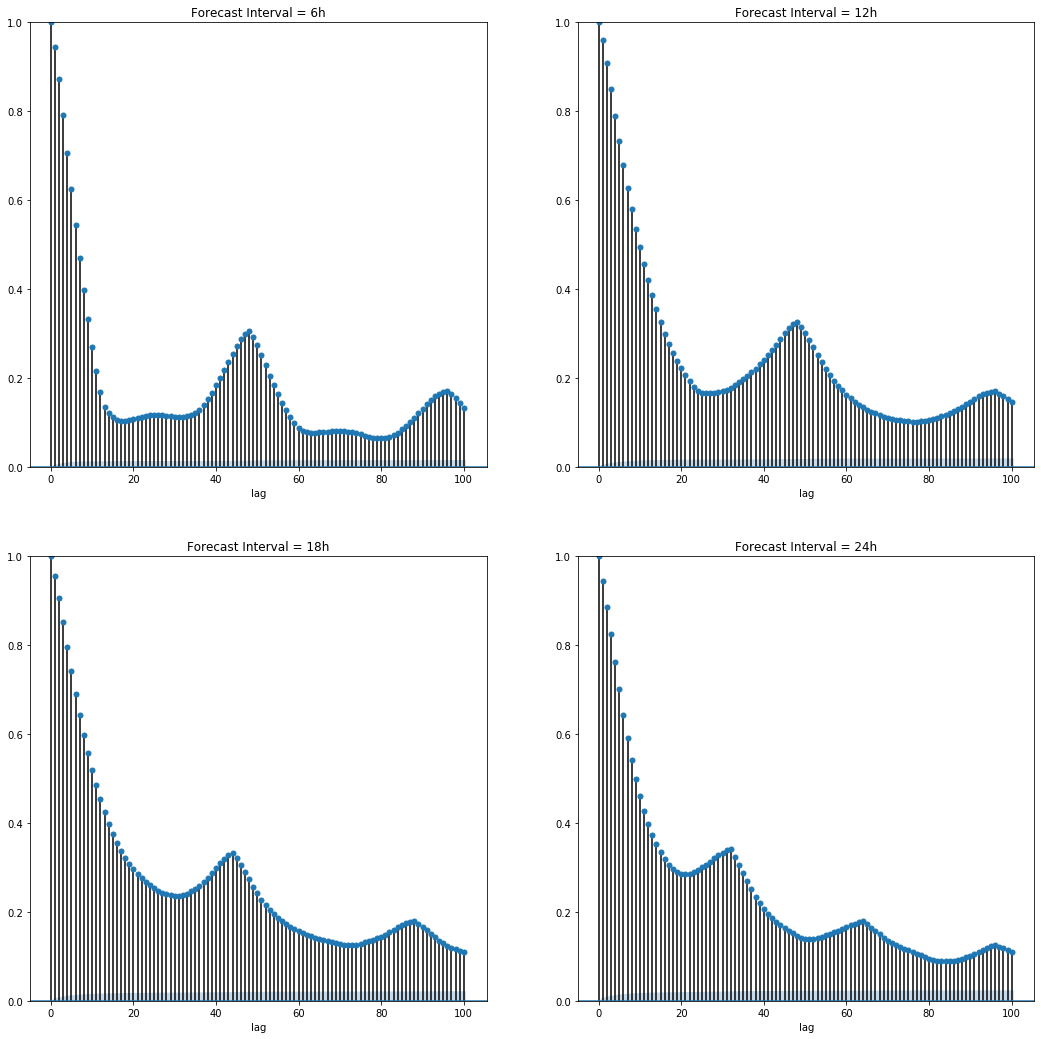
\includegraphics[width=1\linewidth,height=0.65\textheight]{images/ACFForecastErrors} \caption{ACF of forecast errors}\label{fig:acfErrors}
\end{figure}

\begin{figure}
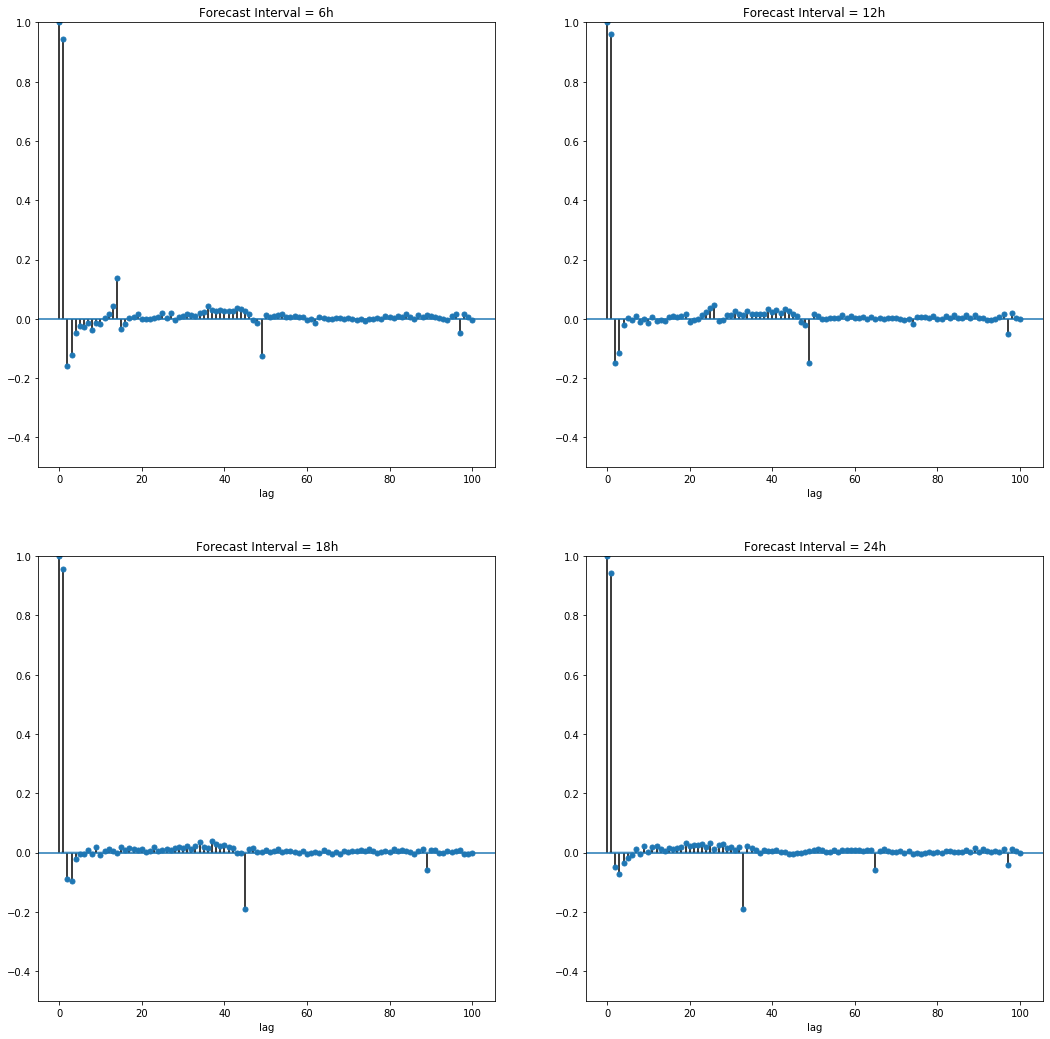
\includegraphics[width=1\linewidth,height=0.6\textheight]{images/PACFForecastErrors} \caption{PACF of forecast errors}\label{fig:pacfErrors}
\end{figure}

Scatterplots and correlations for forecast errors and its 24-hour lagged error can be seen in Figure \ref{fig:laggedError}.

\begin{figure}
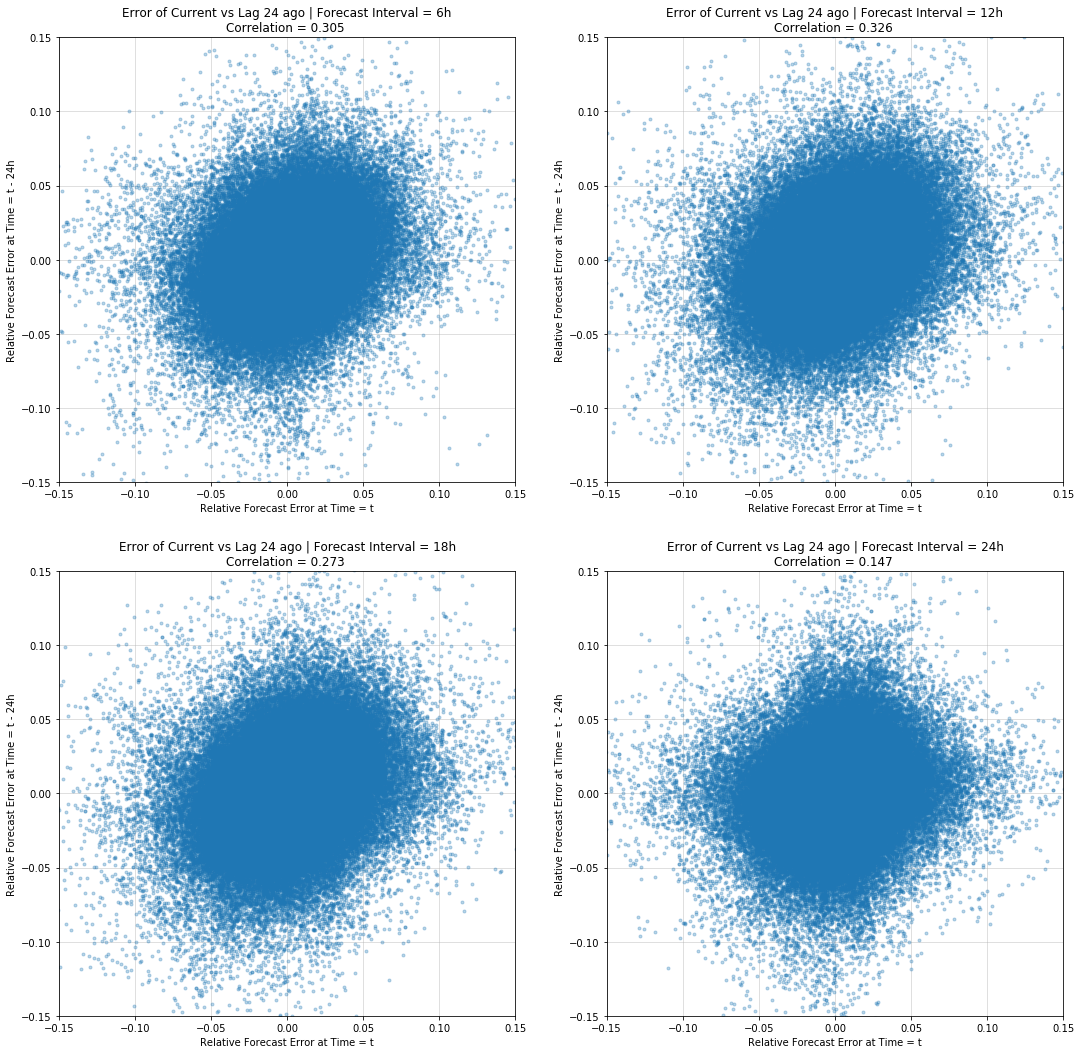
\includegraphics[width=1\linewidth,height=0.6\textheight]{images/ForecastErrorCorrelations} \caption{Scatterplots and correlations for forecast errors and its 24-hour lagged errors}\label{fig:laggedError}
\end{figure}

\section{Summary of Key Findings}\label{summary-of-key-findings}

\begin{itemize}
\item
  \textbf{U-shaped relationship between temperature and electricity demand:} Electricity demand increases during both extreme cold and extreme heat conditions, with the lowest demand observed during temperate conditions. This pattern is consistent with expected heating and cooling behavior and is evident in both actual and forecasted demand data.
\item
  \textbf{Forecasting models capture seasonal trends:} Forecasted electricity demand shows a similar U-shaped relationship with temperature, indicating that the models are aligned with seasonal usage patterns.
\item
  \textbf{Forecast error increases non-linearly with temperature, especially during extreme heat:} Forecast accuracy deteriorates significantly at higher temperatures, suggesting that current models underperform during periods of extreme heat. In comparison, performance during extreme cold is better, though still less accurate than under mild conditions.
\item
  \textbf{Forecast errors are autocorrelated with past errors:} Forecast errors may be modelled by understanding historical forecast errors. Of note, the 24-hour lagged forecast error may be used for improving forecasts.
\item
  \textbf{The forecast has the potential to be improved:} These findings highlight some correlations between forecast errors, temperature and time variables such as season which may indicate the model could be improved by modelling forecast errors.
\end{itemize}

\chapter{Analysis and Results}\label{analysis-and-results}

\section{Performance measures}\label{performance-measures}

Two common performance measures were chosen to calculate prediction accuracy and compare models. Mean square error (MSE) and mean absolute percentage error (MAPE) were chosen to be the most appropriate measures. MSE penalises large errors which is useful to assess when the aim is to reduce large errors. Furthermore, MAPE provides an easily interpretable and comparable result. The measures are described below:

\bigskip

MSE is the average of the squared difference between actual demand and forecasted demand.

\begin{equation*}
\text{MSE} = \frac{1}{n}\sum^{n}_{i=1}{(Y_i-{\hat{Y}_{i}})^2}
\end{equation*}

MAPE takes the absolute value of the difference between the actual demand and forecast demand expresses it as a percentage of actual demand, and takes the average of this.

\begin{equation*}
\text{MAPE} = \frac{1}{n}\sum^{n}_{i=1}{\frac{\lvert A_{i}-F_{i}\rvert}{A_{i}} * 100}
\end{equation*}

For both measures, a smaller value represents higher accuracy, and a better performing model.

\bigskip

MSE and MAPE values for the original forecast can be seen below.

\begin{align*}
\text{Existing model MSE} &= 55159 \\
\text{Existing model MAPE} &= 2.19\% \\
\end{align*}

\section{Linear Regression}\label{linear-regression}

Forecast error was defined as actual demand less forecast demand (Equation \eqref{eq:oneA}).

\begin{equation}
\varepsilon_t = y_t - \hat{y}_{t} \label{eq:oneA}
\end{equation}

Two linear regression models were trained for predicting the forecast error (Equation \eqref{eq:oneB}). The predicted forecast error was then used to update the forecast (Equation \eqref{eq:oneC}). The aim of the models was to reduce the updated forecast error (i.e.~\(\varepsilon^{*}_t < \varepsilon\)).

\begin{equation}
\varepsilon_t = \hat{\varepsilon}_t(...) + \varepsilon^{*}_t \label{eq:oneB}
\end{equation}

\begin{equation}
\hat{y}^{*}_{t} = \hat{y}_t + \hat{\varepsilon}_{t}(...) + \varepsilon^{*}_t \label{eq:oneC}
\end{equation}

\subsection{Model Construction}\label{model-construction}

\bigskip

\textbf{Linear Regression - Model 1}
\bigskip

\noindent The first model used only the 24-hour lag forecast error for predicting the forecast error (Equation \eqref{eq:oneD}). Hence, it was a simple autoregressive model.

\begin{equation}
\varepsilon^{\text{(LR1)}}_t = \theta_{0} + \theta_{1}\varepsilon_{t-24h} \label{eq:oneD}
\end{equation}

The model summary can be seen in Table \ref{tab:tab4}. It showed that all variables are significant at the 0.05 significance level.
\bigskip

\begin{table}[H]
\caption{Linear Regression Model 1, OLS Regression Results}
\centering
\begin{tabular}{lr|lr}
\hline
\hline
\multicolumn{4}{c}{OLS Regression Results} \\
\hline
\hline
Dep. Variable: & y & R-squared: & 0.113 \\
Model: & OLS & Adj. R-squared: & 0.113 \\
Method: & Least Squares & F-statistic: & 2696. \\
Date: & Sun, 20 Apr 2025 & Prob (F-statistic): & 0.00 \\
Time: & 11:19:06 & Log-Likelihood: & -1.4233e+05 \\
No. Observations: & 21064 & AIC: & 2.847e+05 \\
Df Residuals: & 21062 & BIC: & 2.847e+05 \\
Df Model: & 1 & & \\                                         
Covariance Type: & nonrobust & & \\
\hline
\hline
\end{tabular}

\begin{tabular}{lrrrrrr}
  & coef & std err & t & P>|t| & [0.025 & 0.975] \\
\hline
const & 10.5613 & 1.438 & 7.346 & 0.000 & 7.743 & 13.379 \\
forecast\_error & 0.3369 & 0.006 & 51.927 & 0.000 & 0.324 & 0.350 \\
\hline
\hline
\end{tabular}

\begin{tabular}{lrlr}
Omnibus: & 2737.590 & Durbin-Watson: & 0.201 \\
Prob(Omnibus): & 0.000 & Jarque-Bera (JB): & 23155.543 \\
Skew: & -0.344 & Prob(JB): & 0.00 \\
Kurtosis: & 8.090 & Cond. No. & 222.\\
\hline
\hline
\end{tabular}
\label{tab:tab4}
\end{table}

\noindent \textbf{Linear Regression - Model 2}

\bigskip

\noindent The second model used the 24-hour lag forecast error and all possible explanatory variables for the forecast error identified in EDA (Equation \eqref{eq:oneE}).

\begin{equation}
\begin{split}
\varepsilon^{(LR2)}_{t} = &\theta_0 + \theta_1\varepsilon_{t-24h} +\theta_{2}forecastTemperature_t + \\
& \theta_{3}forecastHumidity_t + \theta_{4}forecastWind_t + \theta_{5}forecastRain_t + \\
& \theta_{6}isSaturday_t + \theta_{7}isSunday_t + \theta_{8}isJanuary_t + \\
& \theta_{9}isNovember_t + \theta_{10}isDecember_t
\end{split}
\label{eq:oneE}
\end{equation}

The model summary can be seen in Table \ref{tab:tab5}. It showed that all variables, except \textit{forecastRain}, are significant at the 0.05 significance level.

\begin{table}[H]
\centering
\caption{Linear Regression Model 2, OLS Regression Results}
\begin{tabular}{lr|lr}
\hline
\hline
\multicolumn{4}{c}{OLS Regression Results} \\
\hline
\hline
Dep. Variable: & y & R-squared: & 0.124 \\
Model: & OLS & Adj. R-squared: & 0.124 \\
Method: & Least Squares & F-statistic: & 298.6 \\
Date: & Sun, 20 Apr 2025 & Prob (F-statistic): & 0.00 \\
Time: & 11:19:08 & Log-Likelihood: & -1.4220e+05 \\
No. Observations: & 21064 & AIC: & 2.844e+05 \\
Df Residuals: & 21053 & BIC: & 2.845e+05 \\
Df Model: & 10 & & \\                                         
Covariance Type: & nonrobust & & \\
\hline
\hline
\end{tabular}

\begin{tabular}{lrrrrrr}
  & coef & std err & t & P>|t| & [0.025 & 0.975]  \\
\hline
const & 10.5613 & 1.438 & 7.346 & 0.000 & 7.743 & 13.379  \\
forecast\_error & 0.3369 & 0.006 & 51.927 & 0.000 & 0.324 & 0.350 \\
Temperature & -1.1963 & 0.296 & -4.040 & 0.000 & -1.777 & -0.616  \\
Humidity & 0.9220 & 0.094 & 9.811 & 0.000 & 0.738 & 1.106  \\
Wind\_speed & 6.7613 & 0.927 & 7.296 & 0.000 & 4.945 & 8.578  \\
Rain & -3.8983 & 2.807 & -1.389 & 0.165 & -9.399 & 1.603  \\
isSaturday & 29.1366 & 4.143 & 7.033 & 0.000 & 21.016 & 37.257 \\
isSunday & 8.2777 & 4.149 & 1.995 & 0.046 & 0.145 & 16.410  \\
isDecember & 20.6354 & 4.986 & 4.139 & 0.000 & 10.863 & 30.408  \\
isJanuary & 13.2394 & 5.233 & 2.530 & 0.011 & 2.982 & 23.497  \\
isNovember & 10.3352 & 4.832 & 2.139 & 0.032 & 0.865 & 19.805  \\
\hline
\hline
\end{tabular}

\begin{tabular}{lrlr}
Omnibus: & 2701.773 & Durbin-Watson: & 0.203 \\
Prob(Omnibus): & 0.000 & Jarque-Bera (JB): & 23691.264 \\
Skew: & -0.315 & Prob(JB): & 0.00 \\
Kurtosis: & 8.157 & Cond. No. & 1.67e+03\\
\hline
\hline
\end{tabular}
\label{tab:tab5}
\end{table}

\subsection{Model Performance}\label{model-performance}

The predicted forecast error was then used to update the forecast error (Equation \eqref{eq:oneC}. Model evaluation (MSE and MAPE) can be seen below.

\begin{multicols}{2}
\noindent\textbf{LRegression Model 1 Performance} \\
- MSE: 49348 \\
- MAPE: 2.06\% \\


\columnbreak


\noindent\textbf{LRegression Model 2 Performance} \\
- MSE: 49718\\
- MAPE: 2.078\%\\
\end{multicols}

Model 1 performed better as it minimised both MAPE and MSE values.

\section{S-ARIMA}\label{s-arima}

Two SARIMA model collections were trained for predicting the forecast error (Equation \eqref{eq:oneB}. The predicted forecast error was then used to update the forecast (Equation \eqref{eq:oneC}). The aim of the models was to reduce the updated forecast error (i.e.~\(\varepsilon^{*}_{t} < \varepsilon_t\)).

\bigskip

A model collection contained a SARIMA model for each hour of the day. This reduced overall computation time, while allowing hour of day to be an explanatory variable (note, training the model on all data was not feasible due to limited computing power). The large data size should allow for data segmentation to have minimal impact on model training.

\bigskip

EDA, conducted earlier, showed that forecast errors are partially correlated with lagged values of itself in 24-hour intervals. As such, SARIMA modelling only considered lags of 24-hours.

\subsection{Parameter Selection}\label{parameter-selection}

ADF tests conducted showed significant evidence for stationary forecast errors, after segmentation by hour of day (Table \ref{tab:tab6}). As such no differencing (d, D) was considered for SARIMA modelling.

\begin{table}[H]
\caption{ADF tests for 4, 10, 16, 22-hour forecasts}
\centering
\begin{tabular}{||c||c||}
\hline
Hour of day = 4 & Hour of Day = 10 \\
\hline
ADF Statistic: -5.875132 & ADF Statistic: -7.680207 \\
p-value: 0.000000 & p-value: 0.000000 \\
Critical Values: & Critical Values: \\
 1\%: -3.432  &  1\%: -3.432 \\
 5\%: -2.862 &   5\%: -2.862 \\
 10\%: -2.567 &  10\%: -2.567 \\
Stationary & Stationary \\
\hline
\hline
Hour of Day = 16 & Hour of Day = 22 \\
\hline
ADF Statistic: -9.601104 & ADF Statistic: -7.968233 \\
p-value: 0.000000 & p-value: 0.000000 \\
Critical Values: & Critical Values: \\
 1\%: -3.432 &  1\%: -3.432 \\
 5\%: -2.862 &  5\%: -2.862 \\
 10\%: -2.567 &  10\%: -2.567 \\
Stationary & Stationary \\
\hline
\end{tabular}
\label{tab:tab6}
\end{table}

\bigskip

ACF and PACF plots were generated to assist in SARIMA parameters selection (Figure \ref{fig:ACF}, Figure \ref{fig:PACF}). The PACF plot showed that, generally, forecast errors are partially correlated with the first lagged term, followed by the next six lagged term, then 1-week and 2-week lags. As such, auto-regressed parameters (p) considered were 1, 2, 6 and 7, and the auto-regressed seasonal parameters (P) considered were 1 and 2. The seasonality parameter (s) was set at 7 for a weekly seasonality.

\begin{figure}
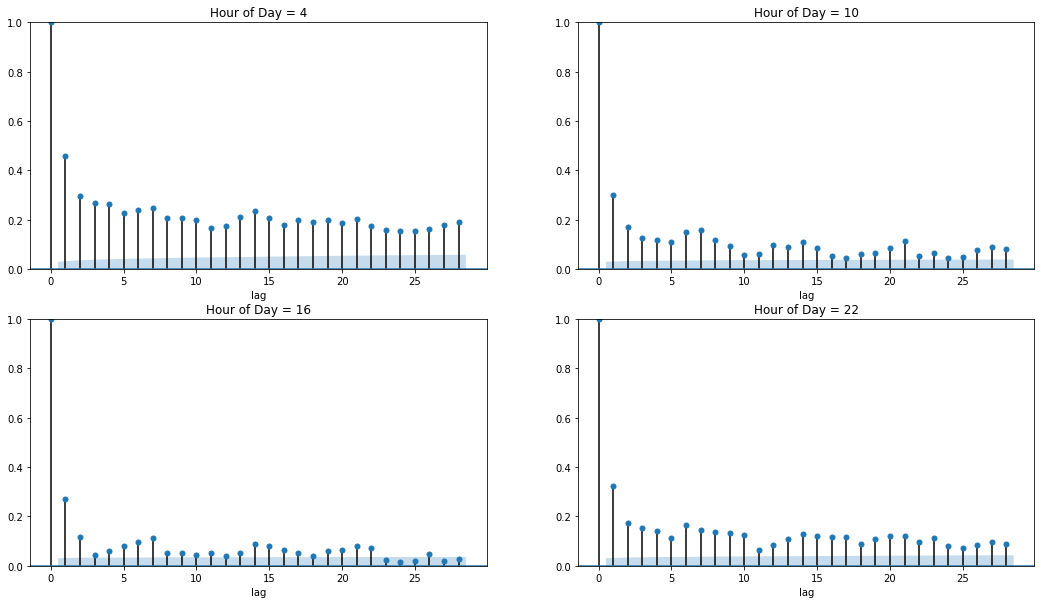
\includegraphics[width=1\linewidth,height=0.35\textheight]{images/Stationarity1} \caption{ACF of forecast errors with 24-hour lags}\label{fig:ACF}
\end{figure}

\begin{figure}
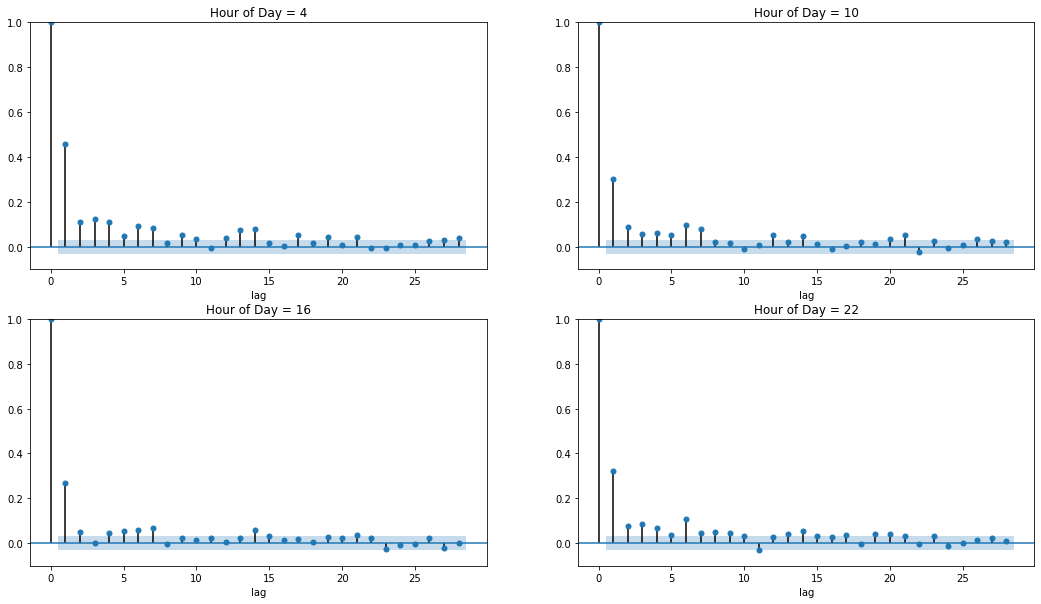
\includegraphics[width=1\linewidth,height=0.35\textheight]{images/Stationarity2} \caption{PACF of forecast errors with 24-hour lags}\label{fig:PACF}
\end{figure}

\bigskip

Moving average parameters considered (q, Q) were 0, 1 and 2. A summary of model parameters can be seen in Table \ref{tab:tab7}.

\bigskip

\begin{table}[H]
\centering
\caption{SARIMA Model parameters}
\begin{tabular}{|c|ccc|cccc|}
\hline
\multirow{2}{*}{\textbf{ID}} & \multicolumn{3}{c|}{\textbf{ARIMA Order}} & \multicolumn{4}{c|}{\textbf{Seasonal Order}} \\ \cline{2-8} 
 & \multicolumn{1}{c|}{\textbf{p}} & \multicolumn{1}{c|}{\textbf{d}} & \textbf{q} & \multicolumn{1}{c|}{\textbf{p}} & \multicolumn{1}{c|}{\textbf{D}} & \multicolumn{1}{c|}{\textbf{Q}} & \textbf{s} \\ \hline
0 & \multicolumn{1}{c|}{1} & \multicolumn{1}{c|}{0} & 0 & \multicolumn{1}{c|}{0} & \multicolumn{1}{c|}{0} & \multicolumn{1}{c|}{0} & 0 \\ \hline
1 & \multicolumn{1}{c|}{1} & \multicolumn{1}{c|}{0} & 1 & \multicolumn{1}{c|}{0} & \multicolumn{1}{c|}{0} & \multicolumn{1}{c|}{0} & 0 \\ \hline
2 & \multicolumn{1}{c|}{7} & \multicolumn{1}{c|}{0} & 1 & \multicolumn{1}{c|}{0} & \multicolumn{1}{c|}{0} & \multicolumn{1}{c|}{0} & 0 \\ \hline
3 & \multicolumn{1}{c|}{7} & \multicolumn{1}{c|}{0} & 7 & \multicolumn{1}{c|}{0} & \multicolumn{1}{c|}{0} & \multicolumn{1}{c|}{0} & 0 \\ \hline
4 & \multicolumn{1}{c|}{1} & \multicolumn{1}{c|}{0} & 0 & \multicolumn{1}{c|}{1} & \multicolumn{1}{c|}{0} & \multicolumn{1}{c|}{1} & 7 \\ \hline
5 & \multicolumn{1}{c|}{6} & \multicolumn{1}{c|}{0} & 2 & \multicolumn{1}{c|}{1} & \multicolumn{1}{c|}{0} & \multicolumn{1}{c|}{1} & 7 \\ \hline
6 & \multicolumn{1}{c|}{6} & \multicolumn{1}{c|}{0} & 2 & \multicolumn{1}{c|}{1} & \multicolumn{1}{c|}{0} & \multicolumn{1}{c|}{2} & 7 \\ \hline
7 & \multicolumn{1}{c|}{8} & \multicolumn{1}{c|}{0} & 1 & \multicolumn{1}{c|}{2} & \multicolumn{1}{c|}{0} & \multicolumn{1}{c|}{1} & 7 \\ \hline
8 & \multicolumn{1}{c|}{2} & \multicolumn{1}{c|}{0} & 1 & \multicolumn{1}{c|}{2} & \multicolumn{1}{c|}{0} & \multicolumn{1}{c|}{1} & 7 \\ \hline
\end{tabular}
\label{tab:tab7}
\end{table}

\bigskip

MSE and MAPE values were generated for each model in Table \ref{tab:tab7} (Figure \ref{fig:MSEsarima}, Figure \ref{fig:MAPEsarima}). Models 5, 6 and 7 equally improved MSE and minimised MAPE values. Model 5 was selected as it was the least complex of the three.

\begin{figure}
\includegraphics[width=1\linewidth,height=0.3\textheight]{images/MSEarima} \caption{MSE improvement for each SARIMA model}\label{fig:MSEsarima}
\end{figure}

\begin{figure}
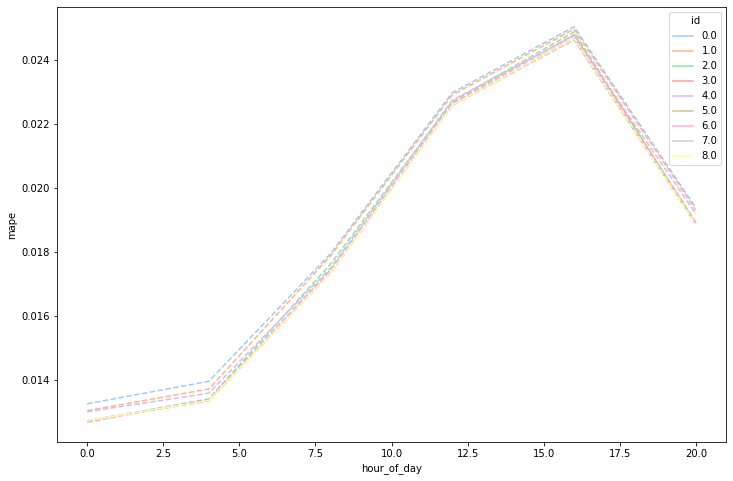
\includegraphics[width=1\linewidth,height=0.3\textheight]{images/MAPEtuning} \caption{MAPE for each SARIMA model}\label{fig:MAPEsarima}
\end{figure}

\subsection{Model Construction}\label{model-construction-1}

\textbf{SARIMA - Model 1}

\bigskip

The first model used only lagged versions of the forecast error for predicting the forecast error (Equation \eqref{eq:sarima1}).

\begin{equation}
\varepsilon^{\text{(SARIMA1)}}_{t} = \text{SARIMA}(6,0,2)(1,0,1,7)
\label{eq:sarima1}
\end{equation}\\
\noindent \textbf{SARIMA - Model 2}

\bigskip

The second model used lagged versions of the forecast error and exogenous data (forecast temperature, humidity, wind and rainfall) for predicting the forecast error (Equation \eqref{eq:sarima2}).

\begin{equation}
\begin{split}
\varepsilon^{\text(SARIMA2)}_t =& \text(SARIMA)(6,0,2)(1,0,1,7) + \\
& \theta_{1}forecastTemperature_t + \\
& \theta_{2}forecastHumidity_t + \theta_{3}forecastWind_t + \\
& \theta_{4}forecastRain_t
\end{split}
\label{eq:sarima2}
\end{equation}

\subsection{Model Performance}\label{model-performance-1}

The predicted forecast error was then used to update the forecast error (Equation \eqref{eq:oneC}). Model evaluation (MSE and MAPE) can be seen below.

\begin{multicols}{3}
\noindent\textbf{Old Model}\\
\textbf{Performance}\\
- MSE: 55078.33198 \\
- MAPE: 2.178\% \\


\columnbreak


\noindent\textbf{SARIMA Model} \\
\textbf{(no Exog) Performance} \\
- MSE: 49519.31974\\
- MAPE: 2.049\%\\

\columnbreak


\noindent\textbf{SARIMA Model (with} \\ 
\textbf{Exog) Performance} \\
- MSE: 49165.32932 \\
- MAPE: 2.082\% \\
\end{multicols}

Model 1 performed better as it minimised MAPE, which was given greater importance.

\section{Random Forest}\label{random-forest}

Random Forest is an ensemble learning method that operates by constructing multiple decision trees during training and outputting the average prediction of the individual trees.

The Random Forest model discussed aims to reduce the demand forecast error by predicting demand directly rather than predicting the error and then updating the original forecast.

\subsection{Model Construction}\label{model-construction-2}

\textbf{RFMF1 - Model 1}\\
The first model used the lag of the forecast error. The accuracy of predictions improved slightly in this model.
\bigskip

\noindent\textbf{RFMF1 - Model 2}\\
The second model used the lag of the forecast error and included weather variables (forecast temperature, wind speed, humidity and rain). The model predictions improved in this model (Figure \ref{fig:ForestModel2}).

\subsection{Parameter Selection (Fine Tuning)}\label{parameter-selection-fine-tuning}

Fine tuning was done by utilising Grid Search on the Random Forest Model.

\bigskip

By trialing many parameters combinations, the following combination was found to be the best performing.

\begin{align*}
n\_estimators&=200\\ 
max\_depth&=10\\ 
min\_samples\_split&=5\\ 
min\_samples\_leaf&=2\\
\end{align*}

\noindent Where \(n\_estimator\) is the number of trees, \(max\_depth\) is the maximum depth of each individual tree, \(min\_samples\_split\) is the minimum number of samples required to split an internal node and, \(min\_samples\_leaf\) is the minimum number of samples required to be at a leaf node.

\subsection{Model Performance}\label{model-performance-2}

Setting up models with the values above had the following results (Figure \ref{fig:ForestModel1}, Figure \ref{fig:ForestModel2}):

\begin{multicols}{2}
\noindent\textbf{RFMF1 Performance} \\
- MSE: 51971.086 \\
- MAPE: 2.111% \\


\columnbreak


\noindent\textbf{RFMF2 Performance} \\
- MSE: 51395.334\\
- MAPE: 2.095%\\
\end{multicols}

\begin{figure}
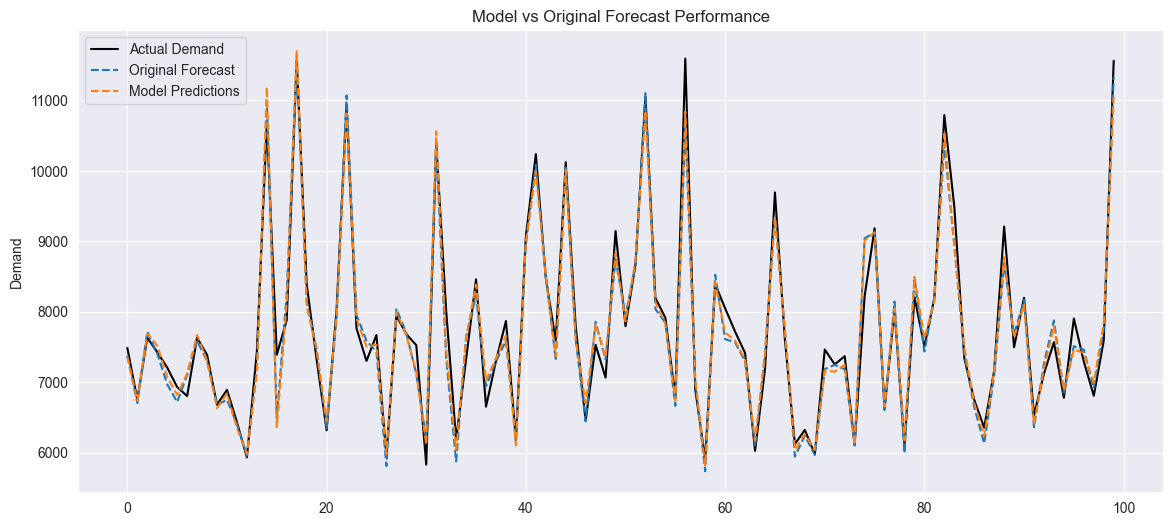
\includegraphics[width=1\linewidth,height=0.3\textheight]{images/ForestModel1} \caption{Line Plot of RFMF1's Performance vs Original Forecast Model Performance}\label{fig:ForestModel1}
\end{figure}

\begin{figure}
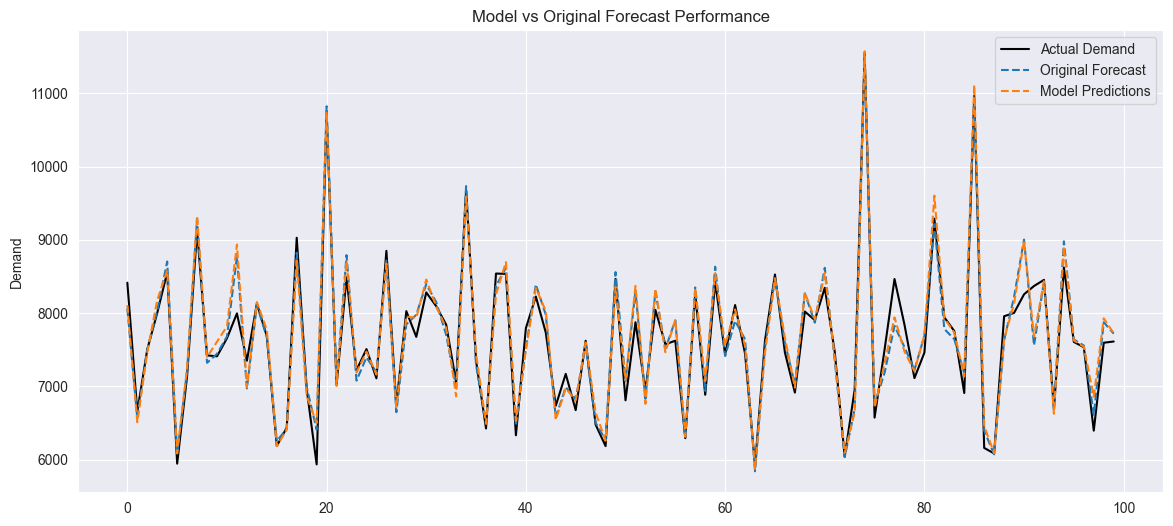
\includegraphics[width=1\linewidth,height=0.3\textheight]{images/ForestModel2} \caption{Line Plot of RFMF2's Performance vs Original Forecast Model Performance}\label{fig:ForestModel2}
\end{figure}

\section{XGBoost}\label{xgboost}

Extreme Gradient Boosting (XGBoost) is a machine learning algorithm that utilises gradient boosting decision trees that generates fast and effective models used for forecasting, classification and regression problems.

\bigskip

As discussed above, forecasting has been seen to improve when incorporating the new weather forecast values combined with previous errors. The overall aim being to reduce the demand forecast error.

\bigskip

The XGBoost model discussed aims to reduce the demand forecast error by predicting demand directly rather than predicting the error and then updating the original forecast.

\subsection{Model Construction}\label{model-construction-3}

The base model involved using forecasted temperature, humidity, wind speed and rain, combining that with the hour, month and the day of week. Taking the model to the next level involved including the previous forecasted demand and the previous forecast error from 24 hours, 48 hours, 7 days and 14 days ago.

\bigskip

Assessing where a base model performs worse based on hour of day yields the following.

\bigskip

\begin{figure}
\includegraphics[width=1\linewidth,height=0.3\textheight]{images/MAPEXGBoost} \caption{MAPE by Hour of the Day}\label{fig:MAPEXGBoost}
\end{figure}

\bigskip

Taking this error as a wave format, the model improved when variables were combined with a sin or cos wave. Specifically, combining hour with sin/cos wave and then multiplying by forecasted temperature improved the model.

\subsection{Parameter Selection (Fine Tuning)}\label{parameter-selection-fine-tuning-1}

Fine tuning is especially important for XGBoost and a grid search was utilised to find the highest performing combination from a wide distribution of parameters. The following was found to be the most effective combination of parameters.

\begin{center}
\begin{align*}
learning\_rate &= 0.1,\\
n\_estimators &= 150,\\
max\_depth &= 3,\\
subsample &= 0.8
\end{align*}
\end{center}

\subsection{Model Performance}\label{model-performance-3}

Utilising the above parameters gave accuracy scores of

\begin{align*}
\text{MSE} &= 46526.86 \\
\text{MAPE} &= 2.042\%
\end{align*}

\subsection{Combining variables}\label{combining-variables}

Introducing new variables as functions of other variables boosted the performance of XGBoost. Whilst in theory introducing variables such as Temperature * Humidity could improve the model, introducing them created unnecessary complexity that reduced the accuracy of the model. It could also been seen that XGBoost took these into account inside the algorithm.

\section{Model Comparison}\label{model-comparison}

Comparison of all models tested against the baseline AEMO model (Table \ref{tab:tab8}). The XG Boost model produced the highest level of accuracy of the models considered. This is further evident when observing prediction error distribution (Figure \ref{fig:Cpmparison}).

\begin{table}[H]
\caption{Models compared by MSE and MAPE}
\centering
\begin{tabular}{|ll|cc|}
\hline
\multicolumn{2}{|l|}{\multirow{2}{*}{}} & \multicolumn{2}{c|}{\textbf{Measure}} \\ \cline{3-4} 
\multicolumn{2}{|l|}{} & \multicolumn{1}{c|}{MSE} & MAPE \\ \hline
\multicolumn{1}{|l|}{\multirow{5}{*}{\textbf{Model}}} & {\textbf{AEMO}} & \multicolumn{1}{c|}{{55,159}} & {2.190\%} \\ \cline{2-4} 
\multicolumn{1}{|l|}{} & \textbf{Linear Regression} & \multicolumn{1}{c|}{49,718} & 2.080\% \\ \cline{2-4} 
\multicolumn{1}{|l|}{} & \textbf{SARIMA} & \multicolumn{1}{c|}{49,519} & 2.049\% \\ \cline{2-4} 
\multicolumn{1}{|l|}{} & \textbf{XGBoost} & \multicolumn{1}{c|}{46,526} & 2.042\% \\ \cline{2-4} 
\multicolumn{1}{|l|}{} & \textbf{Random Forest} & \multicolumn{1}{c|}{51,395} & 2.095\% \\ \hline
\end{tabular}
\label{tab:tab8}
\end{table}

\begin{figure}
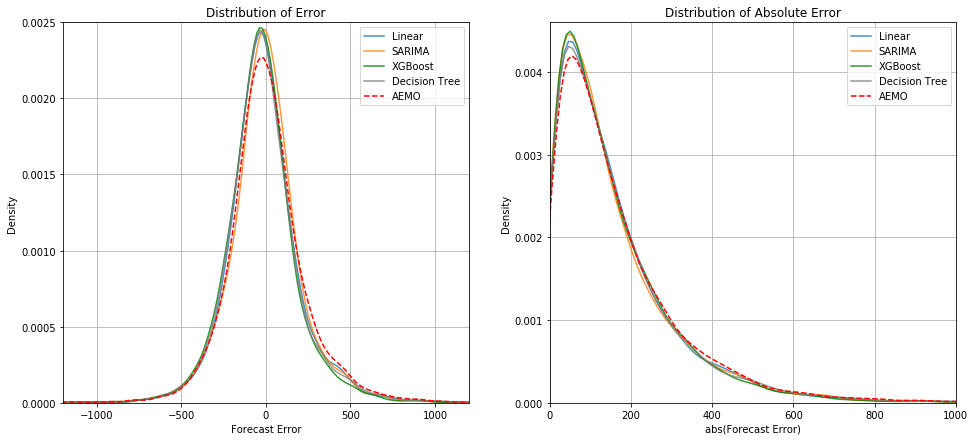
\includegraphics[width=1\linewidth,height=0.3\textheight]{images/Comparison} \caption{MSE Distribution}\label{fig:Cpmparison}
\end{figure}

\section{Summary of Key Findings}\label{summary-of-key-findings-1}

\begin{itemize}
\item
  \textbf{All models outperformed AEMO's model in terms of MSE and MAPE.} This indicates that there are likely underlying patterns in the AEMO residuals that are not currently captured in their model, therefore their model could be improved. This also validates forecasting methodologies which aims to use forecasting errors in modelling to further improve forecasting accuracy.
\item
  \textbf{XGBoost performed best compared with linear regression, SARIMA and Decision trees.} This may indicate that some underlying patterns in AEMO's forecast errors are likely non-linear, and therefore best forecasted by a black box method that can handle non-linear relationships.
\item
  \textbf{SARIMA also performed strongly}, indicating seasonality in the forecast error. This reinforces EDA findings where correlations existed between lagged forecast errors and current forecast errors. The SARIMA model also performed quite strongly based on MSE and MAPE. Furthermore, the SARIMA model which only included the lagged error performed the strongest, which provides further evidence of this relationship.
\item
  \textbf{Both machine learning models performed better when including weather related variables.} This may indicate a non-linear relationship between the forecast error (at least partly) and weather indicators (note, SARIMA would be limited in its ability to capture non-linearity).
\end{itemize}

\newpage

\chapter{Discussion}\label{discussion}

\section{Interpretation of results}\label{interpretation-of-results}

The results of this project demonstrate the validity of using forecast errors in modelling to further improve electricity demand predictions. This is particularly important for short-term energy demand forecasting which relies on the precision of forecasts to balance electricity demand and supply rather than requiring an interpretable model.

\bigskip

While XGBoost was the best performing model for the datasets considered, this may not be the case for all forecasts, depending on the underlying patterns in the forecast errors. If patterns in forecast errors are linear, traditional models such as ARIMA may perform better to improve the forecast. On the other hand, this project demonstrated that non-linear trends were present in the forecast errors which allowed the XGBoost model to be the better performing model.

\bigskip

Both machine learning methods performed better when incorporating weather indicator variables which may point to different models capturing different types of relationships (e.g.~SARIMA capturing the effect of the lagged error and XGBoost capturing effects of weather-related variables). This could indicate that modelling the forecast errors of the best model (XGBoost) with a different model (e.g.~SARIMA) has the potential to produce even more accurate results.

\section{Implications for energy planning}\label{implications-for-energy-planning}

Future short-term electricity forecasts should consider how residuals could be used to further improve forecasting accuracy. This could involve decomposing the data in the first instance as others have done and discussed in the literature review, or incorporating residuals from an initial forecasted model in a subsequent model. Improving forecast accuracy will likely have the benefit of greater efficiency in managing electricity generation.

\bigskip

It should be noted that the method described in this report has proven useful to increase accuracy of forecast predictions which is essential for short-term forecasting, however may not be appropriate for longer-term forecasting where interpretability of the model is more important.

\section{Limitations, challenges, and further research}\label{limitations-challenges-and-further-research}

While this project was able to improve on the AEMO forecast by modelling the forecast error, there is the potential that this could have been achieved more efficiently if a detailed AEMO forecasting methodology was available. This could have provided a better idea of what information or trends could be missing from the original forecast, and therefore which method would have been most useful to model the residuals.

\bigskip

This study only considered 12-hour interval due to the complexity of including several intervals and computational burden. Future research could consider longer or shorter forecast intervals to test the impact of modelling forecasting errors to improve accuracy for different intervals. Further research could also consider forecasting model errors using multiple models to capture the different patterns of errors.

\chapter{Conclusion and Further Issues}\label{conclusion-and-further-issues}

Hybrid models are known to improve the accuracy of electricity demand forecasts. This report took the concepts of a hybrid model to improve AEMO's short-term electricity demand forecast by incorporating AEMO forecast errors in a subsequent model to produce a more accurate prediction. The report found that for all models tested, the accuracy of the short-term forecast improved. This is valuable to industry as balancing the supply and demand of energy requires highly accurate forecasting. While this report only considered a 12-hour forecast interval, future studies could investigate different forecast intervals or multiple-iteration error-corrections to improve the accuracy of energy demand forecasts.

\newpage

\chapter*{References}\label{references}
\addcontentsline{toc}{chapter}{References}

\begin{hangparas}{.25in}{1}
Abbasi, R.A., Javaid, N., Ghuman, M.N.J., Khan, Z.A., Ur Rehman, S. \& Amanullah (2019). ‘Short Term Load Forecasting Using XGBoost’, \textit{Advances in Intelligent Systems and Computing}, pp.1120–1131. doi:\url{https://doi.org/10.1007/978-3-030-15035-8_108}.

AEMO. (2023). Load forecasting. Available at: \url{https://aemo.com.au/-/media/files/electricity/nem/security_and_reliability/power_system_ops/procedures/so_op_3710-load-forecasting.pdf?la=en} [Accessed 24 Mar. 2025].

Ahmad, A.S., Hassan, M.Y., Abdullah, M.P., Rahman, H.A., Hussin, F., Abdullah, H. \& Saidur, R. (2014). ‘A review on applications of ANN and SVM for building electrical energy consumption forecasting’, \textit{Renewable and Sustainable Energy Reviews}, [online] 33, pp.102–109. doi:\url{https://doi.org/10.1016/j.rser.2014.01.069}.

Ahmad, T. \& Chen, H. (2018). ‘Potential of three variant machine-learning models for forecasting district level medium-term and long-term energy demand in smart grid environment’, \textit{Energy}, 160, pp.1008–1020. doi:\url{https://doi.org/10.1016/j.energy.2018.07.084}.

Ahmad, W., Ayub, N., Ali, T., Irfan, M., Awais, M., Shiraz, M. \& Glowacz, A. (2020). ‘Towards short term electricity load forecasting using improved support vector machine and extreme learning machine’, \textit{Energies}, 13(11), p.2907. doi:\url{https://doi.org/10.3390/en13112907}.

Amara, F., Agbossou, K., Dubé, Y., Kelouwani, S., Cardenas, A. \& Hosseini, S.S. (2019). ‘A residual load modeling approach for household short-term load forecasting application’, \textit{Energy and Buildings}, 187, pp.132–143. doi:\url{https://doi.org/10.1016/j.enbuild.2019.01.009}.

Andronikos, A., Tzelepi, M. \& Tefas, A. (2023). ‘Residual Error Learning for Electricity Demand Forecasting’, In: Iliadis, L., Maglogiannis, I., Alonso, S., Jayne, C. \& Pimenidis, E. (eds) \textit{Engineering Applications of Neural Networks}. EANN 2023. Communications in Computer and Information Science, vol 1826. Springer, Cham. doi:\url{https://doi.org/10.1007/978-3-031-34204-2_33}.

Añel, J.A., Pérez-Souto, C., Bayo-Besteiro, S., Prieto-Godino, L., Bloomfield, H., Troccoli, A. \& Laura (2024). ‘Extreme weather events and the energy sector in 2021’, \textit{Weather Climate and Society}. doi:\url{https://doi.org/10.1175/wcas-d-23-0115.1}.

Ardakani, F.J. \& Ardehali, M.M. (2014). ‘Long-term electrical energy consumption forecasting for developing and developed economies based on different optimized models and historical data types’, \textit{Energy}, 65, pp.452–461. doi:\url{https://doi.org/10.1016/j.energy.2013.12.031}.

Boroojeni, K.G., Amini, M.H., Bahrami, S., Iyengar, S.S., Sarwat, A.I. \& Karabasoglu, O. (2017). ‘A novel multi-time-scale modeling for electric power demand forecasting: From short-term to medium-term horizon’, \textit{Electric Power Systems Research}, 142, pp.58–73. doi:\url{https://doi.org/10.1016/j.epsr.2016.08.031}.

Deng, X., Ye, A., Zhong, J., Xu, D., Yang, W., Song, Z., Zhang, Z., Guo, J., Wang, T., Tian, Y., Pan, H., Zhang, Z., Wang, H., Wu, C., Shao, J. \& Chen, X. (2022). ‘Bagging–XGBoost algorithm based extreme weather identification and short-term load forecasting model’, \textit{Energy Reports}, 8, pp.8661–8674. doi:\url{https://doi.org/10.1016/j.egyr.2022.06.072}.

Divina, F., García Torres, M., Goméz Vela, F.A. \& Vázquez Noguera, J.L. (2019). ‘A Comparative Study of Time Series Forecasting Methods for Short Term Electric Energy Consumption Prediction in Smart Buildings’, \textit{Energies}, 12(10), p.1934. doi:\url{https://doi.org/10.3390/en12101934}.

Ediger, V.Ş. \& Akar, S. (2007). ‘ARIMA forecasting of primary energy demand by fuel in Turkey’, \textit{Energy Policy}, 35(3), pp.1701–1708. doi: \url{https://doi.org/10.1016/j.enpol.2006.05.009}.

Ertuğrul, Ö.F., Tekin, H. \& Tekin, R. (2020). ‘A novel regression method in forecasting short-term grid electricity load in buildings that were connected to the smart grid’, \textit{Electrical Engineering}, 103, pp: 717-728.  doi:\url{https://doi.org/10.1007/s00202-020-01114-3}.

Ghalehkhondabi, I., Ardjmand, E., Weckman, G.R. \& Young, W.A. (2016). ‘An overview of energy demand forecasting methods published in 2005–2015’, \textit{Energy Systems}, 8(2), pp.411–447. doi:\url{https://doi.org/10.1007/s12667-016-0203-y}.

Klyuev, R.V., Morgoev, I.D., Morgoeva, A.D., Gavrina, O.A., Martyushev, N.V., Efremenkov, E.A. \& Mengxu, Q. (2022). ‘Methods of Forecasting Electric Energy Consumption: A Literature Review’, \textit{Energies}, 15(23), p.8919. doi:\url{https://doi.org/10.3390/en15238919}.

Kopyt, M., Piotrowski, P. \& Baczyński, D. (2024). ‘Short-Term Energy Generation Forecasts at a Wind Farm—A Multi-Variant Comparison of the Effectiveness and Performance of Various Gradient-Boosted Decision Tree Models’, \textit{Energies}, 17(23), p.6194. doi:\url{https://doi.org/10.3390/en17236194}.

Koukaras, P., Mustapha, A., Mystakidis, A. \& Tjortjis, C. (2024). ‘Optimizing Building Short-Term Load Forecasting: A Comparative Analysis of Machine Learning Models’, \textit{Energies}, 17(6), p.1450. doi:\url{https://doi.org/10.3390/en17061450}.

Kuo, P.-H. \& Huang, C.-J. (2018). ‘A High Precision Artificial Neural Networks Model for Short-Term Energy Load Forecasting’, \textit{Energies}, 11(1), p.213. doi:\url{https://doi.org/10.3390/en11010213}.

Liu, X.-Q., Zhang, C., Zhou, Y. \& Liao, H. (2021). ‘Temperature change and electricity consumption of the group living: A case study of college students’, \textit{Science of The Total Environment}, 781, p.146574. doi:\url{https://doi.org/10.1016/j.scitotenv.2021.146574}.

Maia-Silva, D., Kumar, R. \& Nateghi, R. (2020). ‘The critical role of humidity in modeling summer electricity demand across the United States’, \textit{Nature Communications}, 11, p.1686. doi:\url{https://doi.org/10.1038/s41467-020-15393-8}.

Manno, A., Martelli, E. and Amaldi, E. (2022). ‘A Shallow Neural Network Approach for the Short-Term Forecast of Hourly Energy Consumption’, \textit{Energies}, [online] 15(3), pp.958. doi:\url{https://doi.org/10.3390/en15030958}. 

Marco G. Pinheiro, Sara C. Madeira, Alexandre P. Francisco, (2023). ‘Short-term electricity load forecasting—A systematic approach from system level to secondary substations’, \textit{Applied Energy}, 332, pp.120493, ISSN 0306-2619, doi:\url{https://doi.org/10.1016/j.apenergy.2022.120493}.  

Mystakidis, A., Koukaras, P., Tsalikidis, N., Ioannidis, D. and Tjortjis, C. (2024). ‘Energy Forecasting: A Comprehensive Review of Techniques and Technologies’, \textit{Energies}, [online] 17(7), pp.1662. doi:\url{https://doi.org/10.3390/en17071662}.  

OpenWeather. (2025). \textit{Custom Weather Products.} [Online] Available at: \url{https://home.openweathermap.org/marketplace} [Accessed 29 Mar. 2025] 

Pao, H.T. (2009). Forecasting energy consumption in Taiwan using hybrid nonlinear models. \textit{Energy}, 34(10), pp.1438–1446. doi:\url{https://doi.org/10.1016/j.energy.2009.04.026}. 

Papalexopoulos, A.D. and Hesterberg, T.C. (1990). ‘A regression-based approach to short-term system load forecasting’, \textit{IEEE Transactions on Power Systems}, 5(4), pp.1535–1547. doi:\url{https://doi.org/10.1109/59.99410}.  

Phyo, P.P. and Byun, Y.-C. (2021). ‘Hybrid Ensemble Deep Learning-Based Approach for Time Series Energy Prediction’, \textit{Symmetry}, 13(10), pp.1942. doi:\url{https://doi.org/10.3390/sym13101942}.  

Rakpho, P. and Yamaka, W. (2021). ‘The forecasting power of economic policy uncertainty for energy demand and supply’, \textit{Energy Reports}, 7, pp.338–343. doi:\url{https://doi.org/10.1016/j.egyr.2021.06.059}.   

Sanhudo, L., Rodrigues, J. and Filho, Ê.V. (2021). ‘Multivariate time series clustering and forecasting for building energy analysis: Application to weather data quality control’, \textit{Journal of Building Engineering}, 35, pp.101996. doi:\url{https://doi.org/10.1016/j.jobe.2020.101996}.  

Savić, S., Selakov, A. and Milošević, D. (2014). ‘Cold and warm air temperature spells during the winter and summer seasons and their impact on energy consumption in urban areas’, \textit{Natural Hazards}, 73(2), pp.373–387. doi:\url{https://doi.org/10.1007/s11069-014-1074-y}.  

Singh, S. and Yassine, A. (2018). ‘Big Data Mining of Energy Time Series for Behavioral Analytics and Energy Consumption Forecasting’, \textit{Energies}, 11(2), pp.452. doi:\url{https://doi.org/10.3390/en11020452}.  

Suganthi, L. and Samuel, A.A. (2012). ‘Energy models for demand forecasting—A review’, \textit{Renewable and Sustainable Energy Reviews}, 16(2), pp.1223–1240. doi:\url{https://doi.org/10.1016/j.rser.2011.08.014}.    

Tarmanini, C., Sarma, N., Gezegin, C. and Ozgonenel, O. (2023). ‘Short term load forecasting based on ARIMA and ANN approaches’, \textit{Energy Reports}, 9, pp.550–557. doi:\url{https://doi.org/10.1016/j.egyr.2023.01.060}.  

Wang, J., Li, P., Ran, R., Che, Y. and Zhou, Y. (2018). ‘A Short-Term Photovoltaic Power Prediction Model Based on the Gradient Boost Decision Tree’, \textit{Applied Sciences}, 8(5), pp.689. doi:\url{https://doi.org/10.3390/app8050689}. 

Zhang, S., Guo, Q., Smyth, R. and Yao, Y. (2022). ‘Extreme temperatures and residential electricity consumption: Evidence from Chinese households’, \textit{Energy Economics}, pp.105890. doi:\url{https://doi.org/10.1016/j.eneco.2022.105890}.  
\end{hangparas}

\newpage

\chapter*{Appendix}\label{appendix}
\addcontentsline{toc}{chapter}{Appendix}

\appendix

\section*{Appendix A: Data Processing}\label{appendix-a-data-processing}
\addcontentsline{toc}{section}{Appendix A: Data Processing}

Packages used for data cleaning

\begin{Shaded}
\begin{Highlighting}[]
\ImportTok{import}\NormalTok{ pandas }\ImportTok{as}\NormalTok{ pd}
\ImportTok{import}\NormalTok{ numpy }\ImportTok{as}\NormalTok{ np}

\NormalTok{pd.options.mode.chained\_assignment }\OperatorTok{=} \VariableTok{None}
\end{Highlighting}
\end{Shaded}

Importing the data

\begin{Shaded}
\begin{Highlighting}[]
\CommentTok{\# Forecast Data}
\CommentTok{\#\# Reading data and formating data{-}time columns}
\NormalTok{df\_forecast }\OperatorTok{=}\NormalTok{ pd.read\_csv(}\StringTok{\textquotesingle{}data/forecastdemand\_nsw.csv\textquotesingle{}}\NormalTok{, names }\OperatorTok{=} 
\NormalTok{    [}\StringTok{\textquotesingle{}id\textquotesingle{}}\NormalTok{, }\StringTok{\textquotesingle{}region\_id\textquotesingle{}}\NormalTok{, }\StringTok{\textquotesingle{}period\_id\textquotesingle{}}\NormalTok{, }\StringTok{\textquotesingle{}forecast\_demand\textquotesingle{}}\NormalTok{, }
    \StringTok{\textquotesingle{}date\_time\_current\textquotesingle{}}\NormalTok{, }\StringTok{\textquotesingle{}date\_time\_future\textquotesingle{}}\NormalTok{], skiprows }\OperatorTok{=} \DecValTok{1}\NormalTok{)}
\NormalTok{df\_forecast.date\_time\_current }\OperatorTok{=}\NormalTok{ pd.to\_datetime(}
\NormalTok{    df\_forecast.date\_time\_current, }\BuiltInTok{format} \OperatorTok{=} \StringTok{"\%Y{-}\%m{-}}\SpecialCharTok{\%d}\StringTok{ \%H:\%M:\%S"}\NormalTok{)}
\NormalTok{df\_forecast.date\_time\_future }\OperatorTok{=}\NormalTok{ pd.to\_datetime(}
\NormalTok{    df\_forecast.date\_time\_future, }\BuiltInTok{format} \OperatorTok{=} \StringTok{"\%Y{-}\%m{-}}\SpecialCharTok{\%d}\StringTok{ \%H:\%M:\%S"}\NormalTok{)}

\CommentTok{\#\# Using \textquotesingle{}period\_id\textquotesingle{} to round \textquotesingle{}current time\textquotesingle{}}
\NormalTok{df\_forecast[}\StringTok{"date\_time\_current\_rounded"}\NormalTok{] }\OperatorTok{=}\NormalTok{ df\_forecast.period\_id.}\BuiltInTok{apply}\NormalTok{(}
    \KeywordTok{lambda}\NormalTok{ x: pd.Timedelta(hours }\OperatorTok{=}\NormalTok{ x}\OperatorTok{/}\DecValTok{2}\NormalTok{))}
\NormalTok{df\_forecast.date\_time\_current\_rounded }\OperatorTok{=}\NormalTok{ df\_forecast.date\_time\_future }\OperatorTok{{-}}
\NormalTok{    df\_forecast.date\_time\_current\_rounded}

\CommentTok{\# Demand Data}
\CommentTok{\#\# Reading data and formating data{-}time columns}
\NormalTok{df\_demand }\OperatorTok{=}\NormalTok{ pd.read\_csv(}\StringTok{\textquotesingle{}data/totaldemand\_nsw.csv\textquotesingle{}}\NormalTok{, names }\OperatorTok{=} 
\NormalTok{    [}\StringTok{\textquotesingle{}date\_time\textquotesingle{}}\NormalTok{, }\StringTok{\textquotesingle{}total\_demand\textquotesingle{}}\NormalTok{, }\StringTok{\textquotesingle{}region\_id\textquotesingle{}}\NormalTok{], skiprows }\OperatorTok{=} \DecValTok{1}\NormalTok{)}
\NormalTok{df\_demand.date\_time }\OperatorTok{=}\NormalTok{ pd.to\_datetime(df\_demand.date\_time, }
    \BuiltInTok{format} \OperatorTok{=} \StringTok{"}\SpecialCharTok{\%d}\StringTok{/\%m/\%Y \%H:\%M"}\NormalTok{)}


\CommentTok{\# Forecast temperature data}
\NormalTok{df\_weather\_forecast }\OperatorTok{=}\NormalTok{ pd.read\_csv(}\StringTok{\textquotesingle{}data/forecast\_temperatre.csv\textquotesingle{}}\NormalTok{)}

\NormalTok{df\_weather\_forecast }\OperatorTok{=}\NormalTok{ df\_weather\_forecast.rename(}
\NormalTok{  \{}\StringTok{\textquotesingle{}forecast dt iso\textquotesingle{}}\NormalTok{: }\StringTok{\textquotesingle{}date\_time\_current\_utc\textquotesingle{}}\NormalTok{, }
   \StringTok{\textquotesingle{}slice dt iso\textquotesingle{}}\NormalTok{: }\StringTok{\textquotesingle{}date\_time\_future\_utc\textquotesingle{}}\NormalTok{,}
   \StringTok{\textquotesingle{}temperature\textquotesingle{}}\NormalTok{: }\StringTok{\textquotesingle{}temperature\_future\_forecast\textquotesingle{}}\NormalTok{,}
   \StringTok{\textquotesingle{}humidity\textquotesingle{}}\NormalTok{: }\StringTok{\textquotesingle{}humidity\_future\_forecast\textquotesingle{}}\NormalTok{,}
   \StringTok{\textquotesingle{}rain\textquotesingle{}}\NormalTok{: }\StringTok{\textquotesingle{}rain\_future\_forecast\textquotesingle{}}\NormalTok{,}
   \StringTok{\textquotesingle{}wind\_speed\textquotesingle{}}\NormalTok{: }\StringTok{\textquotesingle{}wind\_speed\_future\_forecast\textquotesingle{}}\NormalTok{\}, axis }\OperatorTok{=} \DecValTok{1}\NormalTok{)}

\NormalTok{df\_weather\_forecast[}\StringTok{"date\_time\_current\_rounded"}\NormalTok{] }\OperatorTok{=}   
\NormalTok{    pd.to\_datetime(df\_weather\_forecast.date\_time\_current\_utc, }
    \BuiltInTok{format} \OperatorTok{=} \StringTok{"\%Y{-}\%m{-}}\SpecialCharTok{\%d}\StringTok{ \%H:\%M:\%S +0000 UTC"}\NormalTok{) }\OperatorTok{+}\NormalTok{ pd.Timedelta(hours }\OperatorTok{=} \DecValTok{10}\NormalTok{)}
\NormalTok{df\_weather\_forecast[}\StringTok{"date\_time\_future"}\NormalTok{] }\OperatorTok{=} 
\NormalTok{    pd.to\_datetime(df\_weather\_forecast.date\_time\_future\_utc, }
    \BuiltInTok{format} \OperatorTok{=} \StringTok{"\%Y{-}\%m{-}}\SpecialCharTok{\%d}\StringTok{ \%H:\%M:\%S +0000 UTC"}\NormalTok{) }\OperatorTok{+}\NormalTok{ pd.Timedelta(hours }\OperatorTok{=} \DecValTok{10}\NormalTok{)}

\NormalTok{df\_weather\_forecast }\OperatorTok{=} 
\NormalTok{    df\_weather\_forecast[[}\StringTok{\textquotesingle{}date\_time\_current\_rounded\textquotesingle{}}\NormalTok{, }\StringTok{\textquotesingle{}date\_time\_future\textquotesingle{}}\NormalTok{, }
      \StringTok{\textquotesingle{}temperature\_future\_forecast\textquotesingle{}}\NormalTok{, }\StringTok{\textquotesingle{}humidity\_future\_forecast\textquotesingle{}}\NormalTok{, }
      \StringTok{\textquotesingle{}rain\_future\_forecast\textquotesingle{}}\NormalTok{, }\StringTok{\textquotesingle{}wind\_speed\_future\_forecast\textquotesingle{}}\NormalTok{]]}
\end{Highlighting}
\end{Shaded}

Merging the data

\begin{Shaded}
\begin{Highlighting}[]
\CommentTok{\#Merging Datasets}
\NormalTok{df\_all }\OperatorTok{=}\NormalTok{ pd.merge(df\_forecast, df\_demand[[}\StringTok{"date\_time"}\NormalTok{, }\StringTok{"total\_demand"}\NormalTok{]], }
\NormalTok{    left\_on }\OperatorTok{=} \StringTok{"date\_time\_future"}\NormalTok{, right\_on }\OperatorTok{=} \StringTok{"date\_time"}\NormalTok{).drop(}
\NormalTok{        columns }\OperatorTok{=} \StringTok{"date\_time"}\NormalTok{)}

\NormalTok{df\_all }\OperatorTok{=}\NormalTok{ pd.merge(df\_all, }
\NormalTok{    df\_temperature[[}\StringTok{"date\_time\_30m"}\NormalTok{, }\StringTok{"temperature"}\NormalTok{]], }
\NormalTok{        left\_on }\OperatorTok{=} \StringTok{"date\_time\_future"}\NormalTok{, right\_on }\OperatorTok{=} \StringTok{"date\_time\_30m"}\NormalTok{)}
\NormalTok{df\_all }\OperatorTok{=}\NormalTok{ df\_all.drop(}
\NormalTok{    columns }\OperatorTok{=}\NormalTok{ [}\StringTok{"date\_time\_30m"}\NormalTok{, }\StringTok{"region\_id"}\NormalTok{]).rename(}
\NormalTok{        \{}\StringTok{"temperature"}\NormalTok{: }\StringTok{"temperature\_future"}\NormalTok{\}, axis }\OperatorTok{=} \DecValTok{1}\NormalTok{)}

\NormalTok{df\_all }\OperatorTok{=}\NormalTok{ pd.merge(df\_all, }
\NormalTok{    df\_temperature[[}\StringTok{"date\_time\_30m"}\NormalTok{, }\StringTok{"temperature"}\NormalTok{]], }
\NormalTok{    left\_on }\OperatorTok{=} \StringTok{"date\_time\_current\_rounded"}\NormalTok{, right\_on }\OperatorTok{=} \StringTok{"date\_time\_30m"}\NormalTok{)}
\NormalTok{df\_all }\OperatorTok{=}\NormalTok{ df\_all.drop(columns }\OperatorTok{=} 
    \StringTok{"date\_time\_30m"}\NormalTok{).rename(\{}\StringTok{"temperature"}\NormalTok{: }\StringTok{"temperature\_current"}\NormalTok{\}, }
\NormalTok{    axis }\OperatorTok{=} \DecValTok{1}\NormalTok{)}

\NormalTok{df\_all }\OperatorTok{=}\NormalTok{ pd.merge(df\_all, df\_weather\_forecast, on }\OperatorTok{=} 
\NormalTok{    [}\StringTok{"date\_time\_current\_rounded"}\NormalTok{, }\StringTok{"date\_time\_future"}\NormalTok{], how }\OperatorTok{=} \StringTok{\textquotesingle{}left\textquotesingle{}}\NormalTok{)}
\end{Highlighting}
\end{Shaded}

Format data.

\begin{Shaded}
\begin{Highlighting}[]
\NormalTok{df\_all[}\StringTok{"forecast\_interval"}\NormalTok{] }\OperatorTok{=}\NormalTok{ df\_all.date\_time\_future }\OperatorTok{{-}} 
\NormalTok{    df\_all.date\_time\_current\_rounded}
\NormalTok{df\_all[}\StringTok{"forecast\_error"}\NormalTok{] }\OperatorTok{=}\NormalTok{ df\_all.total\_demand }\OperatorTok{{-}} 
\NormalTok{    df\_all.forecast\_demand}
\NormalTok{df\_all[}\StringTok{"forecast\_error\_relative"}\NormalTok{] }\OperatorTok{=} 
\NormalTok{    df\_all.forecast\_error}\OperatorTok{/}\NormalTok{df\_all.total\_demand}

\NormalTok{df\_all[}\StringTok{"date\_time\_future\_month"}\NormalTok{] }\OperatorTok{=}\NormalTok{ df\_all.date\_time\_future.dt.month}
\NormalTok{df\_all[}\StringTok{"date\_time\_future\_year"}\NormalTok{] }\OperatorTok{=}\NormalTok{ df\_all.date\_time\_future.dt.year}
\NormalTok{df\_all[}\StringTok{"date\_time\_future\_weekday"}\NormalTok{] }\OperatorTok{=}\NormalTok{ df\_all.date\_time\_future.dt.dayofweek}
\NormalTok{df\_all[}\StringTok{"date\_time\_future\_hour"}\NormalTok{] }\OperatorTok{=}\NormalTok{ df\_all.date\_time\_future.dt.hour}

\NormalTok{df\_all[}\StringTok{"week\_day\_name"}\NormalTok{] }\OperatorTok{=}\NormalTok{ df\_all.date\_time\_future.dt.day\_name()}

\NormalTok{df\_all[}\StringTok{"isSaturday"}\NormalTok{] }\OperatorTok{=}\NormalTok{ df\_all.week\_day\_name.}\BuiltInTok{apply}\NormalTok{(}
    \KeywordTok{lambda}\NormalTok{ x: }\DecValTok{1} \ControlFlowTok{if}\NormalTok{ x }\OperatorTok{==} \StringTok{\textquotesingle{}Saturday\textquotesingle{}} \ControlFlowTok{else} \DecValTok{0}\NormalTok{)}
\NormalTok{df\_all[}\StringTok{"isSunday"}\NormalTok{] }\OperatorTok{=}\NormalTok{ df\_all.week\_day\_name.}\BuiltInTok{apply}\NormalTok{(}
    \KeywordTok{lambda}\NormalTok{ x: }\DecValTok{1} \ControlFlowTok{if}\NormalTok{ x }\OperatorTok{==} \StringTok{\textquotesingle{}Sunday\textquotesingle{}} \ControlFlowTok{else} \DecValTok{0}\NormalTok{)}

\NormalTok{df\_all[}\StringTok{"isDecember"}\NormalTok{] }\OperatorTok{=}\NormalTok{ df\_all.date\_time\_future\_month.}\BuiltInTok{apply}\NormalTok{(}
    \KeywordTok{lambda}\NormalTok{ x: }\DecValTok{1} \ControlFlowTok{if}\NormalTok{ x }\OperatorTok{==} \DecValTok{12} \ControlFlowTok{else} \DecValTok{0}\NormalTok{)}
\NormalTok{df\_all[}\StringTok{"isJanuary"}\NormalTok{] }\OperatorTok{=}\NormalTok{ df\_all.date\_time\_future\_month.}\BuiltInTok{apply}\NormalTok{(}
    \KeywordTok{lambda}\NormalTok{ x: }\DecValTok{1} \ControlFlowTok{if}\NormalTok{ x }\OperatorTok{==} \DecValTok{1} \ControlFlowTok{else} \DecValTok{0}\NormalTok{)}
\NormalTok{df\_all[}\StringTok{"isFebruary"}\NormalTok{] }\OperatorTok{=}\NormalTok{ df\_all.date\_time\_future\_month.}\BuiltInTok{apply}\NormalTok{(}
    \KeywordTok{lambda}\NormalTok{ x: }\DecValTok{1} \ControlFlowTok{if}\NormalTok{ x }\OperatorTok{==} \DecValTok{2} \ControlFlowTok{else} \DecValTok{0}\NormalTok{)}
\NormalTok{df\_all[}\StringTok{"isNovember"}\NormalTok{] }\OperatorTok{=}\NormalTok{ df\_all.date\_time\_future\_month.}\BuiltInTok{apply}\NormalTok{(}
    \KeywordTok{lambda}\NormalTok{ x: }\DecValTok{1} \ControlFlowTok{if}\NormalTok{ x }\OperatorTok{==} \DecValTok{11} \ControlFlowTok{else} \DecValTok{0}\NormalTok{)}
\end{Highlighting}
\end{Shaded}

\newpage

\section*{Appendix B: Models}\label{appendix-b-models}
\addcontentsline{toc}{section}{Appendix B: Models}

\subsection*{B1. AEMO Model}\label{b1.-aemo-model}

Import packages

\begin{Shaded}
\begin{Highlighting}[]
\ImportTok{import}\NormalTok{ pandas }\ImportTok{as}\NormalTok{ pd}
\ImportTok{import}\NormalTok{ matplotlib.pyplot }\ImportTok{as}\NormalTok{ plt}
\ImportTok{import}\NormalTok{ numpy }\ImportTok{as}\NormalTok{ np}
\ImportTok{import}\NormalTok{ seaborn }\ImportTok{as}\NormalTok{ sns}
\ImportTok{import}\NormalTok{ statsmodels.api }\ImportTok{as}\NormalTok{ sm}

\ImportTok{from}\NormalTok{ sklearn.metrics }\ImportTok{import}\NormalTok{ mean\_squared\_error}
\ImportTok{from}\NormalTok{ sklearn.metrics }\ImportTok{import}\NormalTok{ mean\_absolute\_percentage\_error}
\ImportTok{from}\NormalTok{ matplotlib.pyplot }\ImportTok{import}\NormalTok{ figure}
\end{Highlighting}
\end{Shaded}

\begin{Shaded}
\begin{Highlighting}[]
\NormalTok{delta }\OperatorTok{=} \DecValTok{24}

\NormalTok{df\_lag }\OperatorTok{=}\NormalTok{ df\_all.loc[df\_all.period\_id }\OperatorTok{==}\NormalTok{ delta].sort\_values(}
    \StringTok{"date\_time\_future"}\NormalTok{).reset\_index(drop }\OperatorTok{=} \VariableTok{True}\NormalTok{)}
\NormalTok{df\_lag\_temp }\OperatorTok{=} 
\NormalTok{df\_lag.copy()[}
\NormalTok{  [}\StringTok{"forecast\_error"}\NormalTok{, }\StringTok{"forecast\_error\_relative"}\NormalTok{, }\StringTok{"date\_time\_future"}\NormalTok{]}
\NormalTok{  ].rename(\{}\StringTok{"forecast\_error"}\NormalTok{ : }\StringTok{"forecast\_error\_24h\_ago"}\NormalTok{, }
            \StringTok{"forecast\_error\_relative"}\NormalTok{: }\StringTok{"forecast\_error\_relative\_24h\_ago"}\NormalTok{,}
            \StringTok{"date\_time\_future"}\NormalTok{: }\StringTok{"date\_time\_future\_24h\_ago"}\NormalTok{\}, axis }\OperatorTok{=} \DecValTok{1}\NormalTok{)}
\NormalTok{df\_lag[}\StringTok{"date\_time\_current\_24h\_ago"}\NormalTok{] }\OperatorTok{=} 
\NormalTok{    df\_lag.date\_time\_current }\OperatorTok{{-}}\NormalTok{ pd.DateOffset(hours }\OperatorTok{=} \DecValTok{24}\NormalTok{)}
\NormalTok{df\_lag[}\StringTok{"date\_time\_future\_24h\_ago"}\NormalTok{] }\OperatorTok{=} 
\NormalTok{    df\_lag.date\_time\_future }\OperatorTok{{-}}\NormalTok{ pd.DateOffset(hours }\OperatorTok{=} \DecValTok{24}\NormalTok{)}

\NormalTok{df\_lag }\OperatorTok{=}\NormalTok{ df\_lag.loc[}
\NormalTok{      df\_lag.date\_time\_future\_24h\_ago }\OperatorTok{\textgreater{}=} \BuiltInTok{min}\NormalTok{(df\_lag.date\_time\_future)]}
\NormalTok{df\_lag }\OperatorTok{=}\NormalTok{ pd.merge(df\_lag, df\_lag\_temp, }
\NormalTok{    on }\OperatorTok{=} \StringTok{"date\_time\_future\_24h\_ago"}\NormalTok{, how }\OperatorTok{=} \StringTok{\textquotesingle{}left\textquotesingle{}}\NormalTok{)}
\NormalTok{df\_lag }\OperatorTok{=}\NormalTok{ df\_lag.loc[df\_lag.forecast\_error\_relative\_24h\_ago.notna()]}

\NormalTok{train\_test\_split }\OperatorTok{=} \FloatTok{0.7}
\NormalTok{split\_int }\OperatorTok{=} \BuiltInTok{int}\NormalTok{(train\_test\_split }\OperatorTok{*} \BuiltInTok{len}\NormalTok{(df\_lag))}
\NormalTok{df\_lag\_train, df\_lag\_test }\OperatorTok{=}\NormalTok{ df\_lag[:split\_int], df\_lag[split\_int:]}
\end{Highlighting}
\end{Shaded}

\begin{Shaded}
\begin{Highlighting}[]
\NormalTok{mse }\OperatorTok{=}\NormalTok{ mean\_squared\_error(df\_lag\_test.forecast\_demand, }
\NormalTok{    df\_lag\_test.total\_demand)}
\NormalTok{mape }\OperatorTok{=}\NormalTok{  mean\_absolute\_percentage\_error(df\_lag\_test.forecast\_demand, }
\NormalTok{    df\_lag\_test.total\_demand)}

\BuiltInTok{print}\NormalTok{(}\SpecialStringTok{f"Existing model MSE = }\SpecialCharTok{\{}\BuiltInTok{round}\NormalTok{(mse)}\SpecialCharTok{\}}\SpecialStringTok{"}\NormalTok{)}
\BuiltInTok{print}\NormalTok{(}\SpecialStringTok{f"Existing model MAPE = }\SpecialCharTok{\{}\BuiltInTok{round}\NormalTok{(}\DecValTok{100}\OperatorTok{*}\NormalTok{mape,}\DecValTok{2}\NormalTok{)}\SpecialCharTok{\}}\SpecialStringTok{\%"}\NormalTok{)}
\end{Highlighting}
\end{Shaded}

\subsection*{B2. Linear Regression}\label{b2.-linear-regression}

Import packages

\begin{Shaded}
\begin{Highlighting}[]
\ImportTok{import}\NormalTok{ pandas }\ImportTok{as}\NormalTok{ pd}
\ImportTok{import}\NormalTok{ matplotlib.pyplot }\ImportTok{as}\NormalTok{ plt}
\ImportTok{import}\NormalTok{ numpy }\ImportTok{as}\NormalTok{ np}
\ImportTok{import}\NormalTok{ seaborn }\ImportTok{as}\NormalTok{ sns}
\ImportTok{import}\NormalTok{ statsmodels.api }\ImportTok{as}\NormalTok{ sm}
\ImportTok{import}\NormalTok{ warnings}

\ImportTok{from}\NormalTok{ statsmodels.graphics.tsaplots }\ImportTok{import}\NormalTok{ plot\_acf, plot\_pacf}
\ImportTok{from}\NormalTok{ sklearn.metrics }\ImportTok{import}\NormalTok{ mean\_squared\_error}
\ImportTok{from}\NormalTok{ sklearn.metrics }\ImportTok{import}\NormalTok{ mean\_absolute\_percentage\_error}
\ImportTok{from}\NormalTok{ statsmodels.tsa.stattools }\ImportTok{import}\NormalTok{ adfuller}
\ImportTok{from}\NormalTok{ matplotlib.pyplot }\ImportTok{import}\NormalTok{ figure}
\ImportTok{from}\NormalTok{ statsmodels.graphics.api }\ImportTok{import}\NormalTok{ qqplot}
\end{Highlighting}
\end{Shaded}

\textbf{Linear Regression Model 1}

\begin{Shaded}
\begin{Highlighting}[]
\NormalTok{x\_columns }\OperatorTok{=}\NormalTok{ [}\StringTok{"forecast\_error\_24h\_ago"}\NormalTok{]}
\NormalTok{x }\OperatorTok{=}\NormalTok{ sm.add\_constant(df\_lag\_train[x\_columns])}
\NormalTok{x }\OperatorTok{=}\NormalTok{ sm.add\_constant(x)}
\NormalTok{y }\OperatorTok{=}\NormalTok{ np.array(df\_lag\_train.forecast\_error)}

\NormalTok{model }\OperatorTok{=}\NormalTok{ sm.OLS(y, x)}
\NormalTok{results }\OperatorTok{=}\NormalTok{ model.fit()}
\BuiltInTok{print}\NormalTok{(results.summary())}

\NormalTok{df\_lag\_test[}\StringTok{"lm\_forecast\_error\_pred"}\NormalTok{] }\OperatorTok{=} 
\NormalTok{    results.predict(sm.add\_constant(df\_lag\_test[x\_columns]))}
\NormalTok{df\_lag\_test[}\StringTok{"lm\_forecast\_demand\_new"}\NormalTok{] }\OperatorTok{=} 
\NormalTok{    df\_lag\_test.forecast\_demand }\OperatorTok{+}\NormalTok{ df\_lag\_test.lm\_forecast\_error\_pred}

\NormalTok{mse\_lm1 }\OperatorTok{=}\NormalTok{ mean\_squared\_error(df\_lag\_test.lm\_forecast\_demand\_new, }
\NormalTok{    df\_lag\_test.total\_demand)}
\NormalTok{mape\_lm1 }\OperatorTok{=}\NormalTok{ mean\_absolute\_percentage\_error(}
\NormalTok{  df\_lag\_test.lm\_forecast\_demand\_new,df\_lag\_test.total\_demand)}

\BuiltInTok{print}\NormalTok{(}\SpecialStringTok{f"}\CharTok{\textbackslash{}n}\SpecialStringTok{New model MSE = }\SpecialCharTok{\{}\BuiltInTok{round}\NormalTok{(mse\_lm1)}\SpecialCharTok{\}}\SpecialStringTok{"}\NormalTok{)}
\BuiltInTok{print}\NormalTok{(}\SpecialStringTok{f"New model MAPE = }\SpecialCharTok{\{}\BuiltInTok{round}\NormalTok{(}\DecValTok{100}\OperatorTok{*}\NormalTok{mape\_lm1,}\DecValTok{3}\NormalTok{)}\SpecialCharTok{\}}\SpecialStringTok{\%"}\NormalTok{)}
\end{Highlighting}
\end{Shaded}

\textbf{Linear Regression Model 2}

\begin{Shaded}
\begin{Highlighting}[]
\NormalTok{x\_columns }\OperatorTok{=}\NormalTok{ [}\StringTok{"forecast\_error\_24h\_ago"}\NormalTok{, }\StringTok{"Temperature"}\NormalTok{, }\StringTok{"Humidity"}\NormalTok{, }
            \StringTok{"Wind\_speed"}\NormalTok{, }\StringTok{"Rain"}\NormalTok{, }\StringTok{"isSaturday"}\NormalTok{, }\StringTok{"isSunday"}\NormalTok{, }\StringTok{"isDecember"}\NormalTok{, }
            \StringTok{"isJanuary"}\NormalTok{, }\StringTok{"isNovember"}\NormalTok{]}
\NormalTok{x }\OperatorTok{=}\NormalTok{ sm.add\_constant(df\_lag\_train[x\_columns])}
\NormalTok{x }\OperatorTok{=}\NormalTok{ sm.add\_constant(x)}
\NormalTok{y }\OperatorTok{=}\NormalTok{ np.array(df\_lag\_train.forecast\_error)}

\NormalTok{model }\OperatorTok{=}\NormalTok{ sm.OLS(y, x)}
\NormalTok{results }\OperatorTok{=}\NormalTok{ model.fit()}
\BuiltInTok{print}\NormalTok{(results.summary())}

\NormalTok{df\_lag\_test[}\StringTok{"lm2\_forecast\_error\_pred"}\NormalTok{] }\OperatorTok{=} 
\NormalTok{    results.predict(sm.add\_constant(df\_lag\_test[x\_columns]))}
\NormalTok{df\_lag\_test[}\StringTok{"lm2\_forecast\_demand\_new"}\NormalTok{] }\OperatorTok{=}\NormalTok{ df\_lag\_test.forecast\_demand }\OperatorTok{+} 
\NormalTok{    df\_lag\_test.lm2\_forecast\_error\_pred}

\NormalTok{mse\_lm2 }\OperatorTok{=}\NormalTok{ mean\_squared\_error(}
\NormalTok{    df\_lag\_test.lm2\_forecast\_demand\_new, df\_lag\_test.total\_demand)}
\NormalTok{mape\_lm2 }\OperatorTok{=}\NormalTok{ mean\_absolute\_percentage\_error(}
\NormalTok{    df\_lag\_test.lm2\_forecast\_demand\_new, df\_lag\_test.total\_demand)}

\BuiltInTok{print}\NormalTok{(}\SpecialStringTok{f"}\CharTok{\textbackslash{}n}\SpecialStringTok{New model MSE = }\SpecialCharTok{\{}\BuiltInTok{round}\NormalTok{(mse\_lm2)}\SpecialCharTok{\}}\SpecialStringTok{"}\NormalTok{)}
\BuiltInTok{print}\NormalTok{(}\SpecialStringTok{f"New model MAPE = }\SpecialCharTok{\{}\BuiltInTok{round}\NormalTok{(}\DecValTok{100}\OperatorTok{*}\NormalTok{mape\_lm2,}\DecValTok{2}\NormalTok{)}\SpecialCharTok{\}}\SpecialStringTok{\%"}\NormalTok{)}
\end{Highlighting}
\end{Shaded}

\subsection*{B2. SARIMA}\label{b2.-sarima}

Import packages

\begin{Shaded}
\begin{Highlighting}[]
\ImportTok{import}\NormalTok{ pandas }\ImportTok{as}\NormalTok{ pd}
\ImportTok{import}\NormalTok{ matplotlib.pyplot }\ImportTok{as}\NormalTok{ plt}
\ImportTok{import}\NormalTok{ numpy }\ImportTok{as}\NormalTok{ np}
\ImportTok{import}\NormalTok{ seaborn }\ImportTok{as}\NormalTok{ sns}
\ImportTok{import}\NormalTok{ statsmodels.api }\ImportTok{as}\NormalTok{ sm}
\ImportTok{import}\NormalTok{ warnings}

\ImportTok{from}\NormalTok{ statsmodels.graphics.tsaplots }\ImportTok{import}\NormalTok{ plot\_acf, plot\_pacf}
\ImportTok{from}\NormalTok{ statsmodels.tsa.stattools }\ImportTok{import}\NormalTok{ adfuller}
\ImportTok{from}\NormalTok{ matplotlib.pyplot }\ImportTok{import}\NormalTok{ figure}
\ImportTok{from}\NormalTok{ sklearn.linear\_model }\ImportTok{import}\NormalTok{ LinearRegression}
\ImportTok{from}\NormalTok{ statsmodels.tsa.arima.model }\ImportTok{import}\NormalTok{ ARIMA}
\ImportTok{from}\NormalTok{ sklearn.metrics }\ImportTok{import}\NormalTok{ mean\_squared\_error}
\ImportTok{from}\NormalTok{ sklearn.metrics }\ImportTok{import}\NormalTok{ mean\_absolute\_percentage\_error}
\end{Highlighting}
\end{Shaded}

\noindent SARIMA models considered:

\begin{itemize}
\tightlist
\item
  order=(1,0,0), seasonal\_order=(0, 0, 0, 0)
\item
  order=(1,0,1), seasonal\_order=(0, 0, 0, 0)
\item
  order=(7,0,1), seasonal\_order=(0, 0, 0, 0)
\item
  order=(7,0,7), seasonal\_order=(0, 0, 0, 0)
\item
  order=(1,0,0), seasonal\_order=(1, 0, 1, 7)
\item
  order=(6,0,2), seasonal\_order=(1, 0, 1, 7)
\item
  order=(6,0,2), seasonal\_order=(1, 0, 2, 7)
\item
  order=(6,0,1), seasonal\_order=(2, 0, 1, 7)
\item
  order=(2,0,1), seasonal\_order=(2, 0, 1, 7)
\end{itemize}

\noindent Model evaluation and tuning

\begin{Shaded}
\begin{Highlighting}[]
\NormalTok{sarimas }\OperatorTok{=}\NormalTok{ pd.DataFrame(\{}\StringTok{"order"}\NormalTok{:[(}\DecValTok{1}\NormalTok{,}\DecValTok{0}\NormalTok{,}\DecValTok{0}\NormalTok{), (}\DecValTok{1}\NormalTok{,}\DecValTok{0}\NormalTok{,}\DecValTok{1}\NormalTok{), (}\DecValTok{7}\NormalTok{,}\DecValTok{0}\NormalTok{,}\DecValTok{1}\NormalTok{), (}\DecValTok{7}\NormalTok{,}\DecValTok{0}\NormalTok{,}\DecValTok{7}\NormalTok{), }
\NormalTok{                                (}\DecValTok{1}\NormalTok{,}\DecValTok{0}\NormalTok{,}\DecValTok{0}\NormalTok{), (}\DecValTok{6}\NormalTok{,}\DecValTok{0}\NormalTok{,}\DecValTok{2}\NormalTok{), (}\DecValTok{6}\NormalTok{,}\DecValTok{0}\NormalTok{,}\DecValTok{2}\NormalTok{), (}\DecValTok{6}\NormalTok{,}\DecValTok{0}\NormalTok{,}\DecValTok{1}\NormalTok{), }
\NormalTok{                                (}\DecValTok{2}\NormalTok{,}\DecValTok{0}\NormalTok{,}\DecValTok{1}\NormalTok{)],}
                                
                        \StringTok{"seasonal\_order"}\NormalTok{: [(}\DecValTok{0}\NormalTok{, }\DecValTok{0}\NormalTok{, }\DecValTok{0}\NormalTok{, }\DecValTok{0}\NormalTok{), (}\DecValTok{0}\NormalTok{, }\DecValTok{0}\NormalTok{, }\DecValTok{0}\NormalTok{, }\DecValTok{0}\NormalTok{), }
\NormalTok{                                          (}\DecValTok{0}\NormalTok{, }\DecValTok{0}\NormalTok{, }\DecValTok{0}\NormalTok{, }\DecValTok{0}\NormalTok{), (}\DecValTok{0}\NormalTok{, }\DecValTok{0}\NormalTok{, }\DecValTok{0}\NormalTok{, }\DecValTok{0}\NormalTok{), }
\NormalTok{                                          (}\DecValTok{1}\NormalTok{, }\DecValTok{0}\NormalTok{, }\DecValTok{1}\NormalTok{, }\DecValTok{7}\NormalTok{), (}\DecValTok{1}\NormalTok{, }\DecValTok{0}\NormalTok{, }\DecValTok{1}\NormalTok{, }\DecValTok{7}\NormalTok{), }
\NormalTok{                                          (}\DecValTok{1}\NormalTok{, }\DecValTok{0}\NormalTok{, }\DecValTok{2}\NormalTok{, }\DecValTok{7}\NormalTok{), (}\DecValTok{2}\NormalTok{, }\DecValTok{0}\NormalTok{, }\DecValTok{1}\NormalTok{, }\DecValTok{7}\NormalTok{), }
\NormalTok{                                          (}\DecValTok{2}\NormalTok{, }\DecValTok{0}\NormalTok{, }\DecValTok{1}\NormalTok{, }\DecValTok{7}\NormalTok{)]\})}
\NormalTok{sarimas }\OperatorTok{=}\NormalTok{ sarimas.reset\_index().rename(\{}\StringTok{"index"}\NormalTok{: }\StringTok{"id"}\NormalTok{\}, axis }\OperatorTok{=} \DecValTok{1}\NormalTok{)}

\NormalTok{columns }\OperatorTok{=}\NormalTok{ [}\StringTok{"sarima\_id"}\NormalTok{, }\StringTok{"hour\_of\_day"}\NormalTok{, }\StringTok{"order"}\NormalTok{, }\StringTok{"seasonal\_order"}\NormalTok{, }
    \StringTok{"ljung\_val"}\NormalTok{, }\StringTok{"ljung\_p"}\NormalTok{, }\StringTok{"jb\_val"}\NormalTok{, }\StringTok{"jb\_p"}\NormalTok{, }\StringTok{"hetro\_val"}\NormalTok{, }\StringTok{"hetro\_p"}\NormalTok{, }
    \StringTok{"skew"}\NormalTok{, }\StringTok{"kurtosis"}\NormalTok{, }\StringTok{"aic"}\NormalTok{, }\StringTok{"bic"}\NormalTok{, }\StringTok{"n\_observations"}\NormalTok{, }\StringTok{"mse\_pre"}\NormalTok{, }
    \StringTok{"mse\_post"}\NormalTok{, }\StringTok{"mape"}\NormalTok{]}
\NormalTok{sarima\_tune }\OperatorTok{=}\NormalTok{ pd.DataFrame(columns }\OperatorTok{=}\NormalTok{ columns)}

\NormalTok{period\_id }\OperatorTok{=} \DecValTok{24}

\NormalTok{hours\_all }\OperatorTok{=}\NormalTok{ [}\DecValTok{0}\NormalTok{, }\DecValTok{4}\NormalTok{, }\DecValTok{8}\NormalTok{, }\DecValTok{12}\NormalTok{, }\DecValTok{16}\NormalTok{, }\DecValTok{20}\NormalTok{]}

\ControlFlowTok{for}\NormalTok{ hour\_of\_day }\KeywordTok{in}\NormalTok{ hours\_all:}
    \ControlFlowTok{for}\NormalTok{ index, row }\KeywordTok{in}\NormalTok{ sarimas.iterrows():}
\NormalTok{        order }\OperatorTok{=}\NormalTok{ row[}\StringTok{"order"}\NormalTok{]}
\NormalTok{        seasonal\_order }\OperatorTok{=}\NormalTok{ row[}\StringTok{"seasonal\_order"}\NormalTok{]}
\NormalTok{        sarima\_id }\OperatorTok{=}\NormalTok{ row[}\StringTok{"id"}\NormalTok{]}

\NormalTok{        df\_all\_delta }\OperatorTok{=}\NormalTok{ df\_all.loc[(df\_all.period\_id }\OperatorTok{==}\NormalTok{ period\_id) }\OperatorTok{\&} 
\NormalTok{        (df\_all.date\_time\_future\_hour }\OperatorTok{==}\NormalTok{ hour\_of\_day) }\OperatorTok{\&} 
\NormalTok{        (df\_all.date\_time\_future.dt.minute }\OperatorTok{==} \DecValTok{0}\NormalTok{)].sort\_values(}
            \StringTok{"date\_time\_future"}\NormalTok{).reset\_index(drop }\OperatorTok{=} \VariableTok{True}\NormalTok{)}

        \CommentTok{\# Model fit}
\NormalTok{        model }\OperatorTok{=}\NormalTok{ ARIMA(df\_all\_delta.forecast\_error, order }\OperatorTok{=}\NormalTok{ order, }
\NormalTok{            seasonal\_order }\OperatorTok{=}\NormalTok{ seasonal\_order)}
\NormalTok{        model\_fit }\OperatorTok{=}\NormalTok{ model.fit()}
\NormalTok{        df\_all\_delta[}\StringTok{"predicted\_forecast\_error"}\NormalTok{] }\OperatorTok{=}\NormalTok{ model\_fit.fittedvalues}
\NormalTok{        df\_all\_delta[}\StringTok{"new\_forecast"}\NormalTok{] }\OperatorTok{=}\NormalTok{ df\_all\_delta.forecast\_demand }\OperatorTok{+} 
\NormalTok{            df\_all\_delta.predicted\_forecast\_error}

        \CommentTok{\# Model Evaluation (MSE)}
\NormalTok{        mse\_pre }\OperatorTok{=}\NormalTok{ mean\_squared\_error(df\_all\_delta.total\_demand,}
\NormalTok{            df\_all\_delta.forecast\_demand)}
\NormalTok{        mse\_post }\OperatorTok{=}\NormalTok{ mean\_squared\_error(df\_all\_delta.total\_demand,}
\NormalTok{            df\_all\_delta.new\_forecast)}
\NormalTok{        mape }\OperatorTok{=}\NormalTok{ mean\_absolute\_percentage\_error(df\_all\_delta.total\_demand,}
\NormalTok{            df\_all\_delta.new\_forecast)}

        \CommentTok{\# Model Evaluation (Crit values)}
\NormalTok{        stat\_tests }\OperatorTok{=}\NormalTok{ pd.read\_html(model\_fit.summary().tables[}\DecValTok{2}\NormalTok{].as\_html(),}
\NormalTok{            header}\OperatorTok{=}\VariableTok{None}\NormalTok{,index\_col}\OperatorTok{=}\DecValTok{0}\NormalTok{)[}\DecValTok{0}\NormalTok{]}
\NormalTok{        ljung\_val, ljung\_p }\OperatorTok{=}\NormalTok{ stat\_tests[}\DecValTok{1}\NormalTok{].iloc[}\DecValTok{0}\NormalTok{], stat\_tests[}\DecValTok{1}\NormalTok{].iloc[}\DecValTok{1}\NormalTok{], }
\NormalTok{        jb\_val, jb\_p }\OperatorTok{=}\NormalTok{ stat\_tests[}\DecValTok{3}\NormalTok{].iloc[}\DecValTok{0}\NormalTok{], stat\_tests[}\DecValTok{3}\NormalTok{].iloc[}\DecValTok{1}\NormalTok{], }
\NormalTok{        hetro\_val, hetro\_p }\OperatorTok{=}\NormalTok{ stat\_tests[}\DecValTok{1}\NormalTok{].iloc[}\DecValTok{2}\NormalTok{], stat\_tests[}\DecValTok{1}\NormalTok{].iloc[}\DecValTok{3}\NormalTok{], }
\NormalTok{        skew, kurtosis }\OperatorTok{=}\NormalTok{ stat\_tests[}\DecValTok{3}\NormalTok{].iloc[}\DecValTok{2}\NormalTok{], stat\_tests[}\DecValTok{3}\NormalTok{].iloc[}\DecValTok{3}\NormalTok{]}

        \CommentTok{\# Model Evaluation (AIC, BIC)}
\NormalTok{        stat\_tests }\OperatorTok{=}\NormalTok{ pd.read\_html(model\_fit.summary().tables[}\DecValTok{0}\NormalTok{].as\_html(),}
\NormalTok{            header}\OperatorTok{=}\VariableTok{None}\NormalTok{,index\_col}\OperatorTok{=}\DecValTok{0}\NormalTok{)[}\DecValTok{0}\NormalTok{]}
\NormalTok{        aic, bic }\OperatorTok{=}\NormalTok{ stat\_tests[}\DecValTok{3}\NormalTok{].iloc[}\DecValTok{2}\NormalTok{], stat\_tests[}\DecValTok{3}\NormalTok{].iloc[}\DecValTok{3}\NormalTok{]}
\NormalTok{        n\_observations }\OperatorTok{=}\NormalTok{ stat\_tests[}\DecValTok{3}\NormalTok{].iloc[}\DecValTok{0}\NormalTok{]}
\NormalTok{        sarima\_tune }\OperatorTok{=}\NormalTok{ sarima\_tune.append(pd.DataFrame([[sarima\_id, }
\NormalTok{            hour\_of\_day, order, seasonal\_order, ljung\_val, ljung\_p, }
\NormalTok{            jb\_val, jb\_p, hetro\_val, hetro\_p, skew, kurtosis, aic, }
\NormalTok{            bic, n\_observations, mse\_pre, mse\_post, mape]], }
\NormalTok{            columns}\OperatorTok{=}\NormalTok{columns), ignore\_index}\OperatorTok{=}\VariableTok{True}\NormalTok{)}
\end{Highlighting}
\end{Shaded}

\begin{Shaded}
\begin{Highlighting}[]
\NormalTok{sarima\_tune[}\StringTok{"mse\_improvement"}\NormalTok{] }\OperatorTok{=} \BuiltInTok{round}\NormalTok{(}\DecValTok{100}\OperatorTok{*}\NormalTok{(sarima\_tune.mse\_pre }\OperatorTok{{-}} 
\NormalTok{    sarima\_tune.mse\_post)}\OperatorTok{/}\NormalTok{sarima\_tune.mse\_pre)}
\NormalTok{sarima\_tune }\OperatorTok{=}\NormalTok{ pd.merge(sarima\_tune, sarimas, on }\OperatorTok{=} 
\NormalTok{    [}\StringTok{"order"}\NormalTok{, }\StringTok{"seasonal\_order"}\NormalTok{], how }\OperatorTok{=} \StringTok{"left"}\NormalTok{).sort\_values(}\StringTok{"id"}\NormalTok{)}

\NormalTok{plot }\OperatorTok{=}\NormalTok{ sarima\_tune.groupby([}\StringTok{"order"}\NormalTok{, }\StringTok{"seasonal\_order"}\NormalTok{, }\StringTok{"hour\_of\_day"}\NormalTok{], }
\NormalTok{    as\_index }\OperatorTok{=} \VariableTok{False}\NormalTok{).mean()}
\NormalTok{sns.lineplot(data }\OperatorTok{=}\NormalTok{ plot, x }\OperatorTok{=} \StringTok{\textquotesingle{}hour\_of\_day\textquotesingle{}}\NormalTok{, y }\OperatorTok{=} \StringTok{\textquotesingle{}mape\textquotesingle{}}\NormalTok{, hue }\OperatorTok{=} \StringTok{\textquotesingle{}id\textquotesingle{}}\NormalTok{, }
\NormalTok{    palette }\OperatorTok{=} \StringTok{\textquotesingle{}pastel\textquotesingle{}}\NormalTok{, alpha }\OperatorTok{=} \DecValTok{1}\NormalTok{, linestyle }\OperatorTok{=} \StringTok{\textquotesingle{}{-}{-}\textquotesingle{}}\NormalTok{)}
\end{Highlighting}
\end{Shaded}

\begin{Shaded}
\begin{Highlighting}[]
\NormalTok{sarima\_tune[}\StringTok{"mse\_improvement"}\NormalTok{] }\OperatorTok{=} \BuiltInTok{round}\NormalTok{(}\DecValTok{100}\OperatorTok{*}\NormalTok{(sarima\_tune.mse\_pre }\OperatorTok{{-}} 
\NormalTok{    sarima\_tune.mse\_post)}\OperatorTok{/}\NormalTok{sarima\_tune.mse\_pre)}

\NormalTok{plot }\OperatorTok{=}\NormalTok{ sarima\_tune.groupby([}\StringTok{"order"}\NormalTok{, }\StringTok{"seasonal\_order"}\NormalTok{, }\StringTok{"hour\_of\_day"}\NormalTok{], }
\NormalTok{    as\_index }\OperatorTok{=} \VariableTok{False}\NormalTok{).mean()}
\NormalTok{sns.lineplot(data }\OperatorTok{=}\NormalTok{ plot, x }\OperatorTok{=} \StringTok{\textquotesingle{}hour\_of\_day\textquotesingle{}}\NormalTok{, y }\OperatorTok{=} \StringTok{\textquotesingle{}mse\_improvement\textquotesingle{}}\NormalTok{, }
\NormalTok{    hue }\OperatorTok{=} \StringTok{\textquotesingle{}id\textquotesingle{}}\NormalTok{, palette }\OperatorTok{=} \StringTok{\textquotesingle{}pastel\textquotesingle{}}\NormalTok{, alpha }\OperatorTok{=} \DecValTok{1}\NormalTok{, linestyle }\OperatorTok{=} \StringTok{\textquotesingle{}{-}{-}\textquotesingle{}}\NormalTok{)}
\end{Highlighting}
\end{Shaded}

\noindent Parameters chosen

\begin{Shaded}
\begin{Highlighting}[]
\NormalTok{period\_id }\OperatorTok{=} \DecValTok{24}
\NormalTok{arima\_order }\OperatorTok{=}\NormalTok{ (}\DecValTok{6}\NormalTok{,}\DecValTok{0}\NormalTok{,}\DecValTok{2}\NormalTok{)}
\NormalTok{arima\_season\_order }\OperatorTok{=}\NormalTok{ (}\DecValTok{1}\NormalTok{, }\DecValTok{0}\NormalTok{, }\DecValTok{1}\NormalTok{, }\DecValTok{7}\NormalTok{)}

\NormalTok{train\_test\_split }\OperatorTok{=} \FloatTok{0.7}
\end{Highlighting}
\end{Shaded}

\noindent textbf\{SARIMA Model 1 - Without Exogenous Variables\}

\begin{Shaded}
\begin{Highlighting}[]
\NormalTok{df\_predict }\OperatorTok{=}\NormalTok{ pd.DataFrame(columns }\OperatorTok{=}\NormalTok{ [}\StringTok{"period\_id"}\NormalTok{, }\StringTok{"date\_time\_future"}\NormalTok{, }
    \StringTok{"new\_forecast"}\NormalTok{, }\StringTok{"forecast\_demand"}\NormalTok{, }\StringTok{"total\_demand"}\NormalTok{])}

\ControlFlowTok{for}\NormalTok{ hour\_of\_day }\KeywordTok{in} \BuiltInTok{set}\NormalTok{(df\_all.date\_time\_future\_hour):}
\NormalTok{    df\_delta }\OperatorTok{=}\NormalTok{ df\_all.loc[(df\_all.period\_id }\OperatorTok{==}\NormalTok{ period\_id) }\OperatorTok{\&} 
\NormalTok{        (df\_all.date\_time\_future\_hour }\OperatorTok{==}\NormalTok{ hour\_of\_day) }\OperatorTok{\&} 
\NormalTok{        (df\_all.date\_time\_future.dt.minute }\OperatorTok{==} \DecValTok{0}\NormalTok{)].sort\_values(}
            \StringTok{"date\_time\_future"}\NormalTok{).reset\_index(drop }\OperatorTok{=} \VariableTok{True}\NormalTok{)}

    \CommentTok{\# Test/Train split}
\NormalTok{    split\_int }\OperatorTok{=} \BuiltInTok{int}\NormalTok{(train\_test\_split }\OperatorTok{*} \BuiltInTok{len}\NormalTok{(df\_delta))}
\NormalTok{    df\_delta\_train, df\_delta\_test }\OperatorTok{=} 
\NormalTok{        df\_delta[:split\_int], df\_delta[split\_int:]}
\NormalTok{    x\_all, x\_train, x\_test }\OperatorTok{=}\NormalTok{ df\_delta.forecast\_error, }
\NormalTok{        df\_delta\_train.forecast\_error, df\_delta\_test.forecast\_error}

    \CommentTok{\# Model {-} Train Data}
\NormalTok{    arima\_model\_train }\OperatorTok{=}\NormalTok{ ARIMA(x\_train, order }\OperatorTok{=}\NormalTok{ arima\_order, }
\NormalTok{        seasonal\_order }\OperatorTok{=}\NormalTok{ arima\_season\_order)}
\NormalTok{    arima\_mode\_train\_fit }\OperatorTok{=}\NormalTok{ arima\_model\_train.fit()}

    \CommentTok{\# Model {-} Test Data}
\NormalTok{    arima\_model\_test }\OperatorTok{=}\NormalTok{ ARIMA(x\_all, order }\OperatorTok{=}\NormalTok{ arima\_order, }
\NormalTok{        seasonal\_order }\OperatorTok{=}\NormalTok{ arima\_season\_order)}
\NormalTok{    arima\_model\_test\_fit }\OperatorTok{=}\NormalTok{ arima\_model\_test.}\BuiltInTok{filter}\NormalTok{(}
\NormalTok{        arima\_mode\_train\_fit.params)}

    \CommentTok{\# Predicted Values}
\NormalTok{    arima\_model\_test\_predict }\OperatorTok{=} 
\NormalTok{        arima\_model\_test\_fit.predict().loc[split\_int:]}

    \CommentTok{\# Calculate new forecast}
\NormalTok{    df\_delta\_test[}\StringTok{"predicted\_forecast\_error"}\NormalTok{] }\OperatorTok{=}\NormalTok{ arima\_model\_test\_predict}
\NormalTok{    df\_delta\_test[}\StringTok{"new\_forecast"}\NormalTok{] }\OperatorTok{=}\NormalTok{ df\_delta\_test.forecast\_demand }\OperatorTok{+} 
\NormalTok{        df\_delta\_test.predicted\_forecast\_error}

    \CommentTok{\# Model evaluation}
\NormalTok{    mse\_pre }\OperatorTok{=}\NormalTok{ mean\_squared\_error(df\_delta\_test.total\_demand,}
\NormalTok{        df\_delta\_test.forecast\_demand)}
\NormalTok{    mse\_post }\OperatorTok{=}\NormalTok{ mean\_squared\_error(df\_delta\_test.total\_demand,}
\NormalTok{        df\_delta\_test.new\_forecast)}
\NormalTok{    mape\_pre }\OperatorTok{=}\NormalTok{ mean\_absolute\_percentage\_error(df\_delta\_test.total\_demand,}
\NormalTok{        df\_delta\_test.forecast\_demand)}
\NormalTok{    mape\_post }\OperatorTok{=}\NormalTok{ mean\_absolute\_percentage\_error(df\_delta\_test.total\_demand,}
\NormalTok{        df\_delta\_test.new\_forecast)}

\NormalTok{    df\_predict }\OperatorTok{=}\NormalTok{ pd.concat([df\_predict, df\_delta\_test[[}\StringTok{"period\_id"}\NormalTok{, }
        \StringTok{"date\_time\_future"}\NormalTok{, }\StringTok{"new\_forecast"}\NormalTok{, }\StringTok{"forecast\_demand"}\NormalTok{, }
        \StringTok{"total\_demand"}\NormalTok{]]])}
\end{Highlighting}
\end{Shaded}

\noindent textbf\{SARIMA Model 2 - With Exogenous Variables\}

\begin{Shaded}
\begin{Highlighting}[]
\NormalTok{df\_predict\_with\_exog }\OperatorTok{=}\NormalTok{ pd.DataFrame(columns }\OperatorTok{=}\NormalTok{ [}\StringTok{"period\_id"}\NormalTok{,}
    \StringTok{"date\_time\_future"}\NormalTok{, }\StringTok{"new\_forecast"}\NormalTok{, }\StringTok{"forecast\_demand"}\NormalTok{, }
    \StringTok{"total\_demand"}\NormalTok{])}
\NormalTok{exog\_vars }\OperatorTok{=}\NormalTok{ [}\StringTok{"Temperature"}\NormalTok{, }\StringTok{"Humidity"}\NormalTok{, }\StringTok{"Wind\_speed"}\NormalTok{, }\StringTok{"Rain"}\NormalTok{]}

\ControlFlowTok{for}\NormalTok{ hour\_of\_day }\KeywordTok{in} \BuiltInTok{set}\NormalTok{(df\_all.date\_time\_future\_hour):}
\NormalTok{    df\_delta }\OperatorTok{=}\NormalTok{ df\_all.loc[(df\_all.period\_id }\OperatorTok{==}\NormalTok{ period\_id) }\OperatorTok{\&} 
\NormalTok{    (df\_all.date\_time\_future\_hour }\OperatorTok{==}\NormalTok{ hour\_of\_day) }\OperatorTok{\&} 
\NormalTok{    (df\_all.date\_time\_future.dt.minute }\OperatorTok{==} \DecValTok{0}\NormalTok{)].sort\_values(}
        \StringTok{"date\_time\_future"}\NormalTok{).reset\_index(drop }\OperatorTok{=} \VariableTok{True}\NormalTok{)}

    \CommentTok{\# Test/Train split}
\NormalTok{    split\_int }\OperatorTok{=} \BuiltInTok{int}\NormalTok{(train\_test\_split }\OperatorTok{*} \BuiltInTok{len}\NormalTok{(df\_delta))}
\NormalTok{    df\_delta\_train, df\_delta\_test }\OperatorTok{=} 
\NormalTok{        df\_delta[:split\_int], df\_delta[split\_int:]}
\NormalTok{    x\_all, x\_train, x\_test }\OperatorTok{=} 
\NormalTok{    df\_delta.forecast\_error, df\_delta\_train.forecast\_error, }
\NormalTok{    df\_delta\_test.forecast\_error}
\NormalTok{    exog\_all, exog\_train, exog\_test }\OperatorTok{=} 
\NormalTok{    df\_delta[exog\_vars], df\_delta\_train[exog\_vars], }
\NormalTok{    df\_delta\_test[exog\_vars]}

    \CommentTok{\# Model {-} Train Data}
\NormalTok{    arima\_model\_train }\OperatorTok{=}\NormalTok{ ARIMA(x\_train, exog }\OperatorTok{=}\NormalTok{ exog\_train, }
\NormalTok{        order }\OperatorTok{=}\NormalTok{ arima\_order, seasonal\_order }\OperatorTok{=}\NormalTok{ arima\_season\_order)}
\NormalTok{    arima\_mode\_train\_fit }\OperatorTok{=}\NormalTok{ arima\_model\_train.fit()}

    \CommentTok{\# Model {-} Test Data}
\NormalTok{    arima\_model\_test }\OperatorTok{=}\NormalTok{ ARIMA(x\_all, exog }\OperatorTok{=}\NormalTok{ exog\_all, }
\NormalTok{        order }\OperatorTok{=}\NormalTok{ arima\_order, }
\NormalTok{        seasonal\_order }\OperatorTok{=}\NormalTok{ arima\_season\_order)}
\NormalTok{    arima\_model\_test\_fit }\OperatorTok{=} 
\NormalTok{      arima\_model\_test.}\BuiltInTok{filter}\NormalTok{(arima\_mode\_train\_fit.params) }

    \CommentTok{\# Predicted Values}
\NormalTok{    arima\_model\_test\_predict }\OperatorTok{=} 
\NormalTok{      arima\_model\_test\_fit.predict().loc[split\_int:]}

    \CommentTok{\# Calculate new forecast}
\NormalTok{    df\_delta\_test[}\StringTok{"predicted\_forecast\_error"}\NormalTok{] }\OperatorTok{=}\NormalTok{ arima\_model\_test\_predict}
\NormalTok{    df\_delta\_test[}\StringTok{"new\_forecast"}\NormalTok{] }\OperatorTok{=}\NormalTok{ df\_delta\_test.forecast\_demand }
        \OperatorTok{+}\NormalTok{ df\_delta\_test.predicted\_forecast\_error}

    \CommentTok{\# Model evaluation}
\NormalTok{    mse\_pre }\OperatorTok{=}\NormalTok{ mean\_squared\_error(df\_delta\_test.total\_demand,}
\NormalTok{        df\_delta\_test.forecast\_demand)}
\NormalTok{    mse\_post }\OperatorTok{=}\NormalTok{ mean\_squared\_error(df\_delta\_test.total\_demand,}
\NormalTok{        df\_delta\_test.new\_forecast)}
\NormalTok{    mape\_pre }\OperatorTok{=}\NormalTok{ mean\_absolute\_percentage\_error(df\_delta\_test.total\_demand,}
\NormalTok{        df\_delta\_test.forecast\_demand)}
\NormalTok{    mape\_post }\OperatorTok{=}\NormalTok{ mean\_absolute\_percentage\_error(df\_delta\_test.total\_demand,}
\NormalTok{        df\_delta\_test.new\_forecast)}

\NormalTok{    df\_predict\_with\_exog }\OperatorTok{=}\NormalTok{ pd.concat([df\_predict\_with\_exog, }
\NormalTok{        df\_delta\_test[[}\StringTok{"period\_id"}\NormalTok{, }\StringTok{"date\_time\_future"}\NormalTok{, }
            \StringTok{"new\_forecast"}\NormalTok{, }\StringTok{"forecast\_demand"}\NormalTok{, }\StringTok{"total\_demand"}\NormalTok{]]])}
\end{Highlighting}
\end{Shaded}

Model evaluation

\begin{Shaded}
\begin{Highlighting}[]
\NormalTok{df\_predict[}\StringTok{"forecast\_error\_old"}\NormalTok{] }\OperatorTok{=} 
\NormalTok{    df\_predict.total\_demand }\OperatorTok{{-}}\NormalTok{ df\_predict.forecast\_demand}
\NormalTok{df\_predict[}\StringTok{"forecast\_error\_new"}\NormalTok{] }\OperatorTok{=} 
\NormalTok{    df\_predict.total\_demand }\OperatorTok{{-}}\NormalTok{ df\_predict.new\_forecast}
\NormalTok{df\_predict\_with\_exog[}\StringTok{"forecast\_error\_new"}\NormalTok{] }\OperatorTok{=} 
\NormalTok{    df\_predict\_with\_exog.total\_demand }\OperatorTok{{-}}\NormalTok{ df\_predict\_with\_exog.new\_forecast}

\NormalTok{mse\_pre }\OperatorTok{=}\NormalTok{ mean\_squared\_error(}
\NormalTok{      df\_predict.total\_demand, df\_predict.forecast\_demand)}
\NormalTok{mse\_sarima }\OperatorTok{=}\NormalTok{ mean\_squared\_error(}
\NormalTok{      df\_predict.total\_demand, df\_predict.new\_forecast)}
\NormalTok{mse\_sarima\_with\_exog }\OperatorTok{=}\NormalTok{ mean\_squared\_error(}
\NormalTok{      df\_predict\_with\_exog.total\_demand, }
\NormalTok{      df\_predict\_with\_exog.new\_forecast)}

\NormalTok{mape\_pre }\OperatorTok{=}\NormalTok{ mean\_absolute\_percentage\_error(}
\NormalTok{      df\_predict.total\_demand, df\_predict.forecast\_demand)}
\NormalTok{mape\_sarima }\OperatorTok{=}\NormalTok{ mean\_absolute\_percentage\_error(}
\NormalTok{      df\_predict.total\_demand, df\_predict.new\_forecast)}
\NormalTok{mape\_sarima\_with\_exog }\OperatorTok{=}\NormalTok{ mean\_absolute\_percentage\_error(}
\NormalTok{      df\_predict\_with\_exog.total\_demand, }
\NormalTok{      df\_predict\_with\_exog.new\_forecast)}
\end{Highlighting}
\end{Shaded}

\subsection*{B3. Random Forest}\label{b3.-random-forest}

Import packages

\begin{Shaded}
\begin{Highlighting}[]
\ImportTok{import}\NormalTok{ pandas }\ImportTok{as}\NormalTok{ pd}
\ImportTok{from}\NormalTok{ sklearn.ensemble }\ImportTok{import}\NormalTok{ RandomForestRegressor}
\ImportTok{from}\NormalTok{ sklearn.metrics }\ImportTok{import}\NormalTok{ mean\_absolute\_error, mean\_squared\_error}
\ImportTok{import}\NormalTok{ numpy }\ImportTok{as}\NormalTok{ np}
\ImportTok{import}\NormalTok{ matplotlib.pyplot }\ImportTok{as}\NormalTok{ plt}
\ImportTok{import}\NormalTok{ seaborn }\ImportTok{as}\NormalTok{ sns}
\end{Highlighting}
\end{Shaded}

\noindent Data Processing

\begin{Shaded}
\begin{Highlighting}[]
\CommentTok{\# Filter for PERIODID 24 and sort}
\NormalTok{df\_sliced }\OperatorTok{=}\NormalTok{ df[df[}\StringTok{"period\_id"}\NormalTok{] }\OperatorTok{==} \DecValTok{24}\NormalTok{].copy()}
\NormalTok{df\_sliced }\OperatorTok{=}\NormalTok{ df\_sliced.sort\_values(}\StringTok{"date\_time\_future"}\NormalTok{)}
\NormalTok{df\_sliced }\OperatorTok{=}\NormalTok{ df\_sliced.dropna()}

\CommentTok{\# Get forecast error}
\NormalTok{df\_sliced[}\StringTok{\textquotesingle{}forecast\_error\textquotesingle{}}\NormalTok{] }\OperatorTok{=}\NormalTok{ df\_sliced[}\StringTok{\textquotesingle{}total\_demand\textquotesingle{}}\NormalTok{] }\OperatorTok{{-}} 
\NormalTok{    df\_sliced[}\StringTok{\textquotesingle{}forecast\_demand\textquotesingle{}}\NormalTok{]}
\NormalTok{df\_sliced[}\StringTok{\textquotesingle{}forecast\_error\_lag24h\textquotesingle{}}\NormalTok{] }\OperatorTok{=}\NormalTok{ df\_sliced.sort\_values(}
      \StringTok{\textquotesingle{}date\_time\_current\_rounded\textquotesingle{}}\NormalTok{)[}\StringTok{\textquotesingle{}forecast\_error\textquotesingle{}}\NormalTok{].shift(}\DecValTok{24}\NormalTok{)}

\CommentTok{\# Check for NaN counts in key columns}
\BuiltInTok{print}\NormalTok{(}\StringTok{"}\CharTok{\textbackslash{}n}\StringTok{NaN counts in key columns:"}\NormalTok{)}
\ControlFlowTok{for}\NormalTok{ col }\KeywordTok{in}\NormalTok{ [}\StringTok{\textquotesingle{}demand\_lag\_24h\textquotesingle{}}\NormalTok{, }\StringTok{\textquotesingle{}demand\_lag\_48h\textquotesingle{}}\NormalTok{, }\StringTok{\textquotesingle{}demand\_lag\_7d\textquotesingle{}}\NormalTok{, }
    \StringTok{\textquotesingle{}forecast\_error\_lag12h\textquotesingle{}}\NormalTok{]:}
    \ControlFlowTok{if}\NormalTok{ col }\KeywordTok{in}\NormalTok{ df\_sliced.columns:}
        \BuiltInTok{print}\NormalTok{(}\SpecialStringTok{f"}\SpecialCharTok{\{}\NormalTok{col}\SpecialCharTok{\}}\SpecialStringTok{: }\SpecialCharTok{\{}\NormalTok{df\_sliced[col]}\SpecialCharTok{.}\NormalTok{isna()}\SpecialCharTok{.}\BuiltInTok{sum}\NormalTok{()}\SpecialCharTok{\}}\SpecialStringTok{ NaNs"}\NormalTok{)}
\end{Highlighting}
\end{Shaded}

\noindent \textbf{RFMF1 - Random Forest Model 1}

\begin{Shaded}
\begin{Highlighting}[]
\CommentTok{\# Define features that would be available at prediction }
\CommentTok{\# time (12 hours ahead)}
\NormalTok{features }\OperatorTok{=}\NormalTok{ [}
    \CommentTok{\# Basic time features}
    \CommentTok{\# Original forecast}
    \StringTok{\textquotesingle{}forecast\_demand\textquotesingle{}}\NormalTok{,}
    \StringTok{\textquotesingle{}forecast\_error\_lag24h\textquotesingle{}}
\NormalTok{]}
\CommentTok{\# Define target}
\NormalTok{target }\OperatorTok{=} \StringTok{\textquotesingle{}total\_demand\textquotesingle{}}

\CommentTok{\# Create the modeling dataframe}
\NormalTok{model\_df }\OperatorTok{=}\NormalTok{ df\_sliced[features }\OperatorTok{+}\NormalTok{ [target] }\OperatorTok{+} 
\NormalTok{    [}\StringTok{\textquotesingle{}date\_time\_current\_rounded\textquotesingle{}}\NormalTok{]].copy()}

\CommentTok{\# Print the shape before dropping missing values}
\BuiltInTok{print}\NormalTok{(}\SpecialStringTok{f"}\CharTok{\textbackslash{}n}\SpecialStringTok{Shape before dropping missing values: }\SpecialCharTok{\{}\NormalTok{model\_df}\SpecialCharTok{.}\NormalTok{shape}\SpecialCharTok{\}}\SpecialStringTok{"}\NormalTok{)}

\CommentTok{\# Drop rows with NaN values}
\NormalTok{model\_df }\OperatorTok{=}\NormalTok{ model\_df.dropna()}
\BuiltInTok{print}\NormalTok{(}\SpecialStringTok{f"Shape after dropping NaN values: }\SpecialCharTok{\{}\NormalTok{model\_df}\SpecialCharTok{.}\NormalTok{shape}\SpecialCharTok{\}}\SpecialStringTok{"}\NormalTok{)}

\CommentTok{\# If we still have no data, show a clear error and exit}
\ControlFlowTok{if} \BuiltInTok{len}\NormalTok{(model\_df) }\OperatorTok{==} \DecValTok{0}\NormalTok{:}
    \BuiltInTok{print}\NormalTok{(}\StringTok{"ERROR: No data left after dropping NaN values!"}\NormalTok{)}
    \ImportTok{import}\NormalTok{ sys}
\NormalTok{    sys.exit(}\DecValTok{1}\NormalTok{)}

\CommentTok{\# Sort data to ensure temporal order}
\NormalTok{model\_df }\OperatorTok{=}\NormalTok{ model\_df.sort\_values(}
      \StringTok{\textquotesingle{}date\_time\_current\_rounded\textquotesingle{}}\NormalTok{).reset\_index(drop}\OperatorTok{=}\VariableTok{True}\NormalTok{)}

\CommentTok{\# Split data temporally {-} use 70{-}30 split}
\NormalTok{X }\OperatorTok{=}\NormalTok{ model\_df[features]}
\NormalTok{y }\OperatorTok{=}\NormalTok{ model\_df[target]}
\NormalTok{train\_size }\OperatorTok{=} \FloatTok{0.7}
\NormalTok{split\_idx }\OperatorTok{=} \BuiltInTok{int}\NormalTok{(}\BuiltInTok{len}\NormalTok{(model\_df) }\OperatorTok{*}\NormalTok{ train\_size)}

\CommentTok{\# Split into train/test}
\NormalTok{X\_train }\OperatorTok{=}\NormalTok{ X.iloc[:split\_idx]}
\NormalTok{y\_train }\OperatorTok{=}\NormalTok{ y.iloc[:split\_idx]}
\NormalTok{X\_test }\OperatorTok{=}\NormalTok{ X.iloc[split\_idx:]}
\NormalTok{y\_test }\OperatorTok{=}\NormalTok{ y.iloc[split\_idx:]}

\CommentTok{\# Train model}
\NormalTok{model }\OperatorTok{=}\NormalTok{ RandomForestRegressor(}
\NormalTok{    n\_estimators}\OperatorTok{=}\DecValTok{200}\NormalTok{,}
\NormalTok{    max\_depth}\OperatorTok{=}\DecValTok{10}\NormalTok{,}
\NormalTok{    min\_samples\_split}\OperatorTok{=}\DecValTok{5}\NormalTok{,}
\NormalTok{    min\_samples\_leaf}\OperatorTok{=}\DecValTok{2}\NormalTok{,}
\NormalTok{    random\_state}\OperatorTok{=}\DecValTok{42}\NormalTok{,}
\NormalTok{    n\_jobs}\OperatorTok{={-}}\DecValTok{1}
\NormalTok{)}
\NormalTok{model.fit(X\_train, y\_train)}

\CommentTok{\# Make predictions}
\NormalTok{y\_pred }\OperatorTok{=}\NormalTok{ model.predict(X\_test)}
\NormalTok{y\_pred\_original }\OperatorTok{=}\NormalTok{ X\_test[}\StringTok{"forecast\_demand"}\NormalTok{]}
\end{Highlighting}
\end{Shaded}

\noindent Evaluate performance

\begin{Shaded}
\begin{Highlighting}[]
\CommentTok{\# Evaluate performance}
\KeywordTok{def}\NormalTok{ calculate\_metrics(y\_true, y\_pred):}
\NormalTok{    mse }\OperatorTok{=}\NormalTok{ mean\_squared\_error(y\_true, y\_pred)}
\NormalTok{    mape }\OperatorTok{=}\NormalTok{ np.mean(}
\NormalTok{        np.}\BuiltInTok{abs}\NormalTok{((y\_true }\OperatorTok{{-}}\NormalTok{ y\_pred) }\OperatorTok{/}\NormalTok{ np.maximum(}\FloatTok{0.001}\NormalTok{, y\_true))) }\OperatorTok{*} \DecValTok{100}
    \ControlFlowTok{return}\NormalTok{ mse, mape}

\CommentTok{\# Model metrics}
\NormalTok{model\_mse, model\_mape }\OperatorTok{=}\NormalTok{ calculate\_metrics(y\_test, y\_pred)}

\CommentTok{\# Original forecast metrics}
\NormalTok{original\_mse, original\_mape }\OperatorTok{=}\NormalTok{ calculate\_metrics(y\_test, y\_pred\_original)}

\CommentTok{\# Print formatted results}
\BuiltInTok{print}\NormalTok{(}\StringTok{"}\CharTok{\textbackslash{}n}\StringTok{Model Performance:"}\NormalTok{)}
\BuiltInTok{print}\NormalTok{(}\SpecialStringTok{f"{-} MSE: }\SpecialCharTok{\{}\NormalTok{model\_mse}\SpecialCharTok{:.3f\}}\SpecialStringTok{"}\NormalTok{)}
\BuiltInTok{print}\NormalTok{(}\SpecialStringTok{f"{-} MAPE: }\SpecialCharTok{\{}\NormalTok{model\_mape}\SpecialCharTok{:.3f\}}\SpecialStringTok{\%"}\NormalTok{)}

\BuiltInTok{print}\NormalTok{(}\StringTok{"}\CharTok{\textbackslash{}n}\StringTok{Original Forecast Performance:"}\NormalTok{)}
\BuiltInTok{print}\NormalTok{(}\SpecialStringTok{f"{-} MSE: }\SpecialCharTok{\{}\NormalTok{original\_mse}\SpecialCharTok{:.3f\}}\SpecialStringTok{"}\NormalTok{)}
\BuiltInTok{print}\NormalTok{(}\SpecialStringTok{f"{-} MAPE: }\SpecialCharTok{\{}\NormalTok{original\_mape}\SpecialCharTok{:.3f\}}\SpecialStringTok{\%"}\NormalTok{)}

\CommentTok{\# Calculate improvement percentages}
\NormalTok{improvement\_mse }\OperatorTok{=}\NormalTok{ (}\DecValTok{1} \OperatorTok{{-}}\NormalTok{ model\_mse}\OperatorTok{/}\NormalTok{original\_mse) }\OperatorTok{*} \DecValTok{100}
\NormalTok{improvement\_mape }\OperatorTok{=}\NormalTok{ (}\DecValTok{1} \OperatorTok{{-}}\NormalTok{ model\_mape}\OperatorTok{/}\NormalTok{original\_mape) }\OperatorTok{*} \DecValTok{100}

\BuiltInTok{print}\NormalTok{(}\StringTok{"}\CharTok{\textbackslash{}n}\StringTok{Improvement Over Original Forecast:"}\NormalTok{)}
\BuiltInTok{print}\NormalTok{(}\SpecialStringTok{f"{-} MSE: }\SpecialCharTok{\{}\NormalTok{improvement\_mse}\SpecialCharTok{:.3f\}}\SpecialStringTok{\%"}\NormalTok{)}
\BuiltInTok{print}\NormalTok{(}\SpecialStringTok{f"{-} MAPE: }\SpecialCharTok{\{}\NormalTok{improvement\_mape}\SpecialCharTok{:.3f\}}\SpecialStringTok{\%"}\NormalTok{)}

\CommentTok{\# Feature importance}
\NormalTok{feature\_importance }\OperatorTok{=}\NormalTok{ pd.DataFrame(}
\NormalTok{    \{}\StringTok{\textquotesingle{}Feature\textquotesingle{}}\NormalTok{: features,}
     \StringTok{\textquotesingle{}Importance\textquotesingle{}}\NormalTok{: model.feature\_importances\_\}}
\NormalTok{).sort\_values(}\StringTok{\textquotesingle{}Importance\textquotesingle{}}\NormalTok{, ascending}\OperatorTok{=}\VariableTok{False}\NormalTok{)}

\BuiltInTok{print}\NormalTok{(}\StringTok{"}\CharTok{\textbackslash{}n}\StringTok{Feature Importance:"}\NormalTok{)}
\BuiltInTok{print}\NormalTok{(feature\_importance)}
\end{Highlighting}
\end{Shaded}

\noindent \textbf{RFMF2 - Random Forest Model 2}

\begin{Shaded}
\begin{Highlighting}[]
\CommentTok{\# Define features that would be available at prediction }
\CommentTok{\# time (12 hours ahead)}
\NormalTok{features }\OperatorTok{=}\NormalTok{ [}
    \StringTok{\textquotesingle{}forecast\_demand\textquotesingle{}}\NormalTok{,}
    \StringTok{\textquotesingle{}Temperature\textquotesingle{}}\NormalTok{,}
    \StringTok{\textquotesingle{}Humidity\textquotesingle{}}\NormalTok{,}
    \StringTok{\textquotesingle{}Wind\_speed\textquotesingle{}}\NormalTok{,}
    \StringTok{\textquotesingle{}Rain\textquotesingle{}}\NormalTok{,}
    \StringTok{\textquotesingle{}forecast\_error\_lag24h\textquotesingle{}}
\NormalTok{]}


\CommentTok{\# Define target}
\NormalTok{target }\OperatorTok{=} \StringTok{\textquotesingle{}total\_demand\textquotesingle{}}


\CommentTok{\# Print the number of NaN values for each feature}
\BuiltInTok{print}\NormalTok{(}\StringTok{"}\CharTok{\textbackslash{}n}\StringTok{NaN counts in features:"}\NormalTok{)}
\ControlFlowTok{for}\NormalTok{ feature }\KeywordTok{in}\NormalTok{ features:}
    \BuiltInTok{print}\NormalTok{(}\SpecialStringTok{f"}\SpecialCharTok{\{}\NormalTok{feature}\SpecialCharTok{\}}\SpecialStringTok{: }\SpecialCharTok{\{}\NormalTok{df\_sliced[feature]}\SpecialCharTok{.}\NormalTok{isna()}\SpecialCharTok{.}\BuiltInTok{sum}\NormalTok{()}\SpecialCharTok{\}}\SpecialStringTok{ NaNs"}\NormalTok{)}

\CommentTok{\# Create the modeling dataframe}
\NormalTok{model\_df }\OperatorTok{=}\NormalTok{ df\_sliced[features }\OperatorTok{+}\NormalTok{ [target] ].copy()}
\CommentTok{\# Drop rows with NaN values}
\NormalTok{model\_df }\OperatorTok{=}\NormalTok{ model\_df.dropna()}
\BuiltInTok{print}\NormalTok{(}\SpecialStringTok{f"Shape after dropping NaN values: }\SpecialCharTok{\{}\NormalTok{model\_df}\SpecialCharTok{.}\NormalTok{shape}\SpecialCharTok{\}}\SpecialStringTok{"}\NormalTok{)}


\CommentTok{\# Split data temporally {-} using 70{-}30 split}
\NormalTok{X }\OperatorTok{=}\NormalTok{ model\_df[features]}
\NormalTok{y }\OperatorTok{=}\NormalTok{ model\_df[target]}
\NormalTok{train\_size }\OperatorTok{=} \FloatTok{0.7}
\NormalTok{split\_idx }\OperatorTok{=} \BuiltInTok{int}\NormalTok{(}\BuiltInTok{len}\NormalTok{(model\_df) }\OperatorTok{*}\NormalTok{ train\_size)}

\CommentTok{\# Split into train/test}
\NormalTok{X\_train }\OperatorTok{=}\NormalTok{ X.iloc[:split\_idx]}
\NormalTok{y\_train }\OperatorTok{=}\NormalTok{ y.iloc[:split\_idx]}
\NormalTok{X\_test }\OperatorTok{=}\NormalTok{ X.iloc[split\_idx:]}
\NormalTok{y\_test }\OperatorTok{=}\NormalTok{ y.iloc[split\_idx:]}


\CommentTok{\# Train model}
\NormalTok{model }\OperatorTok{=}\NormalTok{ RandomForestRegressor(}
\NormalTok{    n\_estimators}\OperatorTok{=}\DecValTok{200}\NormalTok{,}
\NormalTok{    max\_depth}\OperatorTok{=}\DecValTok{10}\NormalTok{,}
\NormalTok{    min\_samples\_split}\OperatorTok{=}\DecValTok{5}\NormalTok{,}
\NormalTok{    min\_samples\_leaf}\OperatorTok{=}\DecValTok{2}\NormalTok{,}
\NormalTok{    random\_state}\OperatorTok{=}\DecValTok{42}\NormalTok{,}
\NormalTok{    n\_jobs}\OperatorTok{={-}}\DecValTok{1}
\NormalTok{)}
\NormalTok{model.fit(X\_train, y\_train)}

\CommentTok{\# Make predictions}
\NormalTok{y\_pred }\OperatorTok{=}\NormalTok{ model.predict(X\_test)}
\NormalTok{y\_pred\_original }\OperatorTok{=}\NormalTok{ X\_test[}\StringTok{"forecast\_demand"}\NormalTok{]}
\end{Highlighting}
\end{Shaded}

\noindent Evaluate performance

\begin{Shaded}
\begin{Highlighting}[]
\KeywordTok{def}\NormalTok{ calculate\_metrics(y\_true, y\_pred):}
\NormalTok{    mse }\OperatorTok{=}\NormalTok{ mean\_squared\_error(y\_true, y\_pred)}
\NormalTok{    mape }\OperatorTok{=}\NormalTok{ np.mean(}
\NormalTok{        np.}\BuiltInTok{abs}\NormalTok{((y\_true }\OperatorTok{{-}}\NormalTok{ y\_pred) }\OperatorTok{/}\NormalTok{ np.maximum(}\FloatTok{0.001}\NormalTok{, y\_true))) }\OperatorTok{*} \DecValTok{100}
    \ControlFlowTok{return}\NormalTok{ mse, mape}

\CommentTok{\# Model metrics}
\NormalTok{model\_mse, model\_mape }\OperatorTok{=}\NormalTok{ calculate\_metrics(y\_test, y\_pred)}

\CommentTok{\# Original forecast metrics}
\NormalTok{original\_mse, original\_mape }\OperatorTok{=}\NormalTok{ calculate\_metrics(y\_test, y\_pred\_original)}

\CommentTok{\# Print formatted results}
\BuiltInTok{print}\NormalTok{(}\StringTok{"}\CharTok{\textbackslash{}n}\StringTok{Model Performance:"}\NormalTok{)}
\BuiltInTok{print}\NormalTok{(}\SpecialStringTok{f"{-} MSE: }\SpecialCharTok{\{}\NormalTok{model\_mse}\SpecialCharTok{:.3f\}}\SpecialStringTok{"}\NormalTok{)}
\BuiltInTok{print}\NormalTok{(}\SpecialStringTok{f"{-} MAPE: }\SpecialCharTok{\{}\NormalTok{model\_mape}\SpecialCharTok{:.3f\}}\SpecialStringTok{\%"}\NormalTok{)}

\BuiltInTok{print}\NormalTok{(}\StringTok{"}\CharTok{\textbackslash{}n}\StringTok{Original Forecast Performance:"}\NormalTok{)}
\BuiltInTok{print}\NormalTok{(}\SpecialStringTok{f"{-} MSE: }\SpecialCharTok{\{}\NormalTok{original\_mse}\SpecialCharTok{:.3f\}}\SpecialStringTok{"}\NormalTok{)}
\BuiltInTok{print}\NormalTok{(}\SpecialStringTok{f"{-} MAPE: }\SpecialCharTok{\{}\NormalTok{original\_mape}\SpecialCharTok{:.3f\}}\SpecialStringTok{\%"}\NormalTok{)}

\CommentTok{\# Calculate improvement percentages}
\NormalTok{improvement\_mse }\OperatorTok{=}\NormalTok{ (}\DecValTok{1} \OperatorTok{{-}}\NormalTok{ model\_mse}\OperatorTok{/}\NormalTok{original\_mse) }\OperatorTok{*} \DecValTok{100}
\NormalTok{improvement\_mape }\OperatorTok{=}\NormalTok{ (}\DecValTok{1} \OperatorTok{{-}}\NormalTok{ model\_mape}\OperatorTok{/}\NormalTok{original\_mape) }\OperatorTok{*} \DecValTok{100}

\BuiltInTok{print}\NormalTok{(}\StringTok{"}\CharTok{\textbackslash{}n}\StringTok{Improvement Over Original Forecast:"}\NormalTok{)}
\BuiltInTok{print}\NormalTok{(}\SpecialStringTok{f"{-} MSE: }\SpecialCharTok{\{}\NormalTok{improvement\_mse}\SpecialCharTok{:.3f\}}\SpecialStringTok{\%"}\NormalTok{)}
\BuiltInTok{print}\NormalTok{(}\SpecialStringTok{f"{-} MAPE: }\SpecialCharTok{\{}\NormalTok{improvement\_mape}\SpecialCharTok{:.3f\}}\SpecialStringTok{\%"}\NormalTok{)}

\CommentTok{\# Feature importance}
\NormalTok{feature\_importance }\OperatorTok{=}\NormalTok{ pd.DataFrame(}
\NormalTok{    \{}\StringTok{\textquotesingle{}Feature\textquotesingle{}}\NormalTok{: features,}
     \StringTok{\textquotesingle{}Importance\textquotesingle{}}\NormalTok{: model.feature\_importances\_\}}
\NormalTok{).sort\_values(}\StringTok{\textquotesingle{}Importance\textquotesingle{}}\NormalTok{, ascending}\OperatorTok{=}\VariableTok{False}\NormalTok{)}

\BuiltInTok{print}\NormalTok{(}\StringTok{"}\CharTok{\textbackslash{}n}\StringTok{Feature Importance:"}\NormalTok{)}
\BuiltInTok{print}\NormalTok{(feature\_importance)}
\end{Highlighting}
\end{Shaded}

\subsection*{B4. XGBoost}\label{b4.-xgboost}

Import packages

\begin{Shaded}
\begin{Highlighting}[]
\ImportTok{import}\NormalTok{ pandas }\ImportTok{as}\NormalTok{ pd}
\ImportTok{import}\NormalTok{ numpy }\ImportTok{as}\NormalTok{ np}
\ImportTok{from}\NormalTok{ sklearn.model\_selection }\ImportTok{import}\NormalTok{ RandomizedSearchCV, TimeSeriesSplit}
\ImportTok{from}\NormalTok{ sklearn.metrics }\ImportTok{import}\NormalTok{ mean\_squared\_error}
\ImportTok{from}\NormalTok{ sklearn.metrics }\ImportTok{import}\NormalTok{ mean\_absolute\_percentage\_error}
\ImportTok{import}\NormalTok{ xgboost }\ImportTok{as}\NormalTok{ xgb}
\ImportTok{import}\NormalTok{ shap}
\ImportTok{import}\NormalTok{ matplotlib.pyplot }\ImportTok{as}\NormalTok{ plt}
\end{Highlighting}
\end{Shaded}

\noindent Data Processing

\begin{Shaded}
\begin{Highlighting}[]
\NormalTok{df[}\StringTok{\textquotesingle{}24hrpreverrors\textquotesingle{}}\NormalTok{] }\OperatorTok{=}\NormalTok{ df[}\StringTok{\textquotesingle{}forecast\_error\textquotesingle{}}\NormalTok{].shift(}\DecValTok{24}\NormalTok{)}
\NormalTok{df[}\StringTok{\textquotesingle{}48hrpreverrors\textquotesingle{}}\NormalTok{] }\OperatorTok{=}\NormalTok{ df[}\StringTok{\textquotesingle{}forecast\_error\textquotesingle{}}\NormalTok{].shift(}\DecValTok{48}\NormalTok{)}
\NormalTok{df[}\StringTok{\textquotesingle{}7daypreverrors\textquotesingle{}}\NormalTok{] }\OperatorTok{=}\NormalTok{ df[}\StringTok{\textquotesingle{}forecast\_error\textquotesingle{}}\NormalTok{].shift(}\DecValTok{24} \OperatorTok{*} \DecValTok{7}\NormalTok{)}
\NormalTok{df[}\StringTok{\textquotesingle{}14daypreverrors\textquotesingle{}}\NormalTok{] }\OperatorTok{=}\NormalTok{ df[}\StringTok{\textquotesingle{}forecast\_error\textquotesingle{}}\NormalTok{].shift(}\DecValTok{24} \OperatorTok{*} \DecValTok{14}\NormalTok{)}
\CommentTok{\# Time{-}based features}
\NormalTok{df[}\StringTok{"Hour"}\NormalTok{] }\OperatorTok{=}\NormalTok{ df.date\_time\_future.dt.hour}
\NormalTok{df[}\StringTok{"MonthNumb"}\NormalTok{] }\OperatorTok{=}\NormalTok{ df.date\_time\_future.dt.month}
\NormalTok{df[}\StringTok{"Day of week"}\NormalTok{] }\OperatorTok{=}\NormalTok{ df.date\_time\_future.dt.dayofweek}

\NormalTok{df }\OperatorTok{=}\NormalTok{ df.dropna()}



\CommentTok{\# Encode Hour as cyclic features}
\NormalTok{df[}\StringTok{"hour\_sin"}\NormalTok{] }\OperatorTok{=}\NormalTok{ np.sin(}\DecValTok{2} \OperatorTok{*}\NormalTok{ np.pi }\OperatorTok{*}\NormalTok{ df[}\StringTok{"Hour"}\NormalTok{] }\OperatorTok{/} \DecValTok{24}\NormalTok{)}
\NormalTok{df[}\StringTok{"hour\_cos"}\NormalTok{] }\OperatorTok{=}\NormalTok{ np.cos(}\DecValTok{2} \OperatorTok{*}\NormalTok{ np.pi }\OperatorTok{*}\NormalTok{ df[}\StringTok{"Hour"}\NormalTok{] }\OperatorTok{/} \DecValTok{24}\NormalTok{)}

\CommentTok{\# Interaction features}
\NormalTok{df[}\StringTok{"hour\_x\_temp"}\NormalTok{] }\OperatorTok{=}\NormalTok{ df[}\StringTok{"Hour"}\NormalTok{] }\OperatorTok{*}\NormalTok{ df[}\StringTok{"Temperature"}\NormalTok{]}
\NormalTok{df[}\StringTok{"month\_x\_temp"}\NormalTok{] }\OperatorTok{=}\NormalTok{ df[}\StringTok{"MonthNumb"}\NormalTok{] }\OperatorTok{*}\NormalTok{ df[}\StringTok{"Temperature"}\NormalTok{]}
\NormalTok{df[}\StringTok{"hour\_x\_forecast"}\NormalTok{] }\OperatorTok{=}\NormalTok{ df[}\StringTok{"Hour"}\NormalTok{] }\OperatorTok{*}\NormalTok{ df[}\StringTok{"forecast\_demand"}\NormalTok{]}
\NormalTok{df[}\StringTok{"temp\_x\_forecast"}\NormalTok{] }\OperatorTok{=}\NormalTok{ df[}\StringTok{"Temperature"}\NormalTok{] }\OperatorTok{*}\NormalTok{ df[}\StringTok{"forecast\_demand"}\NormalTok{]}
\NormalTok{df[}\StringTok{"temp\_x\_hour\_sin"}\NormalTok{] }\OperatorTok{=}\NormalTok{ df[}\StringTok{"Temperature"}\NormalTok{] }\OperatorTok{*}\NormalTok{ df[}\StringTok{"hour\_sin"}\NormalTok{]}
\NormalTok{df[}\StringTok{"temp\_x\_hour\_cos"}\NormalTok{] }\OperatorTok{=}\NormalTok{ df[}\StringTok{"Temperature"}\NormalTok{] }\OperatorTok{*}\NormalTok{ df[}\StringTok{"hour\_cos"}\NormalTok{]}
\NormalTok{df[}\StringTok{"forecast\_x\_hour\_sin"}\NormalTok{] }\OperatorTok{=}\NormalTok{ df[}\StringTok{"forecast\_demand"}\NormalTok{] }\OperatorTok{*}\NormalTok{ df[}\StringTok{"hour\_sin"}\NormalTok{]}
\NormalTok{df[}\StringTok{"forecast\_x\_hour\_cos"}\NormalTok{] }\OperatorTok{=}\NormalTok{ df[}\StringTok{"forecast\_demand"}\NormalTok{] }\OperatorTok{*}\NormalTok{ df[}\StringTok{"hour\_cos"}\NormalTok{]}
\NormalTok{df[}\StringTok{"forecast\_24\_hour\_cos"}\NormalTok{] }\OperatorTok{=}\NormalTok{ df[}\StringTok{"24hrpreverrors"}\NormalTok{] }\OperatorTok{*}\NormalTok{ df[}\StringTok{"hour\_cos"}\NormalTok{]}
\NormalTok{df[}\StringTok{"forecast\_24\_hour\_sin"}\NormalTok{] }\OperatorTok{=}\NormalTok{ df[}\StringTok{"24hrpreverrors"}\NormalTok{] }\OperatorTok{*}\NormalTok{ df[}\StringTok{"hour\_sin"}\NormalTok{]}
\end{Highlighting}
\end{Shaded}

\noindent Parameter Selection

\begin{Shaded}
\begin{Highlighting}[]
\NormalTok{features }\OperatorTok{=}\NormalTok{ [}
    \StringTok{\textquotesingle{}Temperature\textquotesingle{}}\NormalTok{, }\StringTok{\textquotesingle{}Humidity\textquotesingle{}}\NormalTok{,}
    \StringTok{\textquotesingle{}Wind\_speed\textquotesingle{}}\NormalTok{, }\StringTok{\textquotesingle{}Rain\textquotesingle{}}\NormalTok{,}
    \StringTok{\textquotesingle{}hour\_sin\textquotesingle{}}\NormalTok{, }\StringTok{\textquotesingle{}hour\_cos\textquotesingle{}}\NormalTok{,}
    \StringTok{\textquotesingle{}MonthNumb\textquotesingle{}}\NormalTok{, }\StringTok{\textquotesingle{}Day of week\textquotesingle{}}\NormalTok{,}
    \StringTok{\textquotesingle{}forecast\_demand\textquotesingle{}}\NormalTok{,}
    \StringTok{\textquotesingle{}24hrpreverrors\textquotesingle{}}\NormalTok{,}
    \StringTok{\textquotesingle{}48hrpreverrors\textquotesingle{}}\NormalTok{, }\StringTok{\textquotesingle{}7daypreverrors\textquotesingle{}}\NormalTok{, }\StringTok{\textquotesingle{}14daypreverrors\textquotesingle{}}\NormalTok{,}
    \StringTok{\textquotesingle{}hour\_x\_temp\textquotesingle{}}\NormalTok{, }\StringTok{\textquotesingle{}month\_x\_temp\textquotesingle{}}\NormalTok{, }\StringTok{\textquotesingle{}hour\_x\_forecast\textquotesingle{}}\NormalTok{, }\StringTok{\textquotesingle{}temp\_x\_forecast\textquotesingle{}}\NormalTok{,}
    \StringTok{\textquotesingle{}temp\_x\_hour\_sin\textquotesingle{}}\NormalTok{, }\StringTok{\textquotesingle{}temp\_x\_hour\_cos\textquotesingle{}}\NormalTok{,}
    \StringTok{\textquotesingle{}forecast\_x\_hour\_sin\textquotesingle{}}\NormalTok{, }\StringTok{\textquotesingle{}forecast\_x\_hour\_cos\textquotesingle{}}\NormalTok{,}
    \StringTok{\textquotesingle{}forecast\_24\_hour\_cos\textquotesingle{}}\NormalTok{, }\StringTok{\textquotesingle{}forecast\_24\_hour\_sin\textquotesingle{}}

\NormalTok{]}

\NormalTok{train\_df }\OperatorTok{=}\NormalTok{ df[(df[}\StringTok{\textquotesingle{}date\_time\_future\textquotesingle{}}\NormalTok{] }\OperatorTok{\textgreater{}=} \StringTok{"2017{-}10{-}07 23:00:00"}\NormalTok{) }\OperatorTok{\&} 
\NormalTok{    (df[}\StringTok{\textquotesingle{}date\_time\_future\textquotesingle{}}\NormalTok{] }\OperatorTok{\textless{}=} \StringTok{"2020{-}03{-}05 23:00:00"}\NormalTok{)]}
\NormalTok{test\_df }\OperatorTok{=}\NormalTok{ df[(df[}\StringTok{\textquotesingle{}date\_time\_future\textquotesingle{}}\NormalTok{] }\OperatorTok{\textgreater{}} \StringTok{"2020{-}03{-}06 23:00:00"}\NormalTok{) }\OperatorTok{\&} 
\NormalTok{    (df[}\StringTok{\textquotesingle{}date\_time\_future\textquotesingle{}}\NormalTok{] }\OperatorTok{\textless{}=} \StringTok{"2021{-}03{-}17 23:00:00"}\NormalTok{)]}

\CommentTok{\# Prepare train/test split sets}
\NormalTok{X\_train }\OperatorTok{=}\NormalTok{ train\_df[features]}
\NormalTok{y\_train }\OperatorTok{=}\NormalTok{ train\_df[}\StringTok{\textquotesingle{}total\_demand\textquotesingle{}}\NormalTok{]}
\NormalTok{X\_test }\OperatorTok{=}\NormalTok{ test\_df[features]}
\NormalTok{y\_test }\OperatorTok{=}\NormalTok{ test\_df[}\StringTok{\textquotesingle{}total\_demand\textquotesingle{}}\NormalTok{]}

\CommentTok{\# Baseline metrics from forecast and total demand}
\NormalTok{original\_mse }\OperatorTok{=}\NormalTok{ mean\_squared\_error(y\_test, }
\NormalTok{    test\_df[}\StringTok{\textquotesingle{}forecast\_demand\textquotesingle{}}\NormalTok{])}
\NormalTok{original\_mape }\OperatorTok{=}\NormalTok{ mean\_absolute\_percentage\_error(y\_test, }
\NormalTok{    test\_df[}\StringTok{\textquotesingle{}forecast\_demand\textquotesingle{}}\NormalTok{]) }\OperatorTok{*} \DecValTok{100}

\CommentTok{\# TimeSeriesSplit to respect time order}
\NormalTok{tscv }\OperatorTok{=}\NormalTok{ TimeSeriesSplit(n\_splits}\OperatorTok{=}\DecValTok{3}\NormalTok{)}

\CommentTok{\# Parameter grid for randomized search}
\NormalTok{param\_dist }\OperatorTok{=}\NormalTok{ \{}
    \StringTok{\textquotesingle{}n\_estimators\textquotesingle{}}\NormalTok{: [}\DecValTok{100}\NormalTok{, }\DecValTok{150}\NormalTok{, }\DecValTok{200}\NormalTok{, }\DecValTok{250}\NormalTok{],}
    \StringTok{\textquotesingle{}max\_depth\textquotesingle{}}\NormalTok{: [}\DecValTok{3}\NormalTok{, }\DecValTok{4}\NormalTok{, }\DecValTok{5}\NormalTok{],}
    \StringTok{\textquotesingle{}learning\_rate\textquotesingle{}}\NormalTok{: [}\FloatTok{0.01}\NormalTok{, }\FloatTok{0.03}\NormalTok{, }\FloatTok{0.05}\NormalTok{, }\FloatTok{0.1}\NormalTok{],}
    \StringTok{\textquotesingle{}subsample\textquotesingle{}}\NormalTok{: [}\FloatTok{0.7}\NormalTok{, }\FloatTok{0.8}\NormalTok{, }\FloatTok{1.0}\NormalTok{],}
    \StringTok{\textquotesingle{}colsample\_bytree\textquotesingle{}}\NormalTok{: [}\FloatTok{0.7}\NormalTok{, }\FloatTok{0.8}\NormalTok{, }\FloatTok{1.0}\NormalTok{]}
\NormalTok{\}}

\CommentTok{\# Create base model}
\NormalTok{xgb\_model }\OperatorTok{=}\NormalTok{ xgb.XGBRegressor(}
\NormalTok{    objective}\OperatorTok{=}\StringTok{\textquotesingle{}reg:squarederror\textquotesingle{}}\NormalTok{,}
\NormalTok{    tree\_method}\OperatorTok{=}\StringTok{\textquotesingle{}hist\textquotesingle{}}\NormalTok{,}
\NormalTok{    random\_state}\OperatorTok{=}\DecValTok{42}
\NormalTok{)}

\CommentTok{\# Randomized search}
\NormalTok{random\_search }\OperatorTok{=}\NormalTok{ RandomizedSearchCV(}
\NormalTok{    estimator}\OperatorTok{=}\NormalTok{xgb\_model,}
\NormalTok{    param\_distributions}\OperatorTok{=}\NormalTok{param\_dist,}
\NormalTok{    n\_iter}\OperatorTok{=}\DecValTok{2000}\NormalTok{, }
\NormalTok{    scoring}\OperatorTok{=}\StringTok{\textquotesingle{}neg\_mean\_absolute\_percentage\_error\textquotesingle{}}\NormalTok{,}
\NormalTok{    cv}\OperatorTok{=}\NormalTok{tscv,}
\NormalTok{    verbose}\OperatorTok{=}\DecValTok{1}\NormalTok{,}
\NormalTok{    n\_jobs}\OperatorTok{={-}}\DecValTok{1}\NormalTok{,}
\NormalTok{    random\_state}\OperatorTok{=}\DecValTok{42}
\NormalTok{)}

\CommentTok{\# Run the search}
\NormalTok{random\_search.fit(X\_train, y\_train)}

\CommentTok{\# Use the best model}
\NormalTok{model }\OperatorTok{=}\NormalTok{ random\_search.best\_estimator\_}

\CommentTok{\# Optional: Print best parameters}
\BuiltInTok{print}\NormalTok{(}\StringTok{"Best Parameters:"}\NormalTok{, random\_search.best\_params\_)}

\CommentTok{\#\#\#Output learning\_rate=0.1, n\_estimators=150, max\_depth=3,}
\CommentTok{\#\#\# subsample=0.8}
\end{Highlighting}
\end{Shaded}

\noindent **Tuned Model**

\begin{Shaded}
\begin{Highlighting}[]
\NormalTok{X\_train }\OperatorTok{=}\NormalTok{ train\_df[features]}
\NormalTok{y\_train }\OperatorTok{=}\NormalTok{ train\_df[}\StringTok{\textquotesingle{}total\_demand\textquotesingle{}}\NormalTok{]}
\NormalTok{X\_test }\OperatorTok{=}\NormalTok{ test\_df[features]}
\NormalTok{y\_test }\OperatorTok{=}\NormalTok{ test\_df[}\StringTok{\textquotesingle{}total\_demand\textquotesingle{}}\NormalTok{]}

\CommentTok{\# Baseline metrics from forecast and total demand}
\NormalTok{original\_mse }\OperatorTok{=}\NormalTok{ mean\_squared\_error(y\_test, test\_df[}\StringTok{\textquotesingle{}forecast\_demand\textquotesingle{}}\NormalTok{])}
\NormalTok{original\_mape }\OperatorTok{=}\NormalTok{ mean\_absolute\_percentage\_error(y\_test, }
\NormalTok{    test\_df[}\StringTok{\textquotesingle{}forecast\_demand\textquotesingle{}}\NormalTok{]) }\OperatorTok{*} \DecValTok{100}

\CommentTok{\# Model creation, taken from fine tuning}
\NormalTok{xgb\_model }\OperatorTok{=}\NormalTok{ xgb.XGBRegressor(objective}\OperatorTok{=}\StringTok{\textquotesingle{}reg:squarederror\textquotesingle{}}\NormalTok{, }
\NormalTok{    tree\_method}\OperatorTok{=}\StringTok{\textquotesingle{}hist\textquotesingle{}}\NormalTok{, random\_state}\OperatorTok{=}\DecValTok{42}\NormalTok{)}

\NormalTok{model }\OperatorTok{=}\NormalTok{ xgb.XGBRegressor(}
\NormalTok{    objective}\OperatorTok{=}\StringTok{\textquotesingle{}reg:squarederror\textquotesingle{}}\NormalTok{,}
\NormalTok{    learning\_rate}\OperatorTok{=}\FloatTok{0.1}\NormalTok{,}
\NormalTok{    n\_estimators}\OperatorTok{=}\DecValTok{150}\NormalTok{,}
\NormalTok{    max\_depth}\OperatorTok{=}\DecValTok{3}\NormalTok{,}
\NormalTok{    subsample}\OperatorTok{=}\FloatTok{0.8}\NormalTok{,}
\NormalTok{    random\_state}\OperatorTok{=}\DecValTok{42}
\NormalTok{)}

\NormalTok{model.fit(X\_train, y\_train)}


\CommentTok{\# Predict and evaluate}
\NormalTok{y\_pred }\OperatorTok{=}\NormalTok{ model.predict(X\_test)}
\NormalTok{model\_mse }\OperatorTok{=}\NormalTok{ mean\_squared\_error(y\_test, y\_pred)}
\NormalTok{model\_mape }\OperatorTok{=}\NormalTok{ mean\_absolute\_percentage\_error(y\_test, y\_pred) }\OperatorTok{*} \DecValTok{100}
\end{Highlighting}
\end{Shaded}

Evaluate Performance

\begin{Shaded}
\begin{Highlighting}[]
\CommentTok{\# Results}
\BuiltInTok{print}\NormalTok{(}\SpecialStringTok{f"Original Forecast MSE: }\SpecialCharTok{\{}\NormalTok{original\_mse}\SpecialCharTok{:.2f\}}\SpecialStringTok{"}\NormalTok{)}
\BuiltInTok{print}\NormalTok{(}\SpecialStringTok{f"Original Forecast MAPE: }\SpecialCharTok{\{}\NormalTok{original\_mape}\SpecialCharTok{:.3f\}}\SpecialStringTok{\%"}\NormalTok{)}
\BuiltInTok{print}\NormalTok{(}\SpecialStringTok{f"XGBoost Tuned Model MSE: }\SpecialCharTok{\{}\NormalTok{model\_mse}\SpecialCharTok{:.2f\}}\SpecialStringTok{"}\NormalTok{)}
\BuiltInTok{print}\NormalTok{(}\SpecialStringTok{f"XGBoost Tuned Model MAPE: }\SpecialCharTok{\{}\NormalTok{model\_mape}\SpecialCharTok{:.3f\}}\SpecialStringTok{\%"}\NormalTok{)}


\CommentTok{\# Explain model predictions using SHAP}
\NormalTok{explainer }\OperatorTok{=}\NormalTok{ shap.Explainer(model, X\_test)}
\NormalTok{shap\_values }\OperatorTok{=}\NormalTok{ explainer(X\_test)}
\NormalTok{shap\_df }\OperatorTok{=}\NormalTok{ pd.DataFrame(shap\_values.values, columns}\OperatorTok{=}\NormalTok{X\_test.columns)}

\CommentTok{\# Forecast demand skews the plot so hide it}
\NormalTok{filtered\_shap\_values }\OperatorTok{=}\NormalTok{ shap\_df.drop(columns}\OperatorTok{=}\NormalTok{[}\StringTok{"forecast\_demand"}\NormalTok{])}
\NormalTok{filtered\_X\_test }\OperatorTok{=}\NormalTok{ X\_test.drop(columns}\OperatorTok{=}\NormalTok{[}\StringTok{"forecast\_demand"}\NormalTok{])}

\NormalTok{shap.summary\_plot(}
\NormalTok{    filtered\_shap\_values.values,}
\NormalTok{    features}\OperatorTok{=}\NormalTok{filtered\_X\_test,}
\NormalTok{    feature\_names}\OperatorTok{=}\NormalTok{filtered\_X\_test.columns}
\NormalTok{)}
\end{Highlighting}
\end{Shaded}

\section*{Appendix C: Plots}\label{appendix-c-plots}
\addcontentsline{toc}{section}{Appendix C: Plots}

Packages used for plotting data.

\begin{Shaded}
\begin{Highlighting}[]
\ImportTok{import}\NormalTok{ pandas }\ImportTok{as}\NormalTok{ pd}
\ImportTok{import}\NormalTok{ numpy }\ImportTok{as}\NormalTok{ np}
\ImportTok{import}\NormalTok{ matplotlib.pyplot }\ImportTok{as}\NormalTok{ plt}
\ImportTok{import}\NormalTok{ seaborn }\ImportTok{as}\NormalTok{ sns}
\end{Highlighting}
\end{Shaded}

\subsection*{Figure \ref{fig:yeardemand}}\label{figure-reffigyeardemand}

\begin{Shaded}
\begin{Highlighting}[]
\NormalTok{df\_demand\_14d }\OperatorTok{=}\NormalTok{ df\_demand[[}\StringTok{\textquotesingle{}date\_time\textquotesingle{}}\NormalTok{,}\StringTok{\textquotesingle{}total\_demand\textquotesingle{}}\NormalTok{]].copy()}

\NormalTok{df\_demand\_14d[}\StringTok{\textquotesingle{}dem\_14d\textquotesingle{}}\NormalTok{] }\OperatorTok{=} 
\NormalTok{    df\_demand.total\_demand.rolling(window}\OperatorTok{=}\DecValTok{672}\NormalTok{).mean()}

\NormalTok{plt.figure(figsize}\OperatorTok{=}\NormalTok{(}\DecValTok{6}\NormalTok{, }\DecValTok{4}\NormalTok{))}
\NormalTok{plt.plot(df\_demand\_14d[}\StringTok{\textquotesingle{}date\_time\textquotesingle{}}\NormalTok{], df\_demand\_14d[}\StringTok{\textquotesingle{}dem\_14d\textquotesingle{}}\NormalTok{],}
\NormalTok{    label}\OperatorTok{=}\StringTok{\textquotesingle{}14{-}Day Rolling Avg\textquotesingle{}}\NormalTok{, color}\OperatorTok{=}\StringTok{\textquotesingle{}blue\textquotesingle{}}\NormalTok{)}
\NormalTok{plt.xlabel(}\StringTok{\textquotesingle{}Year\textquotesingle{}}\NormalTok{)}
\NormalTok{plt.ylabel(}\StringTok{\textquotesingle{}Total Demand (MW)\textquotesingle{}}\NormalTok{)}
\NormalTok{plt.legend()}
\NormalTok{plt.show()}
\end{Highlighting}
\end{Shaded}

\subsection*{Figure \ref{fig:monthdemand}}\label{figure-reffigmonthdemand}

\begin{Shaded}
\begin{Highlighting}[]
\NormalTok{df\_demand\_month }\OperatorTok{=}\NormalTok{ df\_demand[[}\StringTok{\textquotesingle{}date\_time\textquotesingle{}}\NormalTok{,}\StringTok{\textquotesingle{}total\_demand\textquotesingle{}}\NormalTok{]].copy()}

\NormalTok{df\_demand\_month[}\StringTok{\textquotesingle{}month\textquotesingle{}}\NormalTok{] }\OperatorTok{=}\NormalTok{ df\_demand\_month.date\_time.dt.month}
\NormalTok{df\_demand\_month[}\StringTok{\textquotesingle{}month\_name\textquotesingle{}}\NormalTok{] }\OperatorTok{=} 
\NormalTok{    df\_demand\_month.date\_time.dt.month\_name().}\BuiltInTok{str}\NormalTok{[:}\DecValTok{3}\NormalTok{]}

\NormalTok{plt.figure(figsize }\OperatorTok{=}\NormalTok{ (}\DecValTok{6}\NormalTok{,}\DecValTok{4}\NormalTok{))}
\NormalTok{sns.boxplot(}
\NormalTok{    data }\OperatorTok{=}\NormalTok{ df\_demand\_month.groupby(}
      \StringTok{"date\_time"}\NormalTok{, as\_index }\OperatorTok{=} \VariableTok{False}\NormalTok{).first().sort\_values(}\StringTok{"month"}\NormalTok{), }
\NormalTok{      x }\OperatorTok{=} \StringTok{\textquotesingle{}month\_name\textquotesingle{}}\NormalTok{, y }\OperatorTok{=} \StringTok{"total\_demand"}\NormalTok{, hue }\OperatorTok{=} \StringTok{\textquotesingle{}month\textquotesingle{}}\NormalTok{, }
\NormalTok{      palette }\OperatorTok{=} \StringTok{\textquotesingle{}Blues\textquotesingle{}}\NormalTok{, showfliers }\OperatorTok{=} \VariableTok{False}\NormalTok{, legend }\OperatorTok{=} \VariableTok{False}\NormalTok{)}
\NormalTok{plt.xlabel(}\StringTok{\textquotesingle{}Month\textquotesingle{}}\NormalTok{)}
\NormalTok{plt.ylabel(}\StringTok{\textquotesingle{}Total Demand (MW)\textquotesingle{}}\NormalTok{)}
\NormalTok{plt.grid(alpha }\OperatorTok{=} \FloatTok{0.5}\NormalTok{)}
\NormalTok{plt.show()}
\end{Highlighting}
\end{Shaded}

\subsection*{Figure \ref{fig:weekdemand}}\label{figure-reffigweekdemand}

\begin{Shaded}
\begin{Highlighting}[]
\NormalTok{df\_demand\_weekday }\OperatorTok{=}\NormalTok{ df\_demand[[}\StringTok{\textquotesingle{}date\_time\textquotesingle{}}\NormalTok{,}\StringTok{\textquotesingle{}total\_demand\textquotesingle{}}\NormalTok{]].copy()}

\NormalTok{df\_demand\_weekday[}\StringTok{\textquotesingle{}weekday\textquotesingle{}}\NormalTok{] }\OperatorTok{=}\NormalTok{ df\_demand\_weekday.date\_time.dt.day\_of\_week}
\NormalTok{df\_demand\_weekday[}\StringTok{\textquotesingle{}weekday\_name\textquotesingle{}}\NormalTok{] }\OperatorTok{=} 
\NormalTok{    df\_demand\_weekday.date\_time.dt.day\_name().}\BuiltInTok{str}\NormalTok{[:}\DecValTok{3}\NormalTok{]}

\NormalTok{plt.figure(figsize }\OperatorTok{=}\NormalTok{ (}\DecValTok{6}\NormalTok{,}\DecValTok{4}\NormalTok{))}
\NormalTok{sns.boxplot(data }\OperatorTok{=}\NormalTok{ df\_demand\_weekday.groupby(}\StringTok{"date\_time"}\NormalTok{, }
\NormalTok{  as\_index }\OperatorTok{=} \VariableTok{False}\NormalTok{).first().sort\_values(}\StringTok{"weekday"}\NormalTok{), }
\NormalTok{  x }\OperatorTok{=} \StringTok{\textquotesingle{}weekday\_name\textquotesingle{}}\NormalTok{, y }\OperatorTok{=} \StringTok{"total\_demand"}\NormalTok{, }
\NormalTok{  hue }\OperatorTok{=} \StringTok{\textquotesingle{}weekday\textquotesingle{}}\NormalTok{, palette }\OperatorTok{=} \StringTok{\textquotesingle{}Blues\textquotesingle{}}\NormalTok{, showfliers }\OperatorTok{=} \VariableTok{False}\NormalTok{, }
\NormalTok{  legend }\OperatorTok{=} \VariableTok{False}\NormalTok{)}
\NormalTok{plt.grid(alpha }\OperatorTok{=} \FloatTok{0.5}\NormalTok{)}
\NormalTok{plt.xlabel(}\StringTok{\textquotesingle{}Day of the Week\textquotesingle{}}\NormalTok{)}
\NormalTok{plt.ylabel(}\StringTok{\textquotesingle{}Total Demand (MW)\textquotesingle{}}\NormalTok{)}
\NormalTok{plt.show()}
\end{Highlighting}
\end{Shaded}

\subsection*{Figure \ref{fig:hourdemand}}\label{figure-reffighourdemand}

\begin{Shaded}
\begin{Highlighting}[]
\NormalTok{df\_hour }\OperatorTok{=}\NormalTok{ df\_all.copy()}
\NormalTok{df\_hour[}\StringTok{"date\_time\_future\_hour"}\NormalTok{] }\OperatorTok{=}\NormalTok{ df\_hour.date\_time\_future.dt.hour}
\NormalTok{df\_hour }\OperatorTok{=}\NormalTok{ df\_hour.sort\_values(}\StringTok{"date\_time\_future\_hour"}\NormalTok{)}



\NormalTok{plt.figure(figsize }\OperatorTok{=}\NormalTok{ (}\DecValTok{12}\NormalTok{,}\DecValTok{6}\NormalTok{))}
\NormalTok{sns.boxplot(data }\OperatorTok{=}\NormalTok{ df\_hour.groupby(}
  \StringTok{"date\_time\_future"}\NormalTok{, as\_index }\OperatorTok{=} \VariableTok{False}\NormalTok{).first().sort\_values(}
      \StringTok{"date\_time\_future\_hour"}\NormalTok{), }
\NormalTok{  x}\OperatorTok{=}\StringTok{"date\_time\_future\_hour"}\NormalTok{, y }\OperatorTok{=} \StringTok{"total\_demand"}\NormalTok{, }
\NormalTok{  palette }\OperatorTok{=} \StringTok{\textquotesingle{}Blues\textquotesingle{}}\NormalTok{,   showfliers }\OperatorTok{=} \VariableTok{False}\NormalTok{)}
\NormalTok{plt.grid(alpha }\OperatorTok{=} \FloatTok{0.5}\NormalTok{)}
\NormalTok{plt.title(}\StringTok{"Hour vs Total Demand"}\NormalTok{)}\OperatorTok{;}

\NormalTok{time\_decomposition\_error\_plots(df }\OperatorTok{=}\NormalTok{ df\_hour, }
\NormalTok{    x }\OperatorTok{=} \StringTok{"date\_time\_future\_hour"}\NormalTok{, time\_interval }\OperatorTok{=} \StringTok{"Hour"}\NormalTok{,}
\NormalTok{    show\_outliers }\OperatorTok{=} \VariableTok{False}\NormalTok{, forecast\_interval }\OperatorTok{=} \DecValTok{12}\NormalTok{, }
\NormalTok{    show\_relative\_error\_all }\OperatorTok{=} \VariableTok{True}\NormalTok{, }
\NormalTok{    show\_relative\_error\_interval }\OperatorTok{=} \VariableTok{True}\NormalTok{)}
\end{Highlighting}
\end{Shaded}

\subsection*{Figure \ref{fig:forecastdem}}\label{figure-reffigforecastdem}

\begin{Shaded}
\begin{Highlighting}[]
\NormalTok{forecast\_df[}\StringTok{\textquotesingle{}forecast\_hours\textquotesingle{}}\NormalTok{] }\OperatorTok{=}\NormalTok{ (forecast\_df[}\StringTok{\textquotesingle{}DATETIME\textquotesingle{}}\NormalTok{] }\OperatorTok{{-}} 
\NormalTok{    forecast\_df[}\StringTok{\textquotesingle{}LASTCHANGED\textquotesingle{}}\NormalTok{]).dt.total\_seconds() }\OperatorTok{/} \DecValTok{3600}


\NormalTok{merged\_df }\OperatorTok{=}\NormalTok{ forecast\_df.merge(}
\NormalTok{    actual\_df,}
\NormalTok{    on}\OperatorTok{=}\NormalTok{[}\StringTok{\textquotesingle{}DATETIME\textquotesingle{}}\NormalTok{],}
\NormalTok{    how}\OperatorTok{=}\StringTok{\textquotesingle{}inner\textquotesingle{}}
\NormalTok{)}


\NormalTok{hours }\OperatorTok{=}\NormalTok{ [}\DecValTok{6}\NormalTok{, }\DecValTok{12}\NormalTok{, }\DecValTok{18}\NormalTok{, }\DecValTok{24}\NormalTok{]}
\NormalTok{dfs }\OperatorTok{=}\NormalTok{ \{}
\NormalTok{    h: merged\_df[}
\NormalTok{        merged\_df[}\StringTok{\textquotesingle{}forecast\_hours\textquotesingle{}}\NormalTok{].}\BuiltInTok{round}\NormalTok{() }\OperatorTok{==}\NormalTok{ h].sample(n}\OperatorTok{=}\DecValTok{3000}\NormalTok{,}
\NormalTok{          random\_state}\OperatorTok{=}\DecValTok{42}\NormalTok{)}
    \ControlFlowTok{for}\NormalTok{ h }\KeywordTok{in}\NormalTok{ hours}
\NormalTok{\}}


\NormalTok{fig, axes }\OperatorTok{=}\NormalTok{ plt.subplots(}\DecValTok{2}\NormalTok{, }\DecValTok{2}\NormalTok{, figsize}\OperatorTok{=}\NormalTok{(}\DecValTok{8}\NormalTok{, }\DecValTok{6}\NormalTok{))}
\ControlFlowTok{for}\NormalTok{ ax, h }\KeywordTok{in} \BuiltInTok{zip}\NormalTok{(axes.flat, hours):}
\NormalTok{    sns.regplot(}
\NormalTok{        data}\OperatorTok{=}\NormalTok{dfs[h],}
\NormalTok{        x}\OperatorTok{=}\StringTok{\textquotesingle{}TOTALDEMAND\textquotesingle{}}\NormalTok{,}
\NormalTok{        y}\OperatorTok{=}\StringTok{\textquotesingle{}FORECASTDEMAND\textquotesingle{}}\NormalTok{,}
\NormalTok{        line\_kws}\OperatorTok{=}\NormalTok{\{}\StringTok{\textquotesingle{}color\textquotesingle{}}\NormalTok{: }\StringTok{\textquotesingle{}red\textquotesingle{}}\NormalTok{\},}
\NormalTok{        ax}\OperatorTok{=}\NormalTok{ax}
\NormalTok{    )}
\NormalTok{    ax.set\_title(}\SpecialStringTok{f\textquotesingle{}}\SpecialCharTok{\{}\NormalTok{h}\SpecialCharTok{\}}\SpecialStringTok{{-}Hour Ahead Forecast\textquotesingle{}}\NormalTok{)}
\NormalTok{    ax.set\_xlabel(}\StringTok{\textquotesingle{}Actual Demand\textquotesingle{}}\NormalTok{)}
\NormalTok{    ax.set\_ylabel(}\StringTok{\textquotesingle{}Forecasted Demand\textquotesingle{}}\NormalTok{)}
\NormalTok{    ax.axhline(y }\OperatorTok{=} \DecValTok{9000}\NormalTok{,}
\NormalTok{                color }\OperatorTok{=} \StringTok{\textquotesingle{}green\textquotesingle{}}\NormalTok{)}
\NormalTok{plt.legend([}\StringTok{\textquotesingle{}Correlation points\textquotesingle{}}\NormalTok{, }\StringTok{\textquotesingle{}Trendline\textquotesingle{}}\NormalTok{,}\StringTok{\textquotesingle{}\textquotesingle{}}\NormalTok{,}
                     \StringTok{\textquotesingle{}Forecasted = 9000\textquotesingle{}}\NormalTok{])}
\NormalTok{plt.tight\_layout()}
\NormalTok{plt.show()}
\end{Highlighting}
\end{Shaded}

\subsection*{Figure \ref{fig:weatherdemand}}\label{figure-reffigweatherdemand}

\begin{Shaded}
\begin{Highlighting}[]
\NormalTok{df\_corr\_demand }\OperatorTok{=}\NormalTok{ df\_all[[}\StringTok{\textquotesingle{}total\_demand\textquotesingle{}}\NormalTok{, }
    \StringTok{\textquotesingle{}temperature\_future\_forecast\textquotesingle{}}\NormalTok{,}\StringTok{\textquotesingle{}humidity\_future\_forecast\textquotesingle{}}\NormalTok{,}
    \StringTok{\textquotesingle{}rain\_future\_forecast\textquotesingle{}}\NormalTok{,}\StringTok{\textquotesingle{}wind\_speed\_future\_forecast\textquotesingle{}}\NormalTok{]]}

\NormalTok{df\_corr\_demand }\OperatorTok{=}\NormalTok{ df\_corr\_demand.rename(}
\NormalTok{  columns}\OperatorTok{=}\NormalTok{\{}\StringTok{\textquotesingle{}temperature\_future\_forecast\textquotesingle{}}\NormalTok{: }\StringTok{\textquotesingle{}Temperature Forecast\textquotesingle{}}\NormalTok{, }
          \StringTok{\textquotesingle{}humidity\_future\_forecast\textquotesingle{}}\NormalTok{: }\StringTok{\textquotesingle{}Humidity Forecast\textquotesingle{}}\NormalTok{,}
          \StringTok{\textquotesingle{}rain\_future\_forecast\textquotesingle{}}\NormalTok{: }\StringTok{\textquotesingle{}Rain Forecast\textquotesingle{}}\NormalTok{,}
          \StringTok{\textquotesingle{}wind\_speed\_future\_forecast\textquotesingle{}}\NormalTok{: }\StringTok{\textquotesingle{}Wind Speed Forecast\textquotesingle{}}\NormalTok{\})}

\NormalTok{correlation\_demand }\OperatorTok{=}\NormalTok{ df\_corr\_demand.corr()}
\NormalTok{correlationsD }\OperatorTok{=}\NormalTok{ correlation\_demand[}\StringTok{\textquotesingle{}total\_demand\textquotesingle{}}\NormalTok{].drop(}\StringTok{\textquotesingle{}total\_demand\textquotesingle{}}\NormalTok{)}

\NormalTok{plt.figure(figsize}\OperatorTok{=}\NormalTok{(}\DecValTok{10}\NormalTok{, }\DecValTok{6}\NormalTok{))}
\NormalTok{correlationsD.sort\_values().plot(kind}\OperatorTok{=}\StringTok{\textquotesingle{}barh\textquotesingle{}}\NormalTok{, }
\NormalTok{    color}\OperatorTok{=}\NormalTok{plt.cm.coolwarm(np.}\BuiltInTok{abs}\NormalTok{(correlationsD)}\OperatorTok{/}\BuiltInTok{max}\NormalTok{(}\BuiltInTok{abs}\NormalTok{(correlationsD))))}
\NormalTok{plt.xlabel(}\StringTok{\textquotesingle{}Correlation Coefficient\textquotesingle{}}\NormalTok{)}
\NormalTok{plt.axvline(x}\OperatorTok{=}\DecValTok{0}\NormalTok{, color}\OperatorTok{=}\StringTok{\textquotesingle{}k\textquotesingle{}}\NormalTok{, linestyle}\OperatorTok{=}\StringTok{\textquotesingle{}{-}\textquotesingle{}}\NormalTok{, alpha}\OperatorTok{=}\FloatTok{0.3}\NormalTok{)}
\NormalTok{plt.grid(axis}\OperatorTok{=}\StringTok{\textquotesingle{}x\textquotesingle{}}\NormalTok{, alpha}\OperatorTok{=}\FloatTok{0.3}\NormalTok{)}
\NormalTok{plt.tight\_layout()}
\NormalTok{plt.show()}
\end{Highlighting}
\end{Shaded}

\subsection*{Figure \ref{fig:tempcorr}}\label{figure-reffigtempcorr}

\begin{Shaded}
\begin{Highlighting}[]
\NormalTok{hourly\_temp }\OperatorTok{=}\NormalTok{ temperature\_df.groupby(}
\NormalTok{      [}\StringTok{\textquotesingle{}HOUR\textquotesingle{}}\NormalTok{, }\StringTok{\textquotesingle{}LOCATION\textquotesingle{}}\NormalTok{])[}\StringTok{\textquotesingle{}TEMPERATURE\textquotesingle{}}\NormalTok{].mean().reset\_index()}
\BuiltInTok{print}\NormalTok{(}\SpecialStringTok{f"Aggregated temperature data: }\SpecialCharTok{\{}\BuiltInTok{len}\NormalTok{(hourly\_temp)}\SpecialCharTok{\}}\SpecialStringTok{ rows"}\NormalTok{)}

\NormalTok{merged\_df }\OperatorTok{=}\NormalTok{ pd.merge(}
\NormalTok{    demand\_df,}
\NormalTok{    hourly\_temp,}
\NormalTok{    left\_on}\OperatorTok{=}\StringTok{\textquotesingle{}HOUR\textquotesingle{}}\NormalTok{,}
\NormalTok{    right\_on}\OperatorTok{=}\StringTok{\textquotesingle{}HOUR\textquotesingle{}}\NormalTok{,}
\NormalTok{    how}\OperatorTok{=}\StringTok{\textquotesingle{}inner\textquotesingle{}}
\NormalTok{)}


\NormalTok{plt.figure(figsize}\OperatorTok{=}\NormalTok{(}\DecValTok{10}\NormalTok{, }\DecValTok{6}\NormalTok{))}
\NormalTok{plt.scatter(merged\_df[}\StringTok{\textquotesingle{}TEMPERATURE\textquotesingle{}}\NormalTok{], merged\_df[}\StringTok{\textquotesingle{}TOTALDEMAND\textquotesingle{}}\NormalTok{], }
\NormalTok{  alpha}\OperatorTok{=}\FloatTok{0.5}\NormalTok{)}
\NormalTok{plt.title(}\StringTok{\textquotesingle{}Relationship between Temperature and Electricity Demand\textquotesingle{}}\NormalTok{)}
\NormalTok{plt.xlabel(}\StringTok{\textquotesingle{}Temperature (°C)\textquotesingle{}}\NormalTok{)}
\NormalTok{plt.ylabel(}\StringTok{\textquotesingle{}Total Demand (MW)\textquotesingle{}}\NormalTok{)}
\NormalTok{plt.grid(}\VariableTok{True}\NormalTok{, alpha}\OperatorTok{=}\FloatTok{0.3}\NormalTok{)}

\CommentTok{\# Add trend line}
\NormalTok{z }\OperatorTok{=}\NormalTok{ np.polyfit(merged\_df[}\StringTok{\textquotesingle{}TEMPERATURE\textquotesingle{}}\NormalTok{], merged\_df[}\StringTok{\textquotesingle{}TOTALDEMAND\textquotesingle{}}\NormalTok{], }\DecValTok{2}\NormalTok{)}
\NormalTok{p }\OperatorTok{=}\NormalTok{ np.poly1d(z)}
\NormalTok{temp\_range }\OperatorTok{=}\NormalTok{ np.linspace(merged\_df[}\StringTok{\textquotesingle{}TEMPERATURE\textquotesingle{}}\NormalTok{].}\BuiltInTok{min}\NormalTok{(), }
\NormalTok{    merged\_df[}\StringTok{\textquotesingle{}TEMPERATURE\textquotesingle{}}\NormalTok{].}\BuiltInTok{max}\NormalTok{(), }\DecValTok{100}\NormalTok{)}
\NormalTok{plt.plot(temp\_range, p(temp\_range), }\StringTok{"r{-}{-}"}\NormalTok{, linewidth}\OperatorTok{=}\DecValTok{2}\NormalTok{)}

\NormalTok{plt.savefig(}\StringTok{\textquotesingle{}temperature\_vs\_demand\_scatter.png\textquotesingle{}}\NormalTok{)}
\end{Highlighting}
\end{Shaded}

\subsection*{Figure \ref{fig:errorvtemp}}\label{figure-reffigerrorvtemp}

\begin{Shaded}
\begin{Highlighting}[]
\NormalTok{interval }\OperatorTok{=} \DecValTok{60}\OperatorTok{*}\DecValTok{60} \CommentTok{\#sets the interval in seconds}
\NormalTok{df\_forecast[}\StringTok{"forecast\_interval"}\NormalTok{] }\OperatorTok{=}\NormalTok{ df\_forecast.date\_time\_prediction }\OperatorTok{{-}} 
\NormalTok{    df\_forecast.date\_time\_forecast}
\NormalTok{df\_forecast.forecast\_interval }\OperatorTok{=}\NormalTok{ df\_forecast.forecast\_interval.}\BuiltInTok{apply}\NormalTok{(}
      \KeywordTok{lambda}\NormalTok{ x: x.total\_seconds()}\OperatorTok{/}\NormalTok{interval)}


\NormalTok{interval\_min, interval\_max }\OperatorTok{=} \DecValTok{23}\NormalTok{ , }\DecValTok{25} \CommentTok{\#sets a window for forecast periods}
\NormalTok{df\_forecast\_near24hour }\OperatorTok{=} 
\NormalTok{    df\_forecast.loc[(df\_forecast.forecast\_interval }\OperatorTok{\textgreater{}}\NormalTok{ interval\_min) }\OperatorTok{\&} 
\NormalTok{    (df\_forecast.forecast\_interval }\OperatorTok{\textless{}}\NormalTok{ interval\_max)]}
\NormalTok{df\_forecast\_near24hour[}\StringTok{"date\_time\_forecast\_rounded"}\NormalTok{] }\OperatorTok{=} 
\NormalTok{    df\_forecast\_near24hour.date\_time\_forecast.}\BuiltInTok{apply}\NormalTok{(}
        \KeywordTok{lambda}\NormalTok{ x: x.}\BuiltInTok{round}\NormalTok{(freq}\OperatorTok{=}\StringTok{\textquotesingle{}30min\textquotesingle{}}\NormalTok{))}
\NormalTok{df\_forecast\_near24hour\_1instance }\OperatorTok{=} 
\NormalTok{    df\_forecast\_near24hour.loc[}
\NormalTok{        df\_forecast\_near24hour.groupby(}
            \StringTok{"date\_time\_forecast\_rounded"}\NormalTok{)[}\StringTok{"forecast\_interval"}\NormalTok{].idxmax()]}


\NormalTok{df\_forecast\_near24hour\_1instance\_with\_demand }\OperatorTok{=} 
\NormalTok{  pd.merge(df\_forecast\_near24hour\_1instance, }
\NormalTok{    df\_demand, left\_on }\OperatorTok{=} \StringTok{"date\_time\_forecast\_rounded"}\NormalTok{, }
\NormalTok{    right\_on }\OperatorTok{=} \StringTok{"date\_time"}\NormalTok{)}
\NormalTok{df\_forecast\_near24hour\_1instance\_with\_demand[}\StringTok{"forecast\_error"}\NormalTok{] }\OperatorTok{=} 
\NormalTok{  df\_forecast\_near24hour\_1instance\_with\_demand.total\_demand }\OperatorTok{{-}} 
\NormalTok{  df\_forecast\_near24hour\_1instance\_with\_demand.forecast\_demand}

\NormalTok{df\_forecast\_near24hour\_1instance\_with\_demand\_temperature }\OperatorTok{=} 
\NormalTok{    pd.merge(df\_forecast\_near24hour\_1instance\_with\_demand, }
\NormalTok{        df\_temperature, left\_on }\OperatorTok{=} \StringTok{"date\_time\_forecast\_rounded"}\NormalTok{, }
\NormalTok{        right\_on }\OperatorTok{=} \StringTok{"date\_time"}\NormalTok{)}
\NormalTok{df\_forecast\_near24hour\_1instance\_with\_demand\_temperature[}
  \StringTok{"forecast\_error\_relative"}\NormalTok{] }\OperatorTok{=}
\NormalTok{  df\_forecast\_near24hour\_1instance\_with\_demand\_temperature.forecast\_error}\OperatorTok{/}
\NormalTok{  df\_forecast\_near24hour\_1instance\_with\_demand\_temperature.total\_demand}

\NormalTok{df\_plot }\OperatorTok{=}\NormalTok{ df\_forecast\_near24hour\_1instance\_with\_demand\_temperature[[}
  \StringTok{"temperature"}\NormalTok{, }\StringTok{"forecast\_error"}\NormalTok{, }\StringTok{"forecast\_error\_relative"}\NormalTok{]].copy()}
\NormalTok{df\_plot.temperature }\OperatorTok{=}\NormalTok{ df\_plot.temperature.}\BuiltInTok{round}\NormalTok{()}

\NormalTok{plt.figure(figsize }\OperatorTok{=}\NormalTok{ (}\DecValTok{12}\NormalTok{,}\DecValTok{7}\NormalTok{))}
\NormalTok{sns.boxplot(data}\OperatorTok{=}\NormalTok{df\_plot, x}\OperatorTok{=}\StringTok{"temperature"}\NormalTok{, y}\OperatorTok{=}\StringTok{"forecast\_error"}\NormalTok{, }
\NormalTok{    fliersize }\OperatorTok{=} \DecValTok{1}\NormalTok{)}
\NormalTok{plt.axhline(}\DecValTok{0}\NormalTok{, color}\OperatorTok{=}\StringTok{\textquotesingle{}r\textquotesingle{}}\NormalTok{, alpha }\OperatorTok{=} \FloatTok{0.2}\NormalTok{)}
\NormalTok{plt.xticks(rotation }\OperatorTok{=} \DecValTok{90}\NormalTok{)}\OperatorTok{;}
\NormalTok{plt.title(}\StringTok{"Accuracy of forecasting 24h into the future"}\NormalTok{)}
\end{Highlighting}
\end{Shaded}

\subsection*{Figure \ref{fig:relerrorvtemp}}\label{figure-reffigrelerrorvtemp}

\begin{Shaded}
\begin{Highlighting}[]
\NormalTok{plt.figure(figsize }\OperatorTok{=}\NormalTok{ (}\DecValTok{12}\NormalTok{,}\DecValTok{7}\NormalTok{))}
\NormalTok{sns.boxplot(data}\OperatorTok{=}\NormalTok{df\_plot, x}\OperatorTok{=}\StringTok{"temperature"}\NormalTok{, }
\NormalTok{    y}\OperatorTok{=}\StringTok{"forecast\_error\_relative"}\NormalTok{, fliersize }\OperatorTok{=} \DecValTok{1}\NormalTok{)}
\NormalTok{plt.axhline(}\DecValTok{0}\NormalTok{, color}\OperatorTok{=}\StringTok{\textquotesingle{}r\textquotesingle{}}\NormalTok{, alpha }\OperatorTok{=} \FloatTok{0.2}\NormalTok{)}
\NormalTok{plt.xticks(rotation }\OperatorTok{=} \DecValTok{90}\NormalTok{)}\OperatorTok{;}
\NormalTok{plt.ylabel(}\StringTok{"Forecast Error as Portion of Actual Demand"}\NormalTok{)}
\end{Highlighting}
\end{Shaded}

\subsection*{Figure \ref{fig:acfErrors} \& Figure \ref{fig:pacfErrors}}\label{figure-reffigacferrors-figure-reffigpacferrors}

\begin{Shaded}
\begin{Highlighting}[]
\ControlFlowTok{for}\NormalTok{ i, delta }\KeywordTok{in} \BuiltInTok{enumerate}\NormalTok{([}\DecValTok{12}\NormalTok{, }\DecValTok{24}\NormalTok{, }\DecValTok{36}\NormalTok{, }\DecValTok{48}\NormalTok{]):}
\NormalTok{    df\_all\_delta }\OperatorTok{=}\NormalTok{ df\_all.loc[}
\NormalTok{      df\_all.period\_id }\OperatorTok{==}\NormalTok{ delta].sort\_values(}
        \StringTok{"date\_time\_future"}\NormalTok{).reset\_index(drop }\OperatorTok{=} \VariableTok{True}\NormalTok{)}
\NormalTok{    delta\_24h\_later }\OperatorTok{=} \DecValTok{48} \OperatorTok{{-}}\NormalTok{ delta}
\NormalTok{    previous\_lag }\OperatorTok{=} \DecValTok{48}

\NormalTok{    x }\OperatorTok{=}\NormalTok{ df\_all\_delta.forecast\_error\_relative[}
\NormalTok{        previous\_lag:}\BuiltInTok{len}\NormalTok{(df\_all\_delta)]}
\NormalTok{    y }\OperatorTok{=}\NormalTok{ df\_all\_delta.forecast\_error\_relative[}
        \DecValTok{0}\NormalTok{:}\BuiltInTok{len}\NormalTok{(df\_all\_delta)}\OperatorTok{{-}}\NormalTok{previous\_lag]}
    
\KeywordTok{def}\NormalTok{ check\_stationarity(series):}

\NormalTok{    result }\OperatorTok{=}\NormalTok{ adfuller(series.values)}

    \BuiltInTok{print}\NormalTok{(}\StringTok{\textquotesingle{}ADF Statistic: }\SpecialCharTok{\%f}\StringTok{\textquotesingle{}} \OperatorTok{\%}\NormalTok{ result[}\DecValTok{0}\NormalTok{])}
    \BuiltInTok{print}\NormalTok{(}\StringTok{\textquotesingle{}p{-}value: }\SpecialCharTok{\%f}\StringTok{\textquotesingle{}} \OperatorTok{\%}\NormalTok{ result[}\DecValTok{1}\NormalTok{])}
    \BuiltInTok{print}\NormalTok{(}\StringTok{\textquotesingle{}Critical Values:\textquotesingle{}}\NormalTok{)}
    \ControlFlowTok{for}\NormalTok{ key, value }\KeywordTok{in}\NormalTok{ result[}\DecValTok{4}\NormalTok{].items():}
        \BuiltInTok{print}\NormalTok{(}\StringTok{\textquotesingle{}}\CharTok{\textbackslash{}t}\SpecialCharTok{\%s}\StringTok{: }\SpecialCharTok{\%.3f}\StringTok{\textquotesingle{}} \OperatorTok{\%}\NormalTok{ (key, value))}

    \ControlFlowTok{if}\NormalTok{ (result[}\DecValTok{1}\NormalTok{] }\OperatorTok{\textless{}=} \FloatTok{0.05}\NormalTok{) }\OperatorTok{\&}\NormalTok{ (result[}\DecValTok{4}\NormalTok{][}\StringTok{\textquotesingle{}5\%\textquotesingle{}}\NormalTok{] }\OperatorTok{\textgreater{}}\NormalTok{ result[}\DecValTok{0}\NormalTok{]):}
        \BuiltInTok{print}\NormalTok{(}\StringTok{"}\CharTok{\textbackslash{}u001b}\StringTok{[32mStationary}\CharTok{\textbackslash{}u001b}\StringTok{[0m"}\NormalTok{)}
    \ControlFlowTok{else}\NormalTok{:}
        \BuiltInTok{print}\NormalTok{(}\StringTok{"}\CharTok{\textbackslash{}x1b}\StringTok{[31mNon{-}stationary}\CharTok{\textbackslash{}x1b}\StringTok{[0m"}\NormalTok{)}

\NormalTok{fig1, ax1 }\OperatorTok{=}\NormalTok{ plt.subplots(}\DecValTok{2}\NormalTok{,}\DecValTok{2}\NormalTok{, figsize }\OperatorTok{=}\NormalTok{ (}\DecValTok{18}\NormalTok{, }\DecValTok{18}\NormalTok{))}
\NormalTok{fig2, ax2 }\OperatorTok{=}\NormalTok{ plt.subplots(}\DecValTok{2}\NormalTok{,}\DecValTok{2}\NormalTok{, figsize }\OperatorTok{=}\NormalTok{ (}\DecValTok{18}\NormalTok{, }\DecValTok{18}\NormalTok{))}

\NormalTok{i\_subplot }\OperatorTok{=}\NormalTok{ \{}\DecValTok{0}\NormalTok{: [}\DecValTok{0}\NormalTok{,}\DecValTok{0}\NormalTok{], }\DecValTok{1}\NormalTok{: [}\DecValTok{0}\NormalTok{,}\DecValTok{1}\NormalTok{], }\DecValTok{2}\NormalTok{: [}\DecValTok{1}\NormalTok{,}\DecValTok{0}\NormalTok{], }\DecValTok{3}\NormalTok{: [}\DecValTok{1}\NormalTok{,}\DecValTok{1}\NormalTok{]\}}

\ControlFlowTok{for}\NormalTok{ i, period\_id }\KeywordTok{in} \BuiltInTok{enumerate}\NormalTok{([}\DecValTok{12}\NormalTok{, }\DecValTok{24}\NormalTok{, }\DecValTok{36}\NormalTok{, }\DecValTok{48}\NormalTok{]):}
    \BuiltInTok{print}\NormalTok{(}\SpecialStringTok{f"Forecast Interval = }\SpecialCharTok{\{}\BuiltInTok{round}\NormalTok{(period\_id}\OperatorTok{/}\DecValTok{2}\NormalTok{)}\SpecialCharTok{\}}\SpecialStringTok{"}\NormalTok{)}

\NormalTok{    df\_all\_delta }\OperatorTok{=}\NormalTok{ df\_all.loc[df\_all.period\_id }\OperatorTok{==}
\NormalTok{      period\_id].sort\_values(}
        \StringTok{"date\_time\_future"}\NormalTok{).reset\_index(drop }\OperatorTok{=} \VariableTok{True}\NormalTok{)}

\NormalTok{    check\_stationarity(df\_all\_delta.forecast\_error\_relative)}
    
\NormalTok{    plot\_acf(df\_all\_delta.forecast\_error\_relative, lags }\OperatorTok{=} \DecValTok{100}\NormalTok{, }
\NormalTok{      ax }\OperatorTok{=}\NormalTok{ ax1[i\_subplot[i][}\DecValTok{0}\NormalTok{]][i\_subplot[i][}\DecValTok{1}\NormalTok{]])}
\NormalTok{    ax1[i\_subplot[i][}\DecValTok{0}\NormalTok{]][i\_subplot[i][}\DecValTok{1}\NormalTok{]].set\_xlabel(}\StringTok{\textquotesingle{}lag\textquotesingle{}}\NormalTok{)}
\NormalTok{    ax1[i\_subplot[i][}\DecValTok{0}\NormalTok{]][i\_subplot[i][}\DecValTok{1}\NormalTok{]].set\_title(}\SpecialStringTok{f\textquotesingle{}Forecast Interval = }
\ErrorTok{      \{round}\NormalTok{(period\_id}\OperatorTok{/}\DecValTok{2}\NormalTok{)\}h}\StringTok{\textquotesingle{})    }
\ErrorTok{    ax1}\NormalTok{[i\_subplot[i][}\DecValTok{0}\NormalTok{]][i\_subplot[i][}\DecValTok{1}\NormalTok{]].set\_ylim(}\DecValTok{0}\NormalTok{,}\DecValTok{1}\NormalTok{)}
    
\NormalTok{    plot\_pacf(df\_all\_delta.forecast\_error\_relative, lags }\OperatorTok{=} \DecValTok{100}\NormalTok{, }
\NormalTok{        ax }\OperatorTok{=}\NormalTok{ ax2[i\_subplot[i][}\DecValTok{0}\NormalTok{]][i\_subplot[i][}\DecValTok{1}\NormalTok{]])}
\NormalTok{    ax2[i\_subplot[i][}\DecValTok{0}\NormalTok{]][i\_subplot[i][}\DecValTok{1}\NormalTok{]].set\_xlabel(}\StringTok{\textquotesingle{}lag\textquotesingle{}}\NormalTok{)}
\NormalTok{    ax2[i\_subplot[i][}\DecValTok{0}\NormalTok{]][i\_subplot[i][}\DecValTok{1}\NormalTok{]].set\_title(}\SpecialStringTok{f\textquotesingle{}Forecast Interval = }
\ErrorTok{        \{round}\NormalTok{(period\_id}\OperatorTok{/}\DecValTok{2}\NormalTok{)\}h}\StringTok{\textquotesingle{})}
\ErrorTok{    ax2}\NormalTok{[i\_subplot[i][}\DecValTok{0}\NormalTok{]][i\_subplot[i][}\DecValTok{1}\NormalTok{]].set\_ylim(}\OperatorTok{{-}}\FloatTok{0.5}\NormalTok{,}\DecValTok{1}\NormalTok{)}
    
\CommentTok{\#fig1.suptitle(\textquotesingle{}Autocorrelation\textquotesingle{})}
\CommentTok{\#fig2.suptitle(\textquotesingle{}Partial Autocorrelation\textquotesingle{})}
\NormalTok{plt.show()}
\end{Highlighting}
\end{Shaded}

\subsection*{Figure \ref{fig:laggedError}}\label{figure-reffiglaggederror}

\begin{Shaded}
\begin{Highlighting}[]
\NormalTok{delta }\OperatorTok{=} \DecValTok{24}

\NormalTok{df\_all\_delta }\OperatorTok{=}\NormalTok{ df\_all.loc[df\_all.period\_id }\OperatorTok{==}\NormalTok{ delta].sort\_values(}
    \StringTok{"date\_time\_future"}\NormalTok{).reset\_index(drop }\OperatorTok{=} \VariableTok{True}\NormalTok{)}

\NormalTok{x }\OperatorTok{=}\NormalTok{ df\_all\_delta.forecast\_error\_relative[delta:}\BuiltInTok{len}\NormalTok{(df\_all\_delta)]}
\NormalTok{y }\OperatorTok{=}\NormalTok{ df\_all\_delta.forecast\_error\_relative[}\DecValTok{0}\NormalTok{:}\BuiltInTok{len}\NormalTok{(df\_all\_delta)}\OperatorTok{{-}}\NormalTok{delta]}

\NormalTok{plt.subplots(}\DecValTok{2}\NormalTok{,}\DecValTok{2}\NormalTok{, figsize }\OperatorTok{=}\NormalTok{ (}\DecValTok{18}\NormalTok{, }\DecValTok{18}\NormalTok{))}

\ControlFlowTok{for}\NormalTok{ i, delta }\KeywordTok{in} \BuiltInTok{enumerate}\NormalTok{([}\DecValTok{12}\NormalTok{, }\DecValTok{24}\NormalTok{, }\DecValTok{36}\NormalTok{, }\DecValTok{48}\NormalTok{]):}
\NormalTok{    df\_all\_delta }\OperatorTok{=}\NormalTok{ df\_all.loc[df\_all.period\_id }\OperatorTok{==}\NormalTok{ delta].sort\_values(}
        \StringTok{"date\_time\_future"}\NormalTok{).reset\_index(drop }\OperatorTok{=} \VariableTok{True}\NormalTok{)}
\NormalTok{    delta\_24h\_later }\OperatorTok{=} \DecValTok{48} \OperatorTok{{-}}\NormalTok{ delta}
\NormalTok{    previous\_lag }\OperatorTok{=} \DecValTok{48}

\NormalTok{    x }\OperatorTok{=}\NormalTok{ df\_all\_delta.forecast\_error\_relative[}
\NormalTok{        previous\_lag:}\BuiltInTok{len}\NormalTok{(df\_all\_delta)]}
\NormalTok{    y }\OperatorTok{=}\NormalTok{ df\_all\_delta.forecast\_error\_relative[}
        \DecValTok{0}\NormalTok{:}\BuiltInTok{len}\NormalTok{(df\_all\_delta)}\OperatorTok{{-}}\NormalTok{previous\_lag]}

    \CommentTok{\#plt.figure(figsize = (12, 9))}
\NormalTok{    plt.subplot(}\DecValTok{2}\NormalTok{,}\DecValTok{2}\NormalTok{,i}\OperatorTok{+}\DecValTok{1}\NormalTok{)}
\NormalTok{    plt.plot(np.array(x), np.array(y), }\StringTok{\textquotesingle{}.\textquotesingle{}}\NormalTok{, alpha }\OperatorTok{=} \FloatTok{0.3}\NormalTok{)}
    \CommentTok{\#plt.plot(0,0, \textquotesingle{}r.\textquotesingle{})}
\NormalTok{    plt.xlim(}\OperatorTok{{-}}\FloatTok{0.15}\NormalTok{, }\FloatTok{0.15}\NormalTok{)}
\NormalTok{    plt.ylim(}\OperatorTok{{-}}\FloatTok{0.15}\NormalTok{, }\FloatTok{0.15}\NormalTok{)}
\NormalTok{    plt.grid(alpha }\OperatorTok{=} \FloatTok{0.5}\NormalTok{)}
\NormalTok{    plt.xlabel(}\StringTok{\textquotesingle{}Relative Forecast Error at Time = t\textquotesingle{}}\NormalTok{)}
\NormalTok{    plt.ylabel(}\StringTok{\textquotesingle{}Relative Forecast Error at Time = t {-} 24h\textquotesingle{}}\NormalTok{)}
\end{Highlighting}
\end{Shaded}

\subsection*{Figure \ref{fig:ACF} \& Figure \ref{fig:PACF}}\label{figure-reffigacf-figure-reffigpacf}

\begin{Shaded}
\begin{Highlighting}[]
\NormalTok{df\_all[}\StringTok{"forecast\_error\_relative"}\NormalTok{] }\OperatorTok{=} 
\NormalTok{    df\_all.forecast\_error}\OperatorTok{/}\NormalTok{df\_all.total\_demand}

\NormalTok{df\_all[}\StringTok{"date\_time\_future\_month"}\NormalTok{] }\OperatorTok{=}\NormalTok{ df\_all.date\_time\_future.dt.month}
\NormalTok{df\_all[}\StringTok{"date\_time\_future\_year"}\NormalTok{] }\OperatorTok{=}\NormalTok{ df\_all.date\_time\_future.dt.year}
\NormalTok{df\_all[}\StringTok{"date\_time\_future\_weekday"}\NormalTok{] }\OperatorTok{=}\NormalTok{ df\_all.date\_time\_future.dt.dayofweek}
\NormalTok{df\_all[}\StringTok{"date\_time\_future\_yearTime"}\NormalTok{] }\OperatorTok{=} 
\NormalTok{  df\_all.date\_time\_future\_year.}\BuiltInTok{apply}\NormalTok{(}
    \KeywordTok{lambda}\NormalTok{ x: pd.DateOffset(years}\OperatorTok{=}\NormalTok{x}\OperatorTok{{-}}\DecValTok{2000}\NormalTok{))}
\NormalTok{df\_all[}\StringTok{"date\_time\_future\_hour"}\NormalTok{] }\OperatorTok{=}\NormalTok{ df\_all.date\_time\_future.dt.hour}

\KeywordTok{def}\NormalTok{ check\_stationarity(series):}

\NormalTok{    result }\OperatorTok{=}\NormalTok{ adfuller(series.values)}

    \BuiltInTok{print}\NormalTok{(}\StringTok{\textquotesingle{}ADF Statistic: }\SpecialCharTok{\%f}\StringTok{\textquotesingle{}} \OperatorTok{\%}\NormalTok{ result[}\DecValTok{0}\NormalTok{])}
    \BuiltInTok{print}\NormalTok{(}\StringTok{\textquotesingle{}p{-}value: }\SpecialCharTok{\%f}\StringTok{\textquotesingle{}} \OperatorTok{\%}\NormalTok{ result[}\DecValTok{1}\NormalTok{])}
    \BuiltInTok{print}\NormalTok{(}\StringTok{\textquotesingle{}Critical Values:\textquotesingle{}}\NormalTok{)}
    \ControlFlowTok{for}\NormalTok{ key, value }\KeywordTok{in}\NormalTok{ result[}\DecValTok{4}\NormalTok{].items():}
        \BuiltInTok{print}\NormalTok{(}\StringTok{\textquotesingle{}}\CharTok{\textbackslash{}t}\SpecialCharTok{\%s}\StringTok{: }\SpecialCharTok{\%.3f}\StringTok{\textquotesingle{}} \OperatorTok{\%}\NormalTok{ (key, value))}

    \ControlFlowTok{if}\NormalTok{ (result[}\DecValTok{1}\NormalTok{] }\OperatorTok{\textless{}=} \FloatTok{0.05}\NormalTok{) }\OperatorTok{\&}\NormalTok{ (result[}\DecValTok{4}\NormalTok{][}\StringTok{\textquotesingle{}5\%\textquotesingle{}}\NormalTok{] }\OperatorTok{\textgreater{}}\NormalTok{ result[}\DecValTok{0}\NormalTok{]):}
        \BuiltInTok{print}\NormalTok{(}\StringTok{"}\CharTok{\textbackslash{}u001b}\StringTok{[32mStationary}\CharTok{\textbackslash{}u001b}\StringTok{[0m"}\NormalTok{)}
    \ControlFlowTok{else}\NormalTok{:}
        \BuiltInTok{print}\NormalTok{(}\StringTok{"}\CharTok{\textbackslash{}x1b}\StringTok{[31mNon{-}stationary}\CharTok{\textbackslash{}x1b}\StringTok{[0m"}\NormalTok{)}


\NormalTok{period\_id }\OperatorTok{=} \DecValTok{24}

\NormalTok{fig1, ax1 }\OperatorTok{=}\NormalTok{ plt.subplots(}\DecValTok{2}\NormalTok{,}\DecValTok{2}\NormalTok{, figsize }\OperatorTok{=}\NormalTok{ (}\DecValTok{18}\NormalTok{, }\DecValTok{10}\NormalTok{))}
\NormalTok{fig2, ax2 }\OperatorTok{=}\NormalTok{ plt.subplots(}\DecValTok{2}\NormalTok{,}\DecValTok{2}\NormalTok{, figsize }\OperatorTok{=}\NormalTok{ (}\DecValTok{18}\NormalTok{, }\DecValTok{10}\NormalTok{))}

\NormalTok{i\_subplot }\OperatorTok{=}\NormalTok{ \{}\DecValTok{0}\NormalTok{: [}\DecValTok{0}\NormalTok{,}\DecValTok{0}\NormalTok{], }\DecValTok{1}\NormalTok{: [}\DecValTok{0}\NormalTok{,}\DecValTok{1}\NormalTok{], }\DecValTok{2}\NormalTok{: [}\DecValTok{1}\NormalTok{,}\DecValTok{0}\NormalTok{], }\DecValTok{3}\NormalTok{: [}\DecValTok{1}\NormalTok{,}\DecValTok{1}\NormalTok{]\}}

\ControlFlowTok{for}\NormalTok{ i, hour\_of\_day }\KeywordTok{in} \BuiltInTok{enumerate}\NormalTok{([}\DecValTok{4}\NormalTok{, }\DecValTok{10}\NormalTok{, }\DecValTok{16}\NormalTok{, }\DecValTok{22}\NormalTok{]):}
    \BuiltInTok{print}\NormalTok{(}\SpecialStringTok{f"Hour of Day = }\SpecialCharTok{\{}\NormalTok{hour\_of\_day}\SpecialCharTok{\}}\SpecialStringTok{"}\NormalTok{)}
\NormalTok{    df\_all\_delta }\OperatorTok{=}\NormalTok{ df\_all.loc[(df\_all.period\_id }\OperatorTok{==}\NormalTok{ period\_id) }\OperatorTok{\&}
\NormalTok{      (df\_all.date\_time\_future\_hour }\OperatorTok{==}\NormalTok{ hour\_of\_day) }\OperatorTok{\&}
\NormalTok{      (df\_all.date\_time\_future.dt.minute }\OperatorTok{==} \DecValTok{0}\NormalTok{)].sort\_values(}
          \StringTok{"date\_time\_future"}\NormalTok{).reset\_index(drop }\OperatorTok{=} \VariableTok{True}\NormalTok{)}

\NormalTok{    check\_stationarity(df\_all\_delta.forecast\_error\_relative)}

\NormalTok{    plot\_acf(df\_all\_delta.forecast\_error\_relative, lags }\OperatorTok{=} \DecValTok{28}\NormalTok{, }
\NormalTok{        ax }\OperatorTok{=}\NormalTok{ ax1[i\_subplot[i][}\DecValTok{0}\NormalTok{]][i\_subplot[i][}\DecValTok{1}\NormalTok{]])}
\NormalTok{    ax1[i\_subplot[i][}\DecValTok{0}\NormalTok{]][i\_subplot[i][}\DecValTok{1}\NormalTok{]].set\_xlabel(}\StringTok{\textquotesingle{}lag\textquotesingle{}}\NormalTok{)}
\NormalTok{    ax1[i\_subplot[i][}\DecValTok{0}\NormalTok{]][i\_subplot[i][}\DecValTok{1}\NormalTok{]].set\_title(}
        \SpecialStringTok{f\textquotesingle{}Hour of Day = }\SpecialCharTok{\{}\NormalTok{hour\_of\_day}\SpecialCharTok{\}}\SpecialStringTok{\textquotesingle{}}\NormalTok{)    }
\NormalTok{    ax1[i\_subplot[i][}\DecValTok{0}\NormalTok{]][i\_subplot[i][}\DecValTok{1}\NormalTok{]].set\_ylim(}\DecValTok{0}\NormalTok{,}\DecValTok{1}\NormalTok{)}

\NormalTok{    plot\_pacf(df\_all\_delta.forecast\_error\_relative, }
\NormalTok{      lags }\OperatorTok{=} \DecValTok{28}\NormalTok{, ax }\OperatorTok{=}\NormalTok{ ax2[i\_subplot[i][}\DecValTok{0}\NormalTok{]][i\_subplot[i][}\DecValTok{1}\NormalTok{]])}
\NormalTok{    ax2[i\_subplot[i][}\DecValTok{0}\NormalTok{]][i\_subplot[i][}\DecValTok{1}\NormalTok{]].set\_xlabel(}\StringTok{\textquotesingle{}lag\textquotesingle{}}\NormalTok{)}
\NormalTok{    ax2[i\_subplot[i][}\DecValTok{0}\NormalTok{]][i\_subplot[i][}\DecValTok{1}\NormalTok{]].set\_title(}
        \SpecialStringTok{f\textquotesingle{}Hour of Day = }\SpecialCharTok{\{}\NormalTok{hour\_of\_day}\SpecialCharTok{\}}\SpecialStringTok{\textquotesingle{}}\NormalTok{)  }
\NormalTok{    ax2[i\_subplot[i][}\DecValTok{0}\NormalTok{]][i\_subplot[i][}\DecValTok{1}\NormalTok{]].set\_ylim(}\OperatorTok{{-}}\FloatTok{0.1}\NormalTok{,}\DecValTok{1}\NormalTok{)}
\end{Highlighting}
\end{Shaded}

\subsection*{Figure \ref{fig:MSEsarima} \& Figure \ref{fig:MAPEsarima}}\label{figure-reffigmsesarima-figure-reffigmapesarima}

\begin{Shaded}
\begin{Highlighting}[]
\NormalTok{sarima\_tune[}\StringTok{"mse\_improvement"}\NormalTok{] }\OperatorTok{=} 
    \BuiltInTok{round}\NormalTok{(}\DecValTok{100}\OperatorTok{*}\NormalTok{(sarima\_tune.mse\_pre }\OperatorTok{{-}} 
\NormalTok{    sarima\_tune.mse\_post)}\OperatorTok{/}\NormalTok{sarima\_tune.mse\_pre)}
\NormalTok{sarima\_tune }\OperatorTok{=}\NormalTok{ pd.merge(sarima\_tune, sarimas, }
\NormalTok{    on }\OperatorTok{=}\NormalTok{ [}\StringTok{"order"}\NormalTok{, }\StringTok{"seasonal\_order"}\NormalTok{], }
\NormalTok{    how }\OperatorTok{=} \StringTok{"left"}\NormalTok{).sort\_values(}\StringTok{"id"}\NormalTok{)}

\NormalTok{plot }\OperatorTok{=}\NormalTok{ sarima\_tune.groupby(}
\NormalTok{    [}\StringTok{"order"}\NormalTok{, }\StringTok{"seasonal\_order"}\NormalTok{, }\StringTok{"hour\_of\_day"}\NormalTok{], }
\NormalTok{    as\_index }\OperatorTok{=} \VariableTok{False}\NormalTok{).mean()}
\NormalTok{sns.lineplot(data }\OperatorTok{=}\NormalTok{ plot, x }\OperatorTok{=} \StringTok{\textquotesingle{}hour\_of\_day\textquotesingle{}}\NormalTok{, y }\OperatorTok{=} \StringTok{\textquotesingle{}mape\textquotesingle{}}\NormalTok{, }
\NormalTok{    hue }\OperatorTok{=} \StringTok{\textquotesingle{}id\textquotesingle{}}\NormalTok{, palette }\OperatorTok{=} \StringTok{\textquotesingle{}pastel\textquotesingle{}}\NormalTok{, alpha }\OperatorTok{=} \DecValTok{1}\NormalTok{, linestyle }\OperatorTok{=} \StringTok{\textquotesingle{}{-}{-}\textquotesingle{}}\NormalTok{)}
\end{Highlighting}
\end{Shaded}

\subsection*{Figure \ref{fig:ForestModel1}}\label{figure-reffigforestmodel1}

\begin{Shaded}
\begin{Highlighting}[]
\NormalTok{sample }\OperatorTok{=}\NormalTok{ np.random.choice(}\BuiltInTok{len}\NormalTok{(y\_test), }\DecValTok{100}\NormalTok{, replace}\OperatorTok{=}\VariableTok{False}\NormalTok{)}
\NormalTok{x\_axis }\OperatorTok{=} \BuiltInTok{range}\NormalTok{(}\BuiltInTok{len}\NormalTok{(sample))}

\NormalTok{plt.figure(figsize}\OperatorTok{=}\NormalTok{(}\DecValTok{14}\NormalTok{, }\DecValTok{6}\NormalTok{))}
\NormalTok{sns.lineplot(x}\OperatorTok{=}\NormalTok{x\_axis, y}\OperatorTok{=}\NormalTok{y\_test.iloc[sample], }
\NormalTok{    label}\OperatorTok{=}\StringTok{\textquotesingle{}Actual Demand\textquotesingle{}}\NormalTok{, color}\OperatorTok{=}\StringTok{\textquotesingle{}black\textquotesingle{}}\NormalTok{)}
\NormalTok{sns.lineplot(x}\OperatorTok{=}\NormalTok{x\_axis, y}\OperatorTok{=}\NormalTok{y\_pred\_original.iloc[sample], }
\NormalTok{    label}\OperatorTok{=}\StringTok{\textquotesingle{}Original Forecast\textquotesingle{}}\NormalTok{, linestyle}\OperatorTok{=}\StringTok{\textquotesingle{}{-}{-}\textquotesingle{}}\NormalTok{)}
\NormalTok{sns.lineplot(x}\OperatorTok{=}\NormalTok{x\_axis, y}\OperatorTok{=}\NormalTok{y\_pred[sample], }
\NormalTok{    label}\OperatorTok{=}\StringTok{\textquotesingle{}Model Predictions\textquotesingle{}}\NormalTok{, linestyle}\OperatorTok{=}\StringTok{\textquotesingle{}{-}{-}\textquotesingle{}}\NormalTok{)}
\NormalTok{plt.title(}\StringTok{"Model vs Original Forecast Performance"}\NormalTok{)}
\NormalTok{plt.ylabel(}\StringTok{"Demand"}\NormalTok{)}
\NormalTok{plt.show()}
\end{Highlighting}
\end{Shaded}

\subsection*{Figure \ref{fig:ForestModel2}}\label{figure-reffigforestmodel2}

\begin{Shaded}
\begin{Highlighting}[]
\NormalTok{sample }\OperatorTok{=}\NormalTok{ np.random.choice(}\BuiltInTok{len}\NormalTok{(y\_test), }\DecValTok{100}\NormalTok{, replace}\OperatorTok{=}\VariableTok{False}\NormalTok{)}
\NormalTok{x\_axis }\OperatorTok{=} \BuiltInTok{range}\NormalTok{(}\BuiltInTok{len}\NormalTok{(sample))}

\NormalTok{plt.figure(figsize}\OperatorTok{=}\NormalTok{(}\DecValTok{14}\NormalTok{, }\DecValTok{6}\NormalTok{))}
\NormalTok{sns.lineplot(x}\OperatorTok{=}\NormalTok{x\_axis, y}\OperatorTok{=}\NormalTok{y\_test.iloc[sample], }
\NormalTok{    label}\OperatorTok{=}\StringTok{\textquotesingle{}Actual Demand\textquotesingle{}}\NormalTok{, color}\OperatorTok{=}\StringTok{\textquotesingle{}black\textquotesingle{}}\NormalTok{)}
\NormalTok{sns.lineplot(x}\OperatorTok{=}\NormalTok{x\_axis, y}\OperatorTok{=}\NormalTok{y\_pred\_original.iloc[sample], }
\NormalTok{    label}\OperatorTok{=}\StringTok{\textquotesingle{}Original Forecast\textquotesingle{}}\NormalTok{, linestyle}\OperatorTok{=}\StringTok{\textquotesingle{}{-}{-}\textquotesingle{}}\NormalTok{)}
\NormalTok{sns.lineplot(x}\OperatorTok{=}\NormalTok{x\_axis, y}\OperatorTok{=}\NormalTok{y\_pred[sample], }
\NormalTok{    label}\OperatorTok{=}\StringTok{\textquotesingle{}Model Predictions\textquotesingle{}}\NormalTok{, linestyle}\OperatorTok{=}\StringTok{\textquotesingle{}{-}{-}\textquotesingle{}}\NormalTok{)}
\NormalTok{plt.title(}\StringTok{"Model vs Original Forecast Performance"}\NormalTok{)}
\NormalTok{plt.ylabel(}\StringTok{"Demand"}\NormalTok{)}
\NormalTok{plt.show()}
\end{Highlighting}
\end{Shaded}

\subsection*{Figure \ref{fig:MAPEXGBoost}}\label{figure-reffigmapexgboost}

\begin{Shaded}
\begin{Highlighting}[]
\NormalTok{output\_df }\OperatorTok{=}\NormalTok{ test\_df.copy()}
\NormalTok{output\_df[}\StringTok{"xgb\_prediction"}\NormalTok{] }\OperatorTok{=}\NormalTok{ y\_pred}

\NormalTok{export\_cols }\OperatorTok{=}\NormalTok{ [}\StringTok{"date\_time\_future"}\NormalTok{, }\StringTok{"total\_demand"}\NormalTok{, }
    \StringTok{"forecast\_demand"}\NormalTok{, }\StringTok{"xgb\_prediction"}\NormalTok{]}
\NormalTok{output\_df[export\_cols].to\_csv(}\StringTok{"finalresultsxgboost.csv"}\NormalTok{, index}\OperatorTok{=}\VariableTok{False}\NormalTok{)}


\CommentTok{\# Calculate absolute percentage error per row}
\NormalTok{output\_df[}\StringTok{"abs\_pct\_error"}\NormalTok{] }\OperatorTok{=}\NormalTok{ np.}\BuiltInTok{abs}\NormalTok{((output\_df[}\StringTok{"total\_demand"}\NormalTok{] }\OperatorTok{{-}} 
\NormalTok{    output\_df[}\StringTok{"xgb\_prediction"}\NormalTok{]) }\OperatorTok{/}\NormalTok{ output\_df[}\StringTok{"total\_demand"}\NormalTok{]) }\OperatorTok{*} \DecValTok{100}

\CommentTok{\# Extract hour from datetime}
\NormalTok{output\_df[}\StringTok{"Hour"}\NormalTok{] }\OperatorTok{=}\NormalTok{ pd.to\_datetime(output\_df[}\StringTok{"date\_time\_future"}\NormalTok{]).dt.hour}

\CommentTok{\# Group by hour and calculate mean error}
\NormalTok{hourly\_error }\OperatorTok{=} 
\NormalTok{    output\_df.groupby(}\StringTok{"Hour"}\NormalTok{)[}\StringTok{"abs\_pct\_error"}\NormalTok{].mean().reset\_index()}

\CommentTok{\# Plot}
\NormalTok{plt.figure(figsize}\OperatorTok{=}\NormalTok{(}\DecValTok{10}\NormalTok{, }\DecValTok{5}\NormalTok{))}
\NormalTok{plt.plot(hourly\_error[}\StringTok{"Hour"}\NormalTok{], hourly\_error[}\StringTok{"abs\_pct\_error"}\NormalTok{], marker}\OperatorTok{=}\StringTok{\textquotesingle{}o\textquotesingle{}}\NormalTok{)}
\NormalTok{plt.title(}\StringTok{"MAPE by Hour of Day"}\NormalTok{)}
\NormalTok{plt.xlabel(}\StringTok{"Hour of Day"}\NormalTok{)}
\NormalTok{plt.ylabel(}\StringTok{"MAPE"}\NormalTok{)}
\NormalTok{plt.grid(}\VariableTok{True}\NormalTok{)}
\NormalTok{plt.xticks(}\BuiltInTok{range}\NormalTok{(}\DecValTok{0}\NormalTok{, }\DecValTok{24}\NormalTok{))}
\NormalTok{plt.tight\_layout()}
\NormalTok{plt.show()}
\end{Highlighting}
\end{Shaded}

\subsection*{Figure \ref{fig:Cpmparison}}\label{figure-reffigcpmparison}

\begin{Shaded}
\begin{Highlighting}[]
\NormalTok{lm\_results }\OperatorTok{=}\NormalTok{ pd.read\_csv(}\StringTok{"data/results\_LM.csv"}\NormalTok{)}
\NormalTok{lm\_results[}\StringTok{"forecast\_error"}\NormalTok{] }\OperatorTok{=}\NormalTok{ lm\_results.total\_demand }\OperatorTok{{-}} 
\NormalTok{    lm\_results.lm\_prediction}

\NormalTok{sarima\_results }\OperatorTok{=}\NormalTok{ pd.read\_csv(}\StringTok{"data/results\_SARIMA.csv"}\NormalTok{)}
\NormalTok{sarima\_results[}\StringTok{"forecast\_error"}\NormalTok{] }\OperatorTok{=}\NormalTok{ sarima\_results.total\_demand }\OperatorTok{{-}} 
\NormalTok{    sarima\_results.sarima\_prediction}

\NormalTok{xgboost\_results }\OperatorTok{=}\NormalTok{ pd.read\_csv(}\StringTok{"data/results\_XGBoost.csv"}\NormalTok{)}
\NormalTok{xgboost\_results[}\StringTok{"forecast\_error"}\NormalTok{] }\OperatorTok{=}\NormalTok{ xgboost\_results.total\_demand }\OperatorTok{{-}} 
\NormalTok{    xgboost\_results.xgb\_prediction}

\NormalTok{decisionT\_results }\OperatorTok{=}\NormalTok{ pd.read\_csv(}\StringTok{\textquotesingle{}data/results\_DecisionTree.csv\textquotesingle{}}\NormalTok{)}
\NormalTok{decisionT\_results[}\StringTok{"forecast\_error"}\NormalTok{] }\OperatorTok{=} 
\NormalTok{    decisionT\_results.total\_demand }\OperatorTok{{-}}\NormalTok{ decisionT\_results.model\_prediction}

\NormalTok{results\_all }\OperatorTok{=}\NormalTok{ \{}\StringTok{"Linear"}\NormalTok{: lm\_results, }
               \StringTok{"SARIMA"}\NormalTok{: sarima\_results, }
               \StringTok{"XGBoost"}\NormalTok{: xgboost\_results,}
               \StringTok{"Decision Tree"}\NormalTok{: decisionT\_results\}}

\NormalTok{colors }\OperatorTok{=}\NormalTok{ [}\StringTok{\textquotesingle{}\#1f77b4\textquotesingle{}}\NormalTok{, }\StringTok{\textquotesingle{}\#ff7f0e\textquotesingle{}}\NormalTok{, }\StringTok{\textquotesingle{}g\textquotesingle{}}\NormalTok{, }\StringTok{\textquotesingle{}\#7f7f7f\textquotesingle{}}\NormalTok{]}

\NormalTok{plt.subplots(}\DecValTok{1}\NormalTok{, }\DecValTok{2}\NormalTok{, figsize }\OperatorTok{=}\NormalTok{ (}\DecValTok{16}\NormalTok{,}\DecValTok{7}\NormalTok{))}

\NormalTok{plt.subplot(}\DecValTok{1}\NormalTok{,}\DecValTok{2}\NormalTok{,}\DecValTok{1}\NormalTok{)}
\ControlFlowTok{for}\NormalTok{ i, model }\KeywordTok{in} \BuiltInTok{enumerate}\NormalTok{(results\_all):}
\NormalTok{    model\_result }\OperatorTok{=}\NormalTok{ results\_all[model]}
\NormalTok{    sns.kdeplot(model\_result.forecast\_error, label }\OperatorTok{=}\NormalTok{ model, }
\NormalTok{      color }\OperatorTok{=}\NormalTok{ colors[i], alpha }\OperatorTok{=} \FloatTok{0.8}\NormalTok{)}
    
\NormalTok{sns.kdeplot(lm\_results.total\_demand }\OperatorTok{{-}} 
\NormalTok{    lm\_results.forecast\_demand, label }\OperatorTok{=} \StringTok{"AEMO"}\NormalTok{, color }\OperatorTok{=} \StringTok{\textquotesingle{}r\textquotesingle{}}\NormalTok{, ls }\OperatorTok{=} \StringTok{\textquotesingle{}{-}{-}\textquotesingle{}}\NormalTok{)}
\NormalTok{plt.xlim(}\OperatorTok{{-}}\DecValTok{1200}\NormalTok{, }\DecValTok{1200}\NormalTok{)}\OperatorTok{;}
\NormalTok{plt.ylim(}\DecValTok{0}\NormalTok{, }\FloatTok{0.0025}\NormalTok{)}
\NormalTok{plt.xlabel(}\StringTok{\textquotesingle{}Forecast Error\textquotesingle{}}\NormalTok{)}
\NormalTok{plt.grid()}
\NormalTok{plt.legend()}
\NormalTok{plt.title(}\StringTok{"Distribution of Error"}\NormalTok{)}\OperatorTok{;}

\NormalTok{plt.subplot(}\DecValTok{1}\NormalTok{,}\DecValTok{2}\NormalTok{,}\DecValTok{2}\NormalTok{)}
\ControlFlowTok{for}\NormalTok{ i, model }\KeywordTok{in} \BuiltInTok{enumerate}\NormalTok{(results\_all):}
\NormalTok{    model\_result }\OperatorTok{=}\NormalTok{ results\_all[model]}
\NormalTok{    sns.kdeplot(}\BuiltInTok{abs}\NormalTok{(model\_result.forecast\_error), }
\NormalTok{      label }\OperatorTok{=}\NormalTok{ model, color }\OperatorTok{=}\NormalTok{ colors[i], alpha }\OperatorTok{=} \FloatTok{0.8}\NormalTok{)}
    
\NormalTok{sns.kdeplot(}\BuiltInTok{abs}\NormalTok{(lm\_results.total\_demand }\OperatorTok{{-}} 
\NormalTok{    lm\_results.forecast\_demand), label }\OperatorTok{=} \StringTok{"AEMO"}\NormalTok{, color }\OperatorTok{=} \StringTok{\textquotesingle{}r\textquotesingle{}}\NormalTok{, }
\NormalTok{    ls }\OperatorTok{=} \StringTok{\textquotesingle{}{-}{-}\textquotesingle{}}\NormalTok{)}
\NormalTok{plt.xlim(}\DecValTok{0}\NormalTok{, }\DecValTok{1000}\NormalTok{)}\OperatorTok{;}
\NormalTok{plt.ylim(}\DecValTok{0}\NormalTok{, }\FloatTok{0.0046}\NormalTok{)}
\NormalTok{plt.grid()}
\NormalTok{plt.legend()}
\NormalTok{plt.xlabel(}\StringTok{\textquotesingle{}abs(Forecast Error)\textquotesingle{}}\NormalTok{)}
\NormalTok{plt.title(}\StringTok{"Distribution of Absolute Error"}\NormalTok{)}\OperatorTok{;}
\end{Highlighting}
\end{Shaded}








\end{document}

